%%%%%%%%%%%%%%%%%%%%%%%%%%%%%%%%%%%%%%%%%%%%%%%%%%%%%%%%%%%%%%%%%%%%%%%%%%%%%%%%
%
% Template license:
% CC BY-NC-SA 3.0 (http://creativecommons.org/licenses/by-nc-sa/3.0/)
%
%%%%%%%%%%%%%%%%%%%%%%%%%%%%%%%%%%%%%%%%%%%%%%%%%%%%%%%%%%%%%%%%%%%%%%%%%%%%%%%%

%----------------------------------------------------------------------------------------
%	PACKAGES AND OTHER DOCUMENT CONFIGURATIONS
%----------------------------------------------------------------------------------------

\documentclass[
11pt, % The default document font size, options: 10pt, 11pt, 12pt
%oneside, % Two side (alternating margins) for binding by default, uncomment to switch to one side
%chapterinoneline,% Have the chapter title next to the number in one single line
spanish,
singlespacing, % Single line spacing, alternatives: onehalfspacing or doublespacing
%draft, % Uncomment to enable draft mode (no pictures, no links, overfull hboxes indicated)
%nolistspacing, % If the document is onehalfspacing or doublespacing, uncomment this to set spacing in lists to single
%liststotoc, % Uncomment to add the list of figures/tables/etc to the table of contents
%toctotoc, % Uncomment to add the main table of contents to the table of contents
parskip, % Uncomment to add space between paragraphs
codirector, % Uncomment to add a codirector to the title page
headsepline, % Uncomment to get a line under the header
]{MastersDoctoralThesis} % The class file specifying the document structure



%----------------------------------------------------------------------------------------
%	INFORMACIÓN DE LA MEMORIA
%----------------------------------------------------------------------------------------

\thesistitle{Evaluador de microcontroladores para misiones espaciales} % El títulos de la memoria, se usa en la carátula y se puede usar el cualquier lugar del documento con el comando \ttitle

% Nombre del posgrado, se usa en la carátula y se puede usar el cualquier lugar del documento con el comando \degreename
%\posgrado{Carrera de Especialización en Sistemas Embebidos} 
%\posgrado{Carrera de Especialización en Internet de las Cosas} 
%\posgrado{Carrera de Especialización en Intelegencia Artificial}
%\posgrado{Maestría en Sistemas Embebidos} 
\posgrado{Maestría en Internet de las cosas}

\author{Esp. Ing. Gonzalo Nahuel Vaca} % Tu nombre, se usa en la carátula y se puede usar el cualquier lugar del documento con el comando \authorname

\director{Ing. Roberto Cibils (INVAP)} % El nombre del director, se usa en la carátula y se puede usar el cualquier lugar del documento con el comando \dirname
\codirector{Ing. Damian Rosetani (INVAP)} % El nombre del codirector si lo hubiera, se usa en la carátula y se puede usar el cualquier lugar del documento con el comando \codirname.  Para activar este campo se debe descomentar la opción "codirector" en el comando \documentclass, línea 23.

\juradoUNO{Mg. Ing. Iván Andrés León Vásquez (INVAP)} % Nombre y pertenencia del un jurado se usa en la carátula y se puede usar el cualquier lugar del documento con el comando \jur1name
\juradoDOS{??? Rodrigo Cardenas (???)} % Nombre y pertenencia del un jurado se usa en la carátula y se puede usar el cualquier lugar del documento con el comando \jur2name
\juradoTRES{Esp. Ing. Pablo Almada (FIUBA-UTN)} % Nombre y pertenencia del un jurado se usa en la carátula y se puede usar el cualquier lugar del documento con el comando \jur3name

\ciudad{Ciudad Autónoma de Buenos Aires}
%\ciudad{ciudad de Mendoza}

\fechaINICIO{marzo de 2021}
\fechaFINAL{junio de 2022}


\keywords{Sistemas embebidos, FIUBA} % Keywords for your thesis, print it elsewhere with \keywordnames


\begin{document}


\frontmatter % Use roman page numbering style (i, ii, iii, iv...) for the pre-content pages

\pagestyle{plain} % Default to the plain heading style until the thesis style is called for the body content


%----------------------------------------------------------------------------------------
%	RESUMEN - ABSTRACT 
%----------------------------------------------------------------------------------------

\begin{abstract}
\addchaptertocentry{\abstractname} % Add the abstract to the table of contents
%
%The Thesis Abstract is written here (and usually kept to just this page). The page is kept centered vertically so can expand into the blank space above the title too\ldots
\centering
Esta memoria explica el trabajo realizado para INVAP SE en el área de la tecnología aeroespacial.
Se realizó una herramienta que simula los efectos de la radiación cósmica en un microcontrolador.

La herramienta sirve para abaratar el costo de la producción de satélites y aumentar su confiabilidad.
Las simulaciones permiten evaluar técnicas de mitigación de errores y componentes no calificados para uso espacial.
Para realizar este trabajo se valió de la teoría de arquitecturas de microcontroladores y sus protocolos de depuración.
\end{abstract}

%----------------------------------------------------------------------------------------
%	CONTENIDO DE LA MEMORIA  - AGRADECIMIENTOS
%----------------------------------------------------------------------------------------

%\begin{acknowledgements}
%\addchaptertocentry{\acknowledgementname} % Descomentando esta línea se puede agregar los agradecimientos al índice
%\vspace{1.5cm}

%Esta sección es para agradecimientos personales y es totalmente \textbf{OPCIONAL}.  

%\end{acknowledgements}

%----------------------------------------------------------------------------------------
%	LISTA DE CONTENIDOS/FIGURAS/TABLAS
%----------------------------------------------------------------------------------------

\tableofcontents % Prints the main table of contents

\listoffigures % Prints the list of figures

\listoftables % Prints the list of tables


%----------------------------------------------------------------------------------------
%	CONTENIDO DE LA MEMORIA  - DEDICATORIA
%----------------------------------------------------------------------------------------

\dedicatory{\textbf{Dedicado a mi hija Helena}}  % escribir acá si se desea una dedicatoria

%----------------------------------------------------------------------------------------
%	CONTENIDO DE LA MEMORIA  - CAPÍTULOS
%----------------------------------------------------------------------------------------

\mainmatter % Begin numeric (1,2,3...) page numbering

\pagestyle{thesis} % Return the page headers back to the "thesis" style

% Incluir los capítulos como archivos separados desde la carpeta Chapters

% Chapter 1

\chapter{Introducción general} % Main chapter title

\label{Chapter1} % For referencing the chapter elsewhere, use \ref{Chapter1} 
\label{IntroGeneral}

%----------------------------------------------------------------------------------------

% Define some commands to keep the formatting separated from the content 
\newcommand{\keyword}[1]{\textbf{#1}}
\newcommand{\tabhead}[1]{\textbf{#1}}
\newcommand{\code}[1]{\texttt{#1}}
\newcommand{\file}[1]{\texttt{\bfseries#1}}
\newcommand{\option}[1]{\texttt{\itshape#1}}
\newcommand{\grados}{$^{\circ}$}

%----------------------------------------------------------------------------------------

%\section{Introducción}

%----------------------------------------------------------------------------------------
\section{Aprendiendo \LaTeX{}}

\LaTeX{} no es \textsc{WYSIWYG} (What You See is What You Get), a diferencia de los procesadores de texto como Microsoft Word o Pages de Apple o incluso LibreOffice en el mundo open-source. En lugar de ello, un documento escrito para \LaTeX{} es en realidad un archivo de texto simple o llano que \emph{no contiene formato} . Nosotros le decimos a \LaTeX{} cómo deseamos que se aplique el formato en el documento final escribiendo comandos simples entre el texto, por ejemplo, si quiero usar texto en itálicas para dar énfasis, escribo \verb|\it{texto}| y pongo el texto que quiero en itálicas entre medio de las llaves. Esto significa que \LaTeX{} es un lenguaje del tipo \enquote{mark-up}, muy parecido a HTML.

\subsection{Una introducción (no tan corta) a \LaTeX{}}

Si sos nuevo en \LaTeX{}, hay un muy buen libro electrónico - disponible gratuitamente en Internet como un archivo PDF - llamado, \enquote{A (not so short) Introduction to \LaTeX{}}. El título del libro es generalmente acortado a simplemente \emph{lshort}. Puede descargar la versión más reciente en inglés (ya que se actualiza de vez en cuando) desde aquí:
\url{http://www.ctan.org/tex-archive/info/lshort/english/lshort.pdf}

Se puede encontrar la versión en español en la lista en esta página: \url{http://www.ctan.org/tex-archive/info/lshort/}

\subsubsection{Una subsubsección}

Acá tiene un ejemplo de una ``subsubsección'' que es el cuarto nivel de ordenamiento del texto, después de capítulo, sección y subsección.  Como se puede ver, las subsubsecciones no van numeradas en el cuerpo del documento ni en el índice.  El formato está definido por la plantilla y no debe ser modificado.

\subsection{Guía matemática rápida para \LaTeX{}}

Si estás escribiendo un documento con mucho contenido matemático, entonces es posible que desees leer el documento de la AMS (American Mathematical Society) llamado, \enquote{A Short Math Guide for \LaTeX{}}. Se puede encontrar en línea en el siguiente link: \url{http://www.ams.org/tex/amslatex.html} en la sección \enquote{Additional Documentation} hacia la parte inferior de la página.


%----------------------------------------------------------------------------------------

\section{Utilizando esta plantilla}

Si estás familiarizado con \LaTeX{}, entonces podés explorar la estructura de directorios de esta plantilla y proceder a personalizarla agregando tu información en el bloque \emph{INFORMACIÓN DE LA PORTADA} en el archivo \file{memoria.tex}.  

Se puede continuar luego modificando el resto de los archivos siguiendo los lineamientos que se describen en la sección \ref{sec:FillingFile} en la página \pageref{sec:FillingFile}.

Debés asegurarte de leer el capítulo \ref{Chapter2} acerca de las convenciones utilizadas para las Memoria de los Trabajos Finales de la \degreename.

Si sos nuevo en \LaTeX{}, se recomienda que continúes leyendo el documento ya que contiene información básica para aprovechar el potencial de esta herramienta.


%----------------------------------------------------------------------------------------

\section{Qué incluye esta plantilla}

\subsection{Carpetas}

Esta plantilla se distribuye como una único archivo .zip que se puede descomprimir en varios archivos y carpetas. Asimismo, se puede consultar el repositorio git para obtener la última versión de los archivos, \url{https://github.com/patriciobos/Plantilla-CESE.git}. Los nombres de las carpetas son, o pretender ser, auto-explicativos.

\keyword{Appendices} -- Esta es la carpeta donde se deben poner los apéndices. Cada apéndice debe ir en su propio archivo \file{.tex}. Se incluye un ejemplo y una plantilla en la carpeta.

\keyword{Chapters} -- Esta es la carpeta donde se deben poner los capítulos de la memoria. Cada capítulo debe ir un su propio archivo \file{.tex} por separado.  Se ofrece por defecto, la siguiente estructura de capítulos y se recomienda su utilización dentro de lo posible:

\begin{itemize}
\item Capítulo 1: Introducción general	
\item Capítulo 2: Introducción específica
\item Capítulo 3: Diseño e implementación
\item Capítulo 4: Ensayos y resultados
\item Capítulo 5: Conclusiones

\end{itemize}

Esta estructura de capítulos es la que se recomienda para las memorias de la especialización.

\keyword{Figures} -- Esta carpeta contiene todas las figuras de la memoria.  Estas son las versiones finales de las imágenes que van a ser incluidas en la memoria.  Pueden ser imágenes en formato \textit{raster}\footnote{\url{https://en.wikipedia.org/wiki/Raster_graphics}} como \file{.png}, \file{.jpg} o en formato vectoriales\footnote{\url{https://en.wikipedia.org/wiki/Vector_graphics}} como \file{.pdf}, \file{.ps}.  Se debe notar que utilizar imágenes vectoriales disminuye notablemente el peso del documento final y acelera el tiempo de compilación por lo que es recomendable su utilización siempre que sea posible.

\subsection{Archivos}

También están incluidos varios archivos, la mayoría de ellos son de texto plano y se puede ver su contenido en un editor de texto. Después de la compilación inicial, se verá que más archivos auxiliares son creados por \ LaTeX{} o BibTeX, pero son de uso interno y no es necesario hacer nada en particular con ellos.  Toda la información necesaria para compilar el documento se encuentra en los archivos \file{.tex}, \file{.bib}, \file{.cls} y en las imágenes de la carpeta Figures.

\keyword{referencias.bib} - este es un archivo importante que contiene toda la información de referencias bibliográficas que se utilizarán para las citas en la memoria en conjunto con BibTeX. Usted puede escribir las entradas bibliográficas en forma manual, aunque existen también programas de gestión de referencias que facilitan la creación y gestión de las referencias y permiten exportarlas en formato BibTeX.  También hay disponibles sitios web como \url{books.google.com} que permiten obtener toda la información necesaria para una cita en formato BibTeX. Ver sección \ref{sec:biblio}

\keyword{MastersDoctoralThesis.cls} -- este es un archivo importante. Es el archivos con la clase que le informa a \LaTeX{} cómo debe dar formato a la memoria. El usuario de la plantilla no debería necesitar modificar nada de este archivo.

\keyword{memoria.pdf} -- esta es su memoria con una tipografía bellamente compuesta (en formato de archivo PDF) creado por \LaTeX{}. Se distribuye con la plantilla y después de compilar por primera vez sin hacer ningún cambio se debería obtener una versión idéntica a este documento.

\keyword{memoria.tex} -- este es un archivo importante. Este es el archivo que tiene que compilar \LaTeX{} para producir la memoria como un archivo PDF. Contiene un marco de trabajo y estructuras que le indican a \LaTeX{} cómo diagramar la memoria.  Está altamente comentado para que se pueda entender qué es lo que realiza cada línea de código y por qué está incluida en ese lugar.  En este archivo se debe completar la información personalizada de las primeras sección según se indica en la sección \ref{sec:FillingFile}.

Archivos que \emph{no} forman parte de la distribución de la plantilla pero que son generados por \LaTeX{} como archivos auxiliares necesarios para la producción de la memoria.pdf son:

\keyword{memoria.aux} -- este es un archivo auxiliar generado por \LaTeX{}, si se borra \LaTeX{} simplemente lo regenera cuando se compila el archivo principal \file{memoria.tex}.

\keyword{memoria.bbl} -- este es un archivo auxiliar generado por BibTeX, si se borra BibTeX simplemente lo regenera cuando se compila el archivo principal \file{memoria.tex}. Mientras que el archivo \file{.bib} contiene todas las referencias que hay, este archivo \file{.bbl} contine sólo las referencias que han sido citadas y se utiliza para la construcción de la bibiografía.

\keyword{memoria.blg} -- este es un archivo auxiliar generado por BibTeX, si se borra BibTeX simplemente lo regenera cuando se compila el archivo principal \file{memoria.tex}.

\keyword{memoria.lof} -- este es un archivo auxiliar generado por \LaTeX{}, si se borra \LaTeX{} simplemente lo regenera cuando se compila el archivo principal \file{memoria.tex}.  Le indica a \LaTeX{} cómo construir la sección \emph{Lista de Figuras}.
 
\keyword{memoria.log} --  este es un archivo auxiliar generado por \LaTeX{}, si se borra \LaTeX{} simplemente lo regenera cuando se compila el archivo principal \file{memoria.tex}. Contiene mensajes de \LaTeX{}. Si se reciben errores o advertencias durante la compilación, se guardan en este archivo \file{.log}.

\keyword{memoria.lot} -- este es un archivo auxiliar generado por \LaTeX{}, si se borra \LaTeX{} simplemente lo regenera cuando se compila el archivo principal \file{memoria.tex}.  Le indica a \LaTeX{} cómo construir la sección \emph{Lista de Tablas}.

\keyword{memoria.out} -- este es un archivo auxiliar generado por \LaTeX{}, si se borra \LaTeX{} simplemente lo regenera cuando se compila el archivo principal \file{memoria.tex}.

De esta larga lista de archivos, sólo aquellos con la extensión \file{.bib}, \file{.cls} y \file{.tex} son importantes.  Los otros archivos auxiliares pueden ser ignorados o borrados ya que \LaTeX{} y BibTeX los regenerarán durante la compilación.

%----------------------------------------------------------------------------------------

\section{Entorno de trabajo}

Ante de comenzar a editar la plantilla debemos tener un editor \LaTeX{} instalado en nuestra computadora.  En forma análoga a lo que sucede en lenguaje C, que se puede crear y editar código con casi cualquier editor, existen ciertos entornos de trabajo que nos pueden simplificar mucho la tarea.  En este sentido, se recomienda, sobre todo para los principiantes en \LaTeX{} la utilización de TexMaker, un programa gratuito y multi-plantaforma que está disponible tanto para windows como para sistemas GNU/linux.

La versión más reciente de TexMaker es la 4.5 y se puede descargar del siguiente link: \url{http://www.xm1math.net/texmaker/download.html}. Se puede consultar el manual de usuario en el siguiente link: \url{http://www.xm1math.net/texmaker/doc.html}.
 

\subsection{Paquetes adicionales}

Si bien durante el proceso de instalación de TexMaker, o cualquier otro editor que se haya elegido, se instalarán en el sistema los paquetes básicos necesarios para trabajar con \LaTeX{}, la plantilla de los trabajos de Especialización y Maestría requieren de paquete adicionales.

Se indican a continuación los comandos que se deben introducir en la consola de Ubuntu (ctrl + alt + t) para instalarlos:

\begin{lstlisting}[language=bash]
  $ sudo apt install texlive-lang-spanish texlive-science 
  $ sudo apt install texlive-bibtex-extra biber
  $ sudo apt install texlive texlive-fonts-recommended
  $ sudo apt install texlive-latex-extra
\end{lstlisting}


\subsection{Configurando TexMaker}



Una vez instalado el programa y los paquetes adicionales se debe abrir el archivo memoria.tex con el editor para ver una pantalla similar a la que se puede apreciar en la figura \ref{fig:texmaker}. 
Una vez instalado el programa y los paquetes adicionales se debe abrir el archivo memoria.tex con el editor para ver una pantalla similar a la que se puede apreciar en la figura \ref{fig:texmaker}. 
Una vez instalado el programa y los paquetes adicionales se debe abrir el archivo memoria.tex con el editor para ver una pantalla similar a la que se puede apreciar en la figura \ref{fig:texmaker}. 
Una vez instalado el programa y los paquetes adicionales se debe abrir el archivo memoria.tex con el editor para ver una pantalla similar a la que se puede apreciar en la figura \ref{fig:texmaker}. 

\vspace{1cm}

\begin{figure}[htbp]
	\centering
	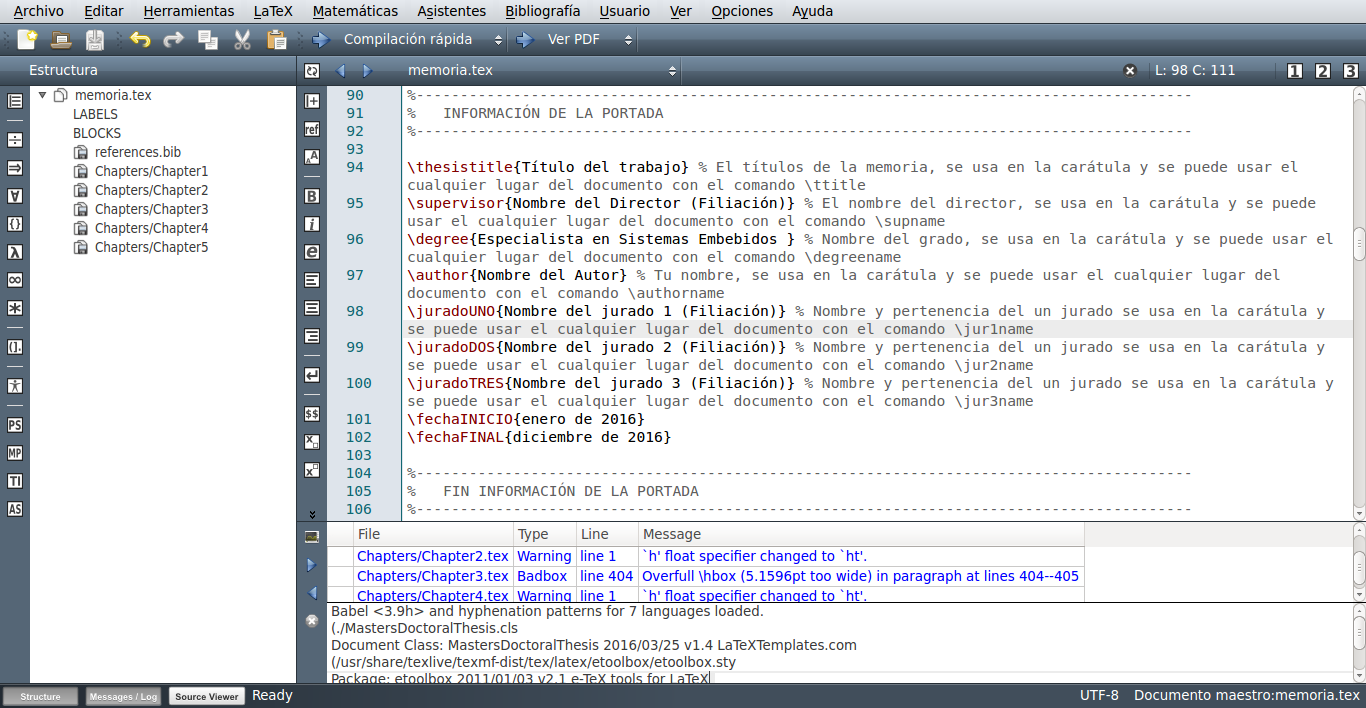
\includegraphics[width=.5\textwidth]{./Figures/texmaker.png}
	\caption{Entorno de trabajo de texMaker.}
	\label{fig:texmaker}
\end{figure}

\vspace{1cm}

Notar que existe una vista llamada Estructura a la izquierda de la interfaz que nos permite abrir desde dentro del programa los archivos individuales de los capítulos.  A la derecha se encuentra una vista con el archivo propiamente dicho para su edición. Hacia la parte inferior se encuentra una vista del log con información de los resultados de la compilación.  En esta última vista pueden aparecen advertencias o \textit{warning}, que normalmente pueden ser ignorados, y los errores que se indican en color rojo y deben resolverse para que se genere el PDF de salida.

Recordar que el archivo que se debe compilar con PDFLaTeX es \file{memoria.tex}, si se tratara de compilar alguno de los capítulos saldría un error.  Para salvar la molestia de tener que cambiar de archivo para compilar cada vez que se realice una modificación en un capítulo, se puede definir el archivo \file{memoria.tex} como ``documento maestro'' yendo al menú opciones -> ``definir documento actual como documento maestro'', lo que permite compilar con PDFLaTeX memoria.tex directamente desde cualquier archivo que se esté modificando . Se muestra esta opción en la figura \ref{fig:docMaestro}.

\begin{figure}[h]
	\centering
	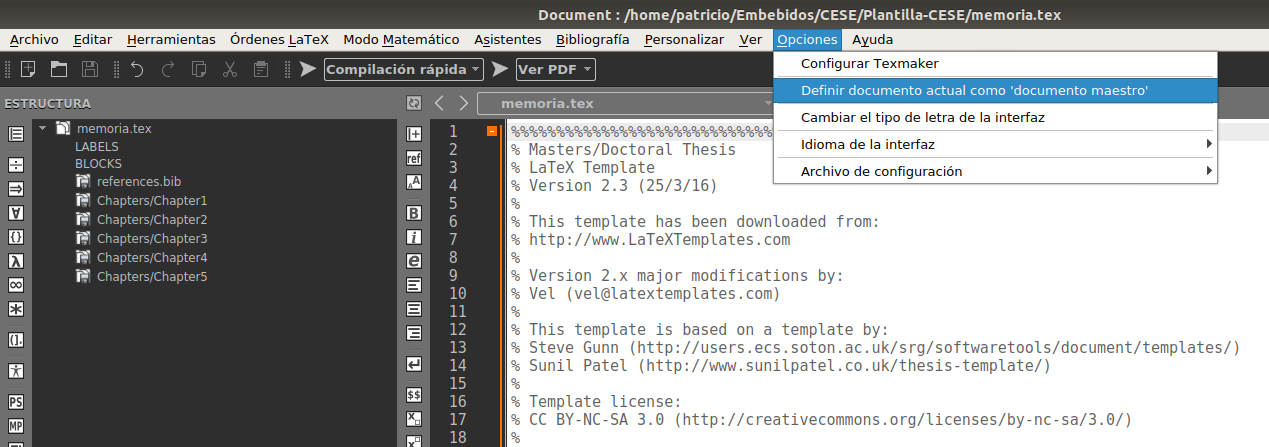
\includegraphics[width=\textwidth]{./Figures/docMaestro.png}
	\caption{Definir memoria.tex como documento maestro.}
	\label{fig:docMaestro}
\end{figure}

En el menú herramientas se encuentran las opciones de compilación.  Para producir un archivo PDF a partir de un archivo .tex se debe ejecutar PDFLaTeX (el shortcut es F6). Para incorporar nueva bibliografía se debe utilizar la opción BibTeX del mismo menú herramientas (el shortcut es F11).

Notar que para actualizar las tablas de contenidos se debe ejecutar PDFLaTeX dos veces.  Esto se debe a que es necesario actualizar algunos archivos auxiliares antes de obtener el resultado final.  En forma similar, para actualizar las referencias se debe ejecutar primero PDFLaTeX, después BibTeX y finalmente PDFLaTeX dos veces por idénticos motivos.

\section{Personalizando la plantilla, el archivo \file{memoria.tex}}
\label{sec:FillingFile}

Para personalizar la plantilla se debe incorporar la información propia en los distintos archivos \file{.tex}. 

Primero abrir \file{memoria.tex} con TexMaker (o el editor de su preferencia). Se debe ubicar dentro del archivo el bloque de código titulado \emph{INFORMACIÓN DE LA PORTADA} donde se deben incorporar los primeros datos personales con los que se construirá automáticamente la portada.


%----------------------------------------------------------------------------------------

\section{El código del archivo \file{memoria.tex} explicado}

El archivo \file{memoria.tex} contiene la estructura del documento y es el archivo de mayor jerarquía de la memoria.  Podría ser equiparable a la función \emph{main()} de un programa en C, o mejor dicho al archivo fuente .c donde se encuentra definida la función main().

La estructura básica de cualquier documento de \LaTeX{} comienza con la definición de clase del documento, es seguida por un preámbulo donde se pueden agregar funcionalidades con el uso de \texttt{paquetes} (equiparables a bibliotecas de C), y finalmente, termina con el cuerpo del documento, donde irá el contenido de la memoria.

\lstset{%
  basicstyle=\small\ttfamily,
  language=[LaTeX]{TeX}
}

\begin{lstlisting}
\documentclass{article}  <- Definicion de clase
\usepackage{listings}	 <- Preambulo

\begin{document}	 <- Comienzo del contenido propio 
	Hello world!
\end{document}
\end{lstlisting}


El archivo \file{memoria.tex} se encuentra densamente comentado para explicar qué páginas, secciones y elementos de formato está creando el código \LaTeX{} en cada línea. El código está dividido en bloques con nombres en mayúsculas para que resulte evidente qué es lo que hace esa porción de código en particular. Inicialmente puede parecer que hay mucho código \LaTeX{}, pero es principalmente código para dar formato a la memoria por lo que no requiere intervención del usuario de la plantilla.  Sí se deben personalizar con su información los bloques indicados como:

\begin{itemize}
	\item Informacion de la memoria
	\item Resumen
	\item Agradecimientos
	\item Dedicatoria
\end{itemize}

El índice de contenidos, las listas de figura de tablas se generan en forma automática y no requieren intervención ni edición manual por parte del usuario de la plantilla. 

En la parte final del documento se encuentran los capítulos y los apéndices.  Por defecto se incluyen los 5 capítulos propuestos que se encuentran en la carpeta /Chapters. Cada capítulo se debe escribir en un archivo .tex separado y se debe poner en la carpeta \emph{Chapters} con el nombre \file{Chapter1}, \file{Chapter2}, etc\ldots El código para incluir capítulos desde archivos externos se muestra a continuación.

\begin{verbatim}
	% Chapter 1

\chapter{Introducción general} % Main chapter title

\label{Chapter1} % For referencing the chapter elsewhere, use \ref{Chapter1} 
\label{IntroGeneral}

%----------------------------------------------------------------------------------------

% Define some commands to keep the formatting separated from the content 
\newcommand{\keyword}[1]{\textbf{#1}}
\newcommand{\tabhead}[1]{\textbf{#1}}
\newcommand{\code}[1]{\texttt{#1}}
\newcommand{\file}[1]{\texttt{\bfseries#1}}
\newcommand{\option}[1]{\texttt{\itshape#1}}
\newcommand{\grados}{$^{\circ}$}

%----------------------------------------------------------------------------------------

%\section{Introducción}

%----------------------------------------------------------------------------------------
\section{Aprendiendo \LaTeX{}}

\LaTeX{} no es \textsc{WYSIWYG} (What You See is What You Get), a diferencia de los procesadores de texto como Microsoft Word o Pages de Apple o incluso LibreOffice en el mundo open-source. En lugar de ello, un documento escrito para \LaTeX{} es en realidad un archivo de texto simple o llano que \emph{no contiene formato} . Nosotros le decimos a \LaTeX{} cómo deseamos que se aplique el formato en el documento final escribiendo comandos simples entre el texto, por ejemplo, si quiero usar texto en itálicas para dar énfasis, escribo \verb|\it{texto}| y pongo el texto que quiero en itálicas entre medio de las llaves. Esto significa que \LaTeX{} es un lenguaje del tipo \enquote{mark-up}, muy parecido a HTML.

\subsection{Una introducción (no tan corta) a \LaTeX{}}

Si sos nuevo en \LaTeX{}, hay un muy buen libro electrónico - disponible gratuitamente en Internet como un archivo PDF - llamado, \enquote{A (not so short) Introduction to \LaTeX{}}. El título del libro es generalmente acortado a simplemente \emph{lshort}. Puede descargar la versión más reciente en inglés (ya que se actualiza de vez en cuando) desde aquí:
\url{http://www.ctan.org/tex-archive/info/lshort/english/lshort.pdf}

Se puede encontrar la versión en español en la lista en esta página: \url{http://www.ctan.org/tex-archive/info/lshort/}

\subsubsection{Una subsubsección}

Acá tiene un ejemplo de una ``subsubsección'' que es el cuarto nivel de ordenamiento del texto, después de capítulo, sección y subsección.  Como se puede ver, las subsubsecciones no van numeradas en el cuerpo del documento ni en el índice.  El formato está definido por la plantilla y no debe ser modificado.

\subsection{Guía matemática rápida para \LaTeX{}}

Si estás escribiendo un documento con mucho contenido matemático, entonces es posible que desees leer el documento de la AMS (American Mathematical Society) llamado, \enquote{A Short Math Guide for \LaTeX{}}. Se puede encontrar en línea en el siguiente link: \url{http://www.ams.org/tex/amslatex.html} en la sección \enquote{Additional Documentation} hacia la parte inferior de la página.


%----------------------------------------------------------------------------------------

\section{Utilizando esta plantilla}

Si estás familiarizado con \LaTeX{}, entonces podés explorar la estructura de directorios de esta plantilla y proceder a personalizarla agregando tu información en el bloque \emph{INFORMACIÓN DE LA PORTADA} en el archivo \file{memoria.tex}.  

Se puede continuar luego modificando el resto de los archivos siguiendo los lineamientos que se describen en la sección \ref{sec:FillingFile} en la página \pageref{sec:FillingFile}.

Debés asegurarte de leer el capítulo \ref{Chapter2} acerca de las convenciones utilizadas para las Memoria de los Trabajos Finales de la \degreename.

Si sos nuevo en \LaTeX{}, se recomienda que continúes leyendo el documento ya que contiene información básica para aprovechar el potencial de esta herramienta.


%----------------------------------------------------------------------------------------

\section{Qué incluye esta plantilla}

\subsection{Carpetas}

Esta plantilla se distribuye como una único archivo .zip que se puede descomprimir en varios archivos y carpetas. Asimismo, se puede consultar el repositorio git para obtener la última versión de los archivos, \url{https://github.com/patriciobos/Plantilla-CESE.git}. Los nombres de las carpetas son, o pretender ser, auto-explicativos.

\keyword{Appendices} -- Esta es la carpeta donde se deben poner los apéndices. Cada apéndice debe ir en su propio archivo \file{.tex}. Se incluye un ejemplo y una plantilla en la carpeta.

\keyword{Chapters} -- Esta es la carpeta donde se deben poner los capítulos de la memoria. Cada capítulo debe ir un su propio archivo \file{.tex} por separado.  Se ofrece por defecto, la siguiente estructura de capítulos y se recomienda su utilización dentro de lo posible:

\begin{itemize}
\item Capítulo 1: Introducción general	
\item Capítulo 2: Introducción específica
\item Capítulo 3: Diseño e implementación
\item Capítulo 4: Ensayos y resultados
\item Capítulo 5: Conclusiones

\end{itemize}

Esta estructura de capítulos es la que se recomienda para las memorias de la especialización.

\keyword{Figures} -- Esta carpeta contiene todas las figuras de la memoria.  Estas son las versiones finales de las imágenes que van a ser incluidas en la memoria.  Pueden ser imágenes en formato \textit{raster}\footnote{\url{https://en.wikipedia.org/wiki/Raster_graphics}} como \file{.png}, \file{.jpg} o en formato vectoriales\footnote{\url{https://en.wikipedia.org/wiki/Vector_graphics}} como \file{.pdf}, \file{.ps}.  Se debe notar que utilizar imágenes vectoriales disminuye notablemente el peso del documento final y acelera el tiempo de compilación por lo que es recomendable su utilización siempre que sea posible.

\subsection{Archivos}

También están incluidos varios archivos, la mayoría de ellos son de texto plano y se puede ver su contenido en un editor de texto. Después de la compilación inicial, se verá que más archivos auxiliares son creados por \ LaTeX{} o BibTeX, pero son de uso interno y no es necesario hacer nada en particular con ellos.  Toda la información necesaria para compilar el documento se encuentra en los archivos \file{.tex}, \file{.bib}, \file{.cls} y en las imágenes de la carpeta Figures.

\keyword{referencias.bib} - este es un archivo importante que contiene toda la información de referencias bibliográficas que se utilizarán para las citas en la memoria en conjunto con BibTeX. Usted puede escribir las entradas bibliográficas en forma manual, aunque existen también programas de gestión de referencias que facilitan la creación y gestión de las referencias y permiten exportarlas en formato BibTeX.  También hay disponibles sitios web como \url{books.google.com} que permiten obtener toda la información necesaria para una cita en formato BibTeX. Ver sección \ref{sec:biblio}

\keyword{MastersDoctoralThesis.cls} -- este es un archivo importante. Es el archivos con la clase que le informa a \LaTeX{} cómo debe dar formato a la memoria. El usuario de la plantilla no debería necesitar modificar nada de este archivo.

\keyword{memoria.pdf} -- esta es su memoria con una tipografía bellamente compuesta (en formato de archivo PDF) creado por \LaTeX{}. Se distribuye con la plantilla y después de compilar por primera vez sin hacer ningún cambio se debería obtener una versión idéntica a este documento.

\keyword{memoria.tex} -- este es un archivo importante. Este es el archivo que tiene que compilar \LaTeX{} para producir la memoria como un archivo PDF. Contiene un marco de trabajo y estructuras que le indican a \LaTeX{} cómo diagramar la memoria.  Está altamente comentado para que se pueda entender qué es lo que realiza cada línea de código y por qué está incluida en ese lugar.  En este archivo se debe completar la información personalizada de las primeras sección según se indica en la sección \ref{sec:FillingFile}.

Archivos que \emph{no} forman parte de la distribución de la plantilla pero que son generados por \LaTeX{} como archivos auxiliares necesarios para la producción de la memoria.pdf son:

\keyword{memoria.aux} -- este es un archivo auxiliar generado por \LaTeX{}, si se borra \LaTeX{} simplemente lo regenera cuando se compila el archivo principal \file{memoria.tex}.

\keyword{memoria.bbl} -- este es un archivo auxiliar generado por BibTeX, si se borra BibTeX simplemente lo regenera cuando se compila el archivo principal \file{memoria.tex}. Mientras que el archivo \file{.bib} contiene todas las referencias que hay, este archivo \file{.bbl} contine sólo las referencias que han sido citadas y se utiliza para la construcción de la bibiografía.

\keyword{memoria.blg} -- este es un archivo auxiliar generado por BibTeX, si se borra BibTeX simplemente lo regenera cuando se compila el archivo principal \file{memoria.tex}.

\keyword{memoria.lof} -- este es un archivo auxiliar generado por \LaTeX{}, si se borra \LaTeX{} simplemente lo regenera cuando se compila el archivo principal \file{memoria.tex}.  Le indica a \LaTeX{} cómo construir la sección \emph{Lista de Figuras}.
 
\keyword{memoria.log} --  este es un archivo auxiliar generado por \LaTeX{}, si se borra \LaTeX{} simplemente lo regenera cuando se compila el archivo principal \file{memoria.tex}. Contiene mensajes de \LaTeX{}. Si se reciben errores o advertencias durante la compilación, se guardan en este archivo \file{.log}.

\keyword{memoria.lot} -- este es un archivo auxiliar generado por \LaTeX{}, si se borra \LaTeX{} simplemente lo regenera cuando se compila el archivo principal \file{memoria.tex}.  Le indica a \LaTeX{} cómo construir la sección \emph{Lista de Tablas}.

\keyword{memoria.out} -- este es un archivo auxiliar generado por \LaTeX{}, si se borra \LaTeX{} simplemente lo regenera cuando se compila el archivo principal \file{memoria.tex}.

De esta larga lista de archivos, sólo aquellos con la extensión \file{.bib}, \file{.cls} y \file{.tex} son importantes.  Los otros archivos auxiliares pueden ser ignorados o borrados ya que \LaTeX{} y BibTeX los regenerarán durante la compilación.

%----------------------------------------------------------------------------------------

\section{Entorno de trabajo}

Ante de comenzar a editar la plantilla debemos tener un editor \LaTeX{} instalado en nuestra computadora.  En forma análoga a lo que sucede en lenguaje C, que se puede crear y editar código con casi cualquier editor, existen ciertos entornos de trabajo que nos pueden simplificar mucho la tarea.  En este sentido, se recomienda, sobre todo para los principiantes en \LaTeX{} la utilización de TexMaker, un programa gratuito y multi-plantaforma que está disponible tanto para windows como para sistemas GNU/linux.

La versión más reciente de TexMaker es la 4.5 y se puede descargar del siguiente link: \url{http://www.xm1math.net/texmaker/download.html}. Se puede consultar el manual de usuario en el siguiente link: \url{http://www.xm1math.net/texmaker/doc.html}.
 

\subsection{Paquetes adicionales}

Si bien durante el proceso de instalación de TexMaker, o cualquier otro editor que se haya elegido, se instalarán en el sistema los paquetes básicos necesarios para trabajar con \LaTeX{}, la plantilla de los trabajos de Especialización y Maestría requieren de paquete adicionales.

Se indican a continuación los comandos que se deben introducir en la consola de Ubuntu (ctrl + alt + t) para instalarlos:

\begin{lstlisting}[language=bash]
  $ sudo apt install texlive-lang-spanish texlive-science 
  $ sudo apt install texlive-bibtex-extra biber
  $ sudo apt install texlive texlive-fonts-recommended
  $ sudo apt install texlive-latex-extra
\end{lstlisting}


\subsection{Configurando TexMaker}



Una vez instalado el programa y los paquetes adicionales se debe abrir el archivo memoria.tex con el editor para ver una pantalla similar a la que se puede apreciar en la figura \ref{fig:texmaker}. 
Una vez instalado el programa y los paquetes adicionales se debe abrir el archivo memoria.tex con el editor para ver una pantalla similar a la que se puede apreciar en la figura \ref{fig:texmaker}. 
Una vez instalado el programa y los paquetes adicionales se debe abrir el archivo memoria.tex con el editor para ver una pantalla similar a la que se puede apreciar en la figura \ref{fig:texmaker}. 
Una vez instalado el programa y los paquetes adicionales se debe abrir el archivo memoria.tex con el editor para ver una pantalla similar a la que se puede apreciar en la figura \ref{fig:texmaker}. 

\vspace{1cm}

\begin{figure}[htbp]
	\centering
	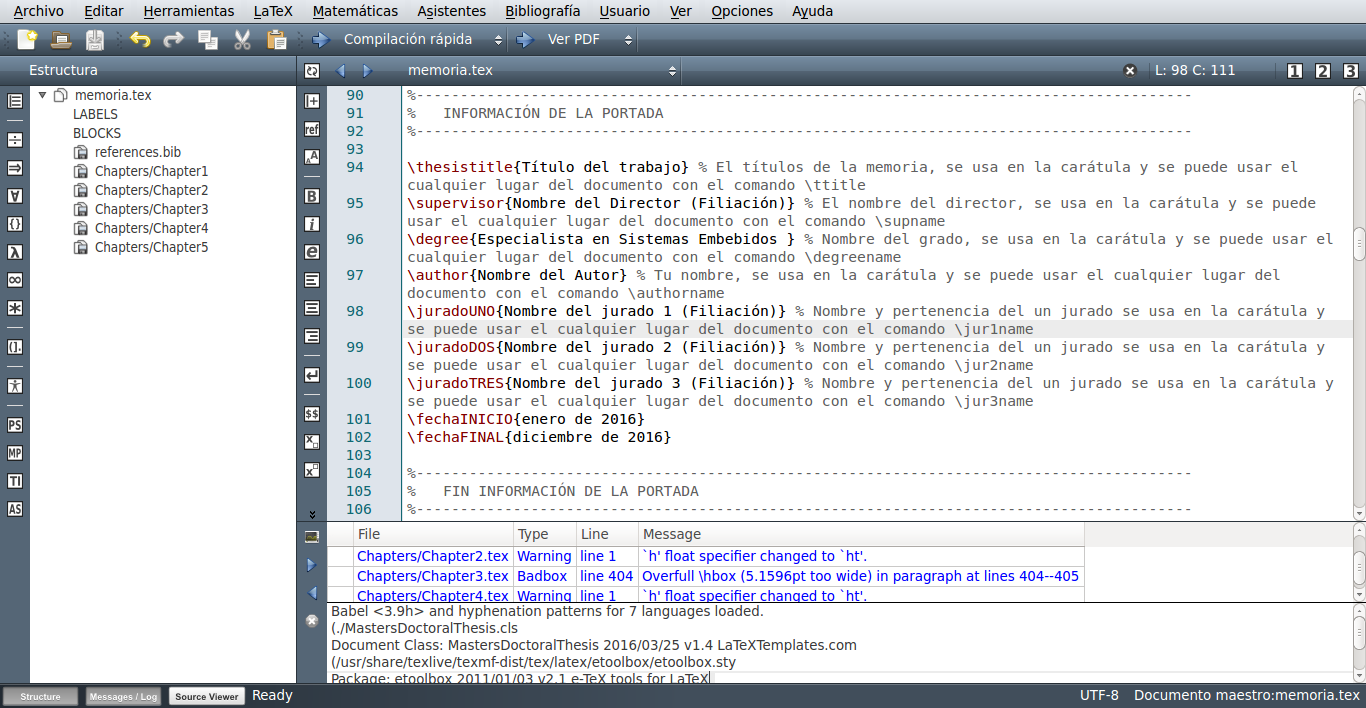
\includegraphics[width=.5\textwidth]{./Figures/texmaker.png}
	\caption{Entorno de trabajo de texMaker.}
	\label{fig:texmaker}
\end{figure}

\vspace{1cm}

Notar que existe una vista llamada Estructura a la izquierda de la interfaz que nos permite abrir desde dentro del programa los archivos individuales de los capítulos.  A la derecha se encuentra una vista con el archivo propiamente dicho para su edición. Hacia la parte inferior se encuentra una vista del log con información de los resultados de la compilación.  En esta última vista pueden aparecen advertencias o \textit{warning}, que normalmente pueden ser ignorados, y los errores que se indican en color rojo y deben resolverse para que se genere el PDF de salida.

Recordar que el archivo que se debe compilar con PDFLaTeX es \file{memoria.tex}, si se tratara de compilar alguno de los capítulos saldría un error.  Para salvar la molestia de tener que cambiar de archivo para compilar cada vez que se realice una modificación en un capítulo, se puede definir el archivo \file{memoria.tex} como ``documento maestro'' yendo al menú opciones -> ``definir documento actual como documento maestro'', lo que permite compilar con PDFLaTeX memoria.tex directamente desde cualquier archivo que se esté modificando . Se muestra esta opción en la figura \ref{fig:docMaestro}.

\begin{figure}[h]
	\centering
	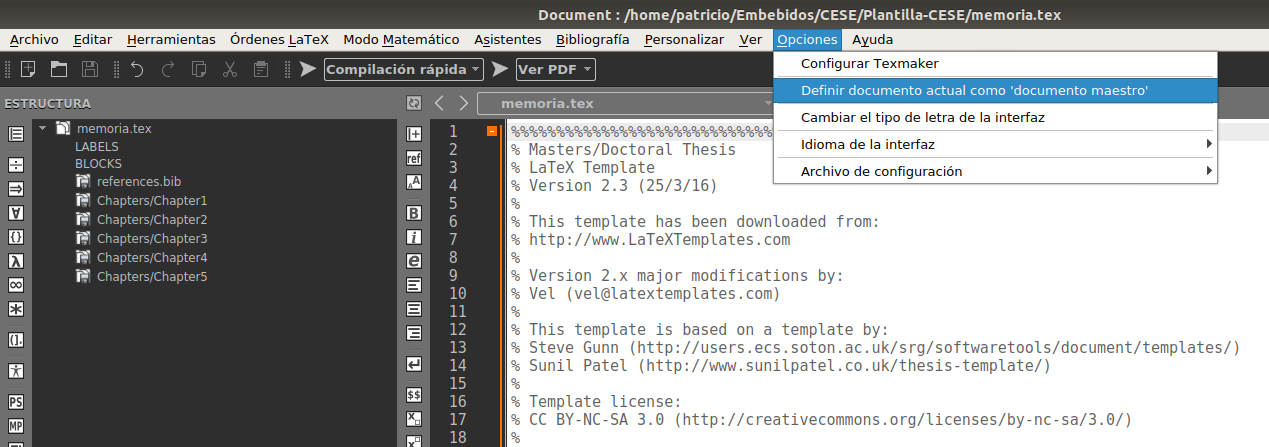
\includegraphics[width=\textwidth]{./Figures/docMaestro.png}
	\caption{Definir memoria.tex como documento maestro.}
	\label{fig:docMaestro}
\end{figure}

En el menú herramientas se encuentran las opciones de compilación.  Para producir un archivo PDF a partir de un archivo .tex se debe ejecutar PDFLaTeX (el shortcut es F6). Para incorporar nueva bibliografía se debe utilizar la opción BibTeX del mismo menú herramientas (el shortcut es F11).

Notar que para actualizar las tablas de contenidos se debe ejecutar PDFLaTeX dos veces.  Esto se debe a que es necesario actualizar algunos archivos auxiliares antes de obtener el resultado final.  En forma similar, para actualizar las referencias se debe ejecutar primero PDFLaTeX, después BibTeX y finalmente PDFLaTeX dos veces por idénticos motivos.

\section{Personalizando la plantilla, el archivo \file{memoria.tex}}
\label{sec:FillingFile}

Para personalizar la plantilla se debe incorporar la información propia en los distintos archivos \file{.tex}. 

Primero abrir \file{memoria.tex} con TexMaker (o el editor de su preferencia). Se debe ubicar dentro del archivo el bloque de código titulado \emph{INFORMACIÓN DE LA PORTADA} donde se deben incorporar los primeros datos personales con los que se construirá automáticamente la portada.


%----------------------------------------------------------------------------------------

\section{El código del archivo \file{memoria.tex} explicado}

El archivo \file{memoria.tex} contiene la estructura del documento y es el archivo de mayor jerarquía de la memoria.  Podría ser equiparable a la función \emph{main()} de un programa en C, o mejor dicho al archivo fuente .c donde se encuentra definida la función main().

La estructura básica de cualquier documento de \LaTeX{} comienza con la definición de clase del documento, es seguida por un preámbulo donde se pueden agregar funcionalidades con el uso de \texttt{paquetes} (equiparables a bibliotecas de C), y finalmente, termina con el cuerpo del documento, donde irá el contenido de la memoria.

\lstset{%
  basicstyle=\small\ttfamily,
  language=[LaTeX]{TeX}
}

\begin{lstlisting}
\documentclass{article}  <- Definicion de clase
\usepackage{listings}	 <- Preambulo

\begin{document}	 <- Comienzo del contenido propio 
	Hello world!
\end{document}
\end{lstlisting}


El archivo \file{memoria.tex} se encuentra densamente comentado para explicar qué páginas, secciones y elementos de formato está creando el código \LaTeX{} en cada línea. El código está dividido en bloques con nombres en mayúsculas para que resulte evidente qué es lo que hace esa porción de código en particular. Inicialmente puede parecer que hay mucho código \LaTeX{}, pero es principalmente código para dar formato a la memoria por lo que no requiere intervención del usuario de la plantilla.  Sí se deben personalizar con su información los bloques indicados como:

\begin{itemize}
	\item Informacion de la memoria
	\item Resumen
	\item Agradecimientos
	\item Dedicatoria
\end{itemize}

El índice de contenidos, las listas de figura de tablas se generan en forma automática y no requieren intervención ni edición manual por parte del usuario de la plantilla. 

En la parte final del documento se encuentran los capítulos y los apéndices.  Por defecto se incluyen los 5 capítulos propuestos que se encuentran en la carpeta /Chapters. Cada capítulo se debe escribir en un archivo .tex separado y se debe poner en la carpeta \emph{Chapters} con el nombre \file{Chapter1}, \file{Chapter2}, etc\ldots El código para incluir capítulos desde archivos externos se muestra a continuación.

\begin{verbatim}
	% Chapter 1

\chapter{Introducción general} % Main chapter title

\label{Chapter1} % For referencing the chapter elsewhere, use \ref{Chapter1} 
\label{IntroGeneral}

%----------------------------------------------------------------------------------------

% Define some commands to keep the formatting separated from the content 
\newcommand{\keyword}[1]{\textbf{#1}}
\newcommand{\tabhead}[1]{\textbf{#1}}
\newcommand{\code}[1]{\texttt{#1}}
\newcommand{\file}[1]{\texttt{\bfseries#1}}
\newcommand{\option}[1]{\texttt{\itshape#1}}
\newcommand{\grados}{$^{\circ}$}

%----------------------------------------------------------------------------------------

%\section{Introducción}

%----------------------------------------------------------------------------------------
\section{Aprendiendo \LaTeX{}}

\LaTeX{} no es \textsc{WYSIWYG} (What You See is What You Get), a diferencia de los procesadores de texto como Microsoft Word o Pages de Apple o incluso LibreOffice en el mundo open-source. En lugar de ello, un documento escrito para \LaTeX{} es en realidad un archivo de texto simple o llano que \emph{no contiene formato} . Nosotros le decimos a \LaTeX{} cómo deseamos que se aplique el formato en el documento final escribiendo comandos simples entre el texto, por ejemplo, si quiero usar texto en itálicas para dar énfasis, escribo \verb|\it{texto}| y pongo el texto que quiero en itálicas entre medio de las llaves. Esto significa que \LaTeX{} es un lenguaje del tipo \enquote{mark-up}, muy parecido a HTML.

\subsection{Una introducción (no tan corta) a \LaTeX{}}

Si sos nuevo en \LaTeX{}, hay un muy buen libro electrónico - disponible gratuitamente en Internet como un archivo PDF - llamado, \enquote{A (not so short) Introduction to \LaTeX{}}. El título del libro es generalmente acortado a simplemente \emph{lshort}. Puede descargar la versión más reciente en inglés (ya que se actualiza de vez en cuando) desde aquí:
\url{http://www.ctan.org/tex-archive/info/lshort/english/lshort.pdf}

Se puede encontrar la versión en español en la lista en esta página: \url{http://www.ctan.org/tex-archive/info/lshort/}

\subsubsection{Una subsubsección}

Acá tiene un ejemplo de una ``subsubsección'' que es el cuarto nivel de ordenamiento del texto, después de capítulo, sección y subsección.  Como se puede ver, las subsubsecciones no van numeradas en el cuerpo del documento ni en el índice.  El formato está definido por la plantilla y no debe ser modificado.

\subsection{Guía matemática rápida para \LaTeX{}}

Si estás escribiendo un documento con mucho contenido matemático, entonces es posible que desees leer el documento de la AMS (American Mathematical Society) llamado, \enquote{A Short Math Guide for \LaTeX{}}. Se puede encontrar en línea en el siguiente link: \url{http://www.ams.org/tex/amslatex.html} en la sección \enquote{Additional Documentation} hacia la parte inferior de la página.


%----------------------------------------------------------------------------------------

\section{Utilizando esta plantilla}

Si estás familiarizado con \LaTeX{}, entonces podés explorar la estructura de directorios de esta plantilla y proceder a personalizarla agregando tu información en el bloque \emph{INFORMACIÓN DE LA PORTADA} en el archivo \file{memoria.tex}.  

Se puede continuar luego modificando el resto de los archivos siguiendo los lineamientos que se describen en la sección \ref{sec:FillingFile} en la página \pageref{sec:FillingFile}.

Debés asegurarte de leer el capítulo \ref{Chapter2} acerca de las convenciones utilizadas para las Memoria de los Trabajos Finales de la \degreename.

Si sos nuevo en \LaTeX{}, se recomienda que continúes leyendo el documento ya que contiene información básica para aprovechar el potencial de esta herramienta.


%----------------------------------------------------------------------------------------

\section{Qué incluye esta plantilla}

\subsection{Carpetas}

Esta plantilla se distribuye como una único archivo .zip que se puede descomprimir en varios archivos y carpetas. Asimismo, se puede consultar el repositorio git para obtener la última versión de los archivos, \url{https://github.com/patriciobos/Plantilla-CESE.git}. Los nombres de las carpetas son, o pretender ser, auto-explicativos.

\keyword{Appendices} -- Esta es la carpeta donde se deben poner los apéndices. Cada apéndice debe ir en su propio archivo \file{.tex}. Se incluye un ejemplo y una plantilla en la carpeta.

\keyword{Chapters} -- Esta es la carpeta donde se deben poner los capítulos de la memoria. Cada capítulo debe ir un su propio archivo \file{.tex} por separado.  Se ofrece por defecto, la siguiente estructura de capítulos y se recomienda su utilización dentro de lo posible:

\begin{itemize}
\item Capítulo 1: Introducción general	
\item Capítulo 2: Introducción específica
\item Capítulo 3: Diseño e implementación
\item Capítulo 4: Ensayos y resultados
\item Capítulo 5: Conclusiones

\end{itemize}

Esta estructura de capítulos es la que se recomienda para las memorias de la especialización.

\keyword{Figures} -- Esta carpeta contiene todas las figuras de la memoria.  Estas son las versiones finales de las imágenes que van a ser incluidas en la memoria.  Pueden ser imágenes en formato \textit{raster}\footnote{\url{https://en.wikipedia.org/wiki/Raster_graphics}} como \file{.png}, \file{.jpg} o en formato vectoriales\footnote{\url{https://en.wikipedia.org/wiki/Vector_graphics}} como \file{.pdf}, \file{.ps}.  Se debe notar que utilizar imágenes vectoriales disminuye notablemente el peso del documento final y acelera el tiempo de compilación por lo que es recomendable su utilización siempre que sea posible.

\subsection{Archivos}

También están incluidos varios archivos, la mayoría de ellos son de texto plano y se puede ver su contenido en un editor de texto. Después de la compilación inicial, se verá que más archivos auxiliares son creados por \ LaTeX{} o BibTeX, pero son de uso interno y no es necesario hacer nada en particular con ellos.  Toda la información necesaria para compilar el documento se encuentra en los archivos \file{.tex}, \file{.bib}, \file{.cls} y en las imágenes de la carpeta Figures.

\keyword{referencias.bib} - este es un archivo importante que contiene toda la información de referencias bibliográficas que se utilizarán para las citas en la memoria en conjunto con BibTeX. Usted puede escribir las entradas bibliográficas en forma manual, aunque existen también programas de gestión de referencias que facilitan la creación y gestión de las referencias y permiten exportarlas en formato BibTeX.  También hay disponibles sitios web como \url{books.google.com} que permiten obtener toda la información necesaria para una cita en formato BibTeX. Ver sección \ref{sec:biblio}

\keyword{MastersDoctoralThesis.cls} -- este es un archivo importante. Es el archivos con la clase que le informa a \LaTeX{} cómo debe dar formato a la memoria. El usuario de la plantilla no debería necesitar modificar nada de este archivo.

\keyword{memoria.pdf} -- esta es su memoria con una tipografía bellamente compuesta (en formato de archivo PDF) creado por \LaTeX{}. Se distribuye con la plantilla y después de compilar por primera vez sin hacer ningún cambio se debería obtener una versión idéntica a este documento.

\keyword{memoria.tex} -- este es un archivo importante. Este es el archivo que tiene que compilar \LaTeX{} para producir la memoria como un archivo PDF. Contiene un marco de trabajo y estructuras que le indican a \LaTeX{} cómo diagramar la memoria.  Está altamente comentado para que se pueda entender qué es lo que realiza cada línea de código y por qué está incluida en ese lugar.  En este archivo se debe completar la información personalizada de las primeras sección según se indica en la sección \ref{sec:FillingFile}.

Archivos que \emph{no} forman parte de la distribución de la plantilla pero que son generados por \LaTeX{} como archivos auxiliares necesarios para la producción de la memoria.pdf son:

\keyword{memoria.aux} -- este es un archivo auxiliar generado por \LaTeX{}, si se borra \LaTeX{} simplemente lo regenera cuando se compila el archivo principal \file{memoria.tex}.

\keyword{memoria.bbl} -- este es un archivo auxiliar generado por BibTeX, si se borra BibTeX simplemente lo regenera cuando se compila el archivo principal \file{memoria.tex}. Mientras que el archivo \file{.bib} contiene todas las referencias que hay, este archivo \file{.bbl} contine sólo las referencias que han sido citadas y se utiliza para la construcción de la bibiografía.

\keyword{memoria.blg} -- este es un archivo auxiliar generado por BibTeX, si se borra BibTeX simplemente lo regenera cuando se compila el archivo principal \file{memoria.tex}.

\keyword{memoria.lof} -- este es un archivo auxiliar generado por \LaTeX{}, si se borra \LaTeX{} simplemente lo regenera cuando se compila el archivo principal \file{memoria.tex}.  Le indica a \LaTeX{} cómo construir la sección \emph{Lista de Figuras}.
 
\keyword{memoria.log} --  este es un archivo auxiliar generado por \LaTeX{}, si se borra \LaTeX{} simplemente lo regenera cuando se compila el archivo principal \file{memoria.tex}. Contiene mensajes de \LaTeX{}. Si se reciben errores o advertencias durante la compilación, se guardan en este archivo \file{.log}.

\keyword{memoria.lot} -- este es un archivo auxiliar generado por \LaTeX{}, si se borra \LaTeX{} simplemente lo regenera cuando se compila el archivo principal \file{memoria.tex}.  Le indica a \LaTeX{} cómo construir la sección \emph{Lista de Tablas}.

\keyword{memoria.out} -- este es un archivo auxiliar generado por \LaTeX{}, si se borra \LaTeX{} simplemente lo regenera cuando se compila el archivo principal \file{memoria.tex}.

De esta larga lista de archivos, sólo aquellos con la extensión \file{.bib}, \file{.cls} y \file{.tex} son importantes.  Los otros archivos auxiliares pueden ser ignorados o borrados ya que \LaTeX{} y BibTeX los regenerarán durante la compilación.

%----------------------------------------------------------------------------------------

\section{Entorno de trabajo}

Ante de comenzar a editar la plantilla debemos tener un editor \LaTeX{} instalado en nuestra computadora.  En forma análoga a lo que sucede en lenguaje C, que se puede crear y editar código con casi cualquier editor, existen ciertos entornos de trabajo que nos pueden simplificar mucho la tarea.  En este sentido, se recomienda, sobre todo para los principiantes en \LaTeX{} la utilización de TexMaker, un programa gratuito y multi-plantaforma que está disponible tanto para windows como para sistemas GNU/linux.

La versión más reciente de TexMaker es la 4.5 y se puede descargar del siguiente link: \url{http://www.xm1math.net/texmaker/download.html}. Se puede consultar el manual de usuario en el siguiente link: \url{http://www.xm1math.net/texmaker/doc.html}.
 

\subsection{Paquetes adicionales}

Si bien durante el proceso de instalación de TexMaker, o cualquier otro editor que se haya elegido, se instalarán en el sistema los paquetes básicos necesarios para trabajar con \LaTeX{}, la plantilla de los trabajos de Especialización y Maestría requieren de paquete adicionales.

Se indican a continuación los comandos que se deben introducir en la consola de Ubuntu (ctrl + alt + t) para instalarlos:

\begin{lstlisting}[language=bash]
  $ sudo apt install texlive-lang-spanish texlive-science 
  $ sudo apt install texlive-bibtex-extra biber
  $ sudo apt install texlive texlive-fonts-recommended
  $ sudo apt install texlive-latex-extra
\end{lstlisting}


\subsection{Configurando TexMaker}



Una vez instalado el programa y los paquetes adicionales se debe abrir el archivo memoria.tex con el editor para ver una pantalla similar a la que se puede apreciar en la figura \ref{fig:texmaker}. 
Una vez instalado el programa y los paquetes adicionales se debe abrir el archivo memoria.tex con el editor para ver una pantalla similar a la que se puede apreciar en la figura \ref{fig:texmaker}. 
Una vez instalado el programa y los paquetes adicionales se debe abrir el archivo memoria.tex con el editor para ver una pantalla similar a la que se puede apreciar en la figura \ref{fig:texmaker}. 
Una vez instalado el programa y los paquetes adicionales se debe abrir el archivo memoria.tex con el editor para ver una pantalla similar a la que se puede apreciar en la figura \ref{fig:texmaker}. 

\vspace{1cm}

\begin{figure}[htbp]
	\centering
	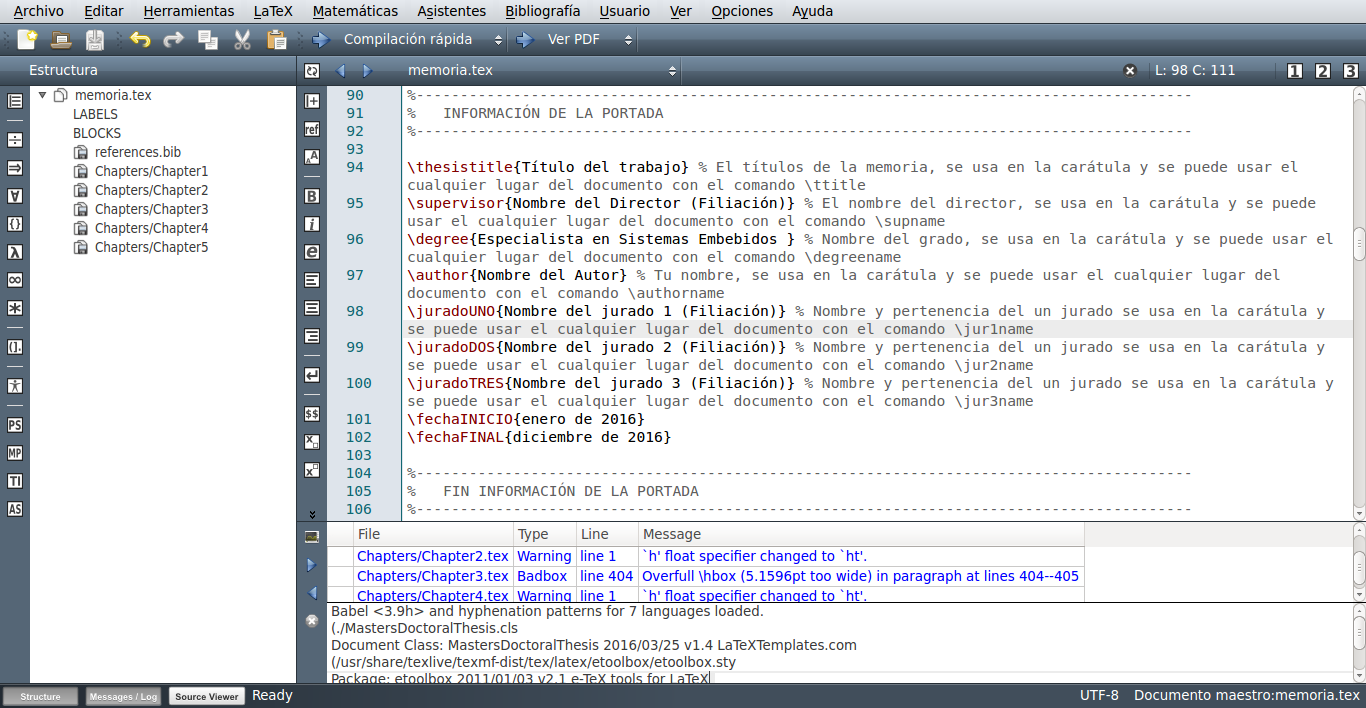
\includegraphics[width=.5\textwidth]{./Figures/texmaker.png}
	\caption{Entorno de trabajo de texMaker.}
	\label{fig:texmaker}
\end{figure}

\vspace{1cm}

Notar que existe una vista llamada Estructura a la izquierda de la interfaz que nos permite abrir desde dentro del programa los archivos individuales de los capítulos.  A la derecha se encuentra una vista con el archivo propiamente dicho para su edición. Hacia la parte inferior se encuentra una vista del log con información de los resultados de la compilación.  En esta última vista pueden aparecen advertencias o \textit{warning}, que normalmente pueden ser ignorados, y los errores que se indican en color rojo y deben resolverse para que se genere el PDF de salida.

Recordar que el archivo que se debe compilar con PDFLaTeX es \file{memoria.tex}, si se tratara de compilar alguno de los capítulos saldría un error.  Para salvar la molestia de tener que cambiar de archivo para compilar cada vez que se realice una modificación en un capítulo, se puede definir el archivo \file{memoria.tex} como ``documento maestro'' yendo al menú opciones -> ``definir documento actual como documento maestro'', lo que permite compilar con PDFLaTeX memoria.tex directamente desde cualquier archivo que se esté modificando . Se muestra esta opción en la figura \ref{fig:docMaestro}.

\begin{figure}[h]
	\centering
	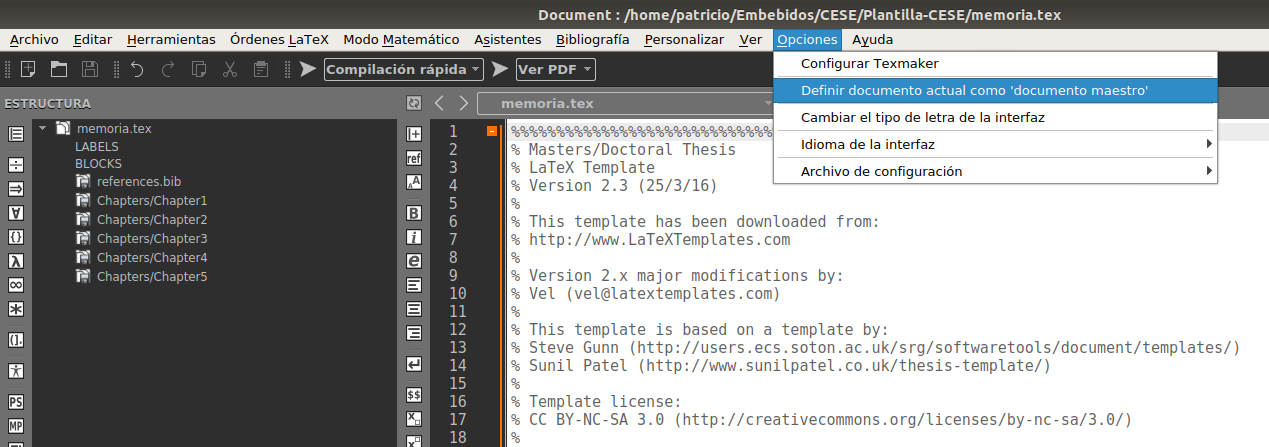
\includegraphics[width=\textwidth]{./Figures/docMaestro.png}
	\caption{Definir memoria.tex como documento maestro.}
	\label{fig:docMaestro}
\end{figure}

En el menú herramientas se encuentran las opciones de compilación.  Para producir un archivo PDF a partir de un archivo .tex se debe ejecutar PDFLaTeX (el shortcut es F6). Para incorporar nueva bibliografía se debe utilizar la opción BibTeX del mismo menú herramientas (el shortcut es F11).

Notar que para actualizar las tablas de contenidos se debe ejecutar PDFLaTeX dos veces.  Esto se debe a que es necesario actualizar algunos archivos auxiliares antes de obtener el resultado final.  En forma similar, para actualizar las referencias se debe ejecutar primero PDFLaTeX, después BibTeX y finalmente PDFLaTeX dos veces por idénticos motivos.

\section{Personalizando la plantilla, el archivo \file{memoria.tex}}
\label{sec:FillingFile}

Para personalizar la plantilla se debe incorporar la información propia en los distintos archivos \file{.tex}. 

Primero abrir \file{memoria.tex} con TexMaker (o el editor de su preferencia). Se debe ubicar dentro del archivo el bloque de código titulado \emph{INFORMACIÓN DE LA PORTADA} donde se deben incorporar los primeros datos personales con los que se construirá automáticamente la portada.


%----------------------------------------------------------------------------------------

\section{El código del archivo \file{memoria.tex} explicado}

El archivo \file{memoria.tex} contiene la estructura del documento y es el archivo de mayor jerarquía de la memoria.  Podría ser equiparable a la función \emph{main()} de un programa en C, o mejor dicho al archivo fuente .c donde se encuentra definida la función main().

La estructura básica de cualquier documento de \LaTeX{} comienza con la definición de clase del documento, es seguida por un preámbulo donde se pueden agregar funcionalidades con el uso de \texttt{paquetes} (equiparables a bibliotecas de C), y finalmente, termina con el cuerpo del documento, donde irá el contenido de la memoria.

\lstset{%
  basicstyle=\small\ttfamily,
  language=[LaTeX]{TeX}
}

\begin{lstlisting}
\documentclass{article}  <- Definicion de clase
\usepackage{listings}	 <- Preambulo

\begin{document}	 <- Comienzo del contenido propio 
	Hello world!
\end{document}
\end{lstlisting}


El archivo \file{memoria.tex} se encuentra densamente comentado para explicar qué páginas, secciones y elementos de formato está creando el código \LaTeX{} en cada línea. El código está dividido en bloques con nombres en mayúsculas para que resulte evidente qué es lo que hace esa porción de código en particular. Inicialmente puede parecer que hay mucho código \LaTeX{}, pero es principalmente código para dar formato a la memoria por lo que no requiere intervención del usuario de la plantilla.  Sí se deben personalizar con su información los bloques indicados como:

\begin{itemize}
	\item Informacion de la memoria
	\item Resumen
	\item Agradecimientos
	\item Dedicatoria
\end{itemize}

El índice de contenidos, las listas de figura de tablas se generan en forma automática y no requieren intervención ni edición manual por parte del usuario de la plantilla. 

En la parte final del documento se encuentran los capítulos y los apéndices.  Por defecto se incluyen los 5 capítulos propuestos que se encuentran en la carpeta /Chapters. Cada capítulo se debe escribir en un archivo .tex separado y se debe poner en la carpeta \emph{Chapters} con el nombre \file{Chapter1}, \file{Chapter2}, etc\ldots El código para incluir capítulos desde archivos externos se muestra a continuación.

\begin{verbatim}
	\include{Chapters/Chapter1}
	\include{Chapters/Chapter2} 
	\include{Chapters/Chapter3}
	\include{Chapters/Chapter4} 
	\include{Chapters/Chapter5} 
\end{verbatim}

Los apéndices también deben escribirse en archivos .tex separados, que se deben ubicar dentro de la carpeta \emph{Appendices}. Los apéndices vienen comentados por defecto con el caracter \code{\%} y para incluirlos simplemente se debe eliminar dicho caracter.

Finalmente, se encuentra el código para incluir la bibliografía en el documento final.  Este código tampoco debe modificarse. La metodología para trabajar las referencias bibliográficas se desarrolla en la sección \ref{sec:biblio}.
%----------------------------------------------------------------------------------------

\section{Bibliografía}
\label{sec:biblio}

Las opciones de formato de la bibliografía se controlan a través del paquete de latex \option{biblatex} que se incluye en la memoria en el archivo memoria.tex.  Estas opciones determinan cómo se generan las citas bibliográficas en el cuerpo del documento y cómo se genera la bibliografía al final de la memoria.

En el preámbulo se puede encontrar el código que incluye el paquete biblatex, que no requiere ninguna modificación del usuario de la plantilla, y que contiene las siguientes opciones:

\begin{lstlisting}
\usepackage[backend=bibtex,
	natbib=true, 
	style=numeric, 
	sorting=none]
{biblatex}
\end{lstlisting}

En el archivo \file{reference.bib} se encuentran las referencias bibliográficas que se pueden citar en el documento.  Para incorporar una nueva cita al documento lo primero es agregarla en este archivo con todos los campos necesario.  Todas las entradas bibliográficas comienzan con $@$ y una palabra que define el formato de la entrada.  Para cada formato existen campos obligatorios que deben completarse. No importa el orden en que las entradas estén definidas en el archivo .bib.  Tampoco es importante el orden en que estén definidos los campos de una entrada bibliográfica. A continuación se muestran algunos ejemplos:

\begin{lstlisting}
@ARTICLE{ARTICLE:1,
    AUTHOR="John Doe",
    TITLE="Title",
    JOURNAL="Journal",
    YEAR="2017",
}
\end{lstlisting}


\begin{lstlisting}
@BOOK{BOOK:1,
    AUTHOR="John Doe",
    TITLE="The Book without Title",
    PUBLISHER="Dummy Publisher",
    YEAR="2100",
}
\end{lstlisting}


\begin{lstlisting}
@INBOOK{BOOK:2,
    AUTHOR="John Doe",
    TITLE="The Book without Title",
    PUBLISHER="Dummy Publisher",
    YEAR="2100",
    PAGES="100-200",
}
\end{lstlisting}


\begin{lstlisting}
@MISC{WEBSITE:1,
    HOWPUBLISHED = "\url{http://example.com}",
    AUTHOR = "Intel",
    TITLE = "Example Website",
    MONTH = "12",
    YEAR = "1988",
    URLDATE = {2012-11-26}
}
\end{lstlisting}

Se debe notar que los nombres \emph{ARTICLE:1}, \emph{BOOK:1}, \emph{BOOK:2} y \emph{WEBSITE:1} son nombres de fantasía que le sirve al autor del documento para identificar la entrada. En este sentido, se podrían reemplazar por cualquier otro nombre.  Tampoco es necesario poner : seguido de un número, en los ejemplos sólo se incluye como un posible estilo para identificar las entradas.

La entradas se citan en el documento con el comando: 

\begin{verbatim}
\citep{nombre_de_la_entrada}
\end{verbatim}

Y cuando se usan, se muestran así: \citep{ARTICLE:1}, \citep{BOOK:1}, \citep{BOOK:2}, \citep{WEBSITE:1}.  Notar cómo se conforma la sección Bibliografía al final del documento. 

	\chapter{Introducción específica}

\label{Chapter2}

En este capítulo se detallan las tecnologías que forman parte del trabajo.
Son productos de terceros que se integran en las herramientas entregadas al cliente.

\section{Arquitectura del dispositivo bajo prueba}
\label{sec:dut}

El trabajo fue realizado para un tipo de microcontrolador específico.
Su diseño forma parte de la familia \emph{Cortex M7} de la empresa \emph{ARM}.
En la figura \ref{fig:cortexm} se puede observar un diagrama en bloques de la arquitectura.

El dispositivo bajo prueba es el microcontrolador \emph{SAM V71} diseñado por la empresa \emph{Atmel} y comercializado por \emph{Microchip}.
El integrado fue pensado para aplicaciones automotrices según el estándar \emph{ISO-TS-16949}.
Además, el circuito puede operar con un reloj de 300 MHz y almacenar un programa de 2048 kB.
Las estructuras de datos del programa pueden aprovechar la memoria cache dual de 16 kB \citep{ARTICLE:dutdatasheet}.
Las principales características del dispositivo bajo prueba son:

\begin{itemize}
    \item Núcleo:
        \begin{itemize}
            \item Unidad de punto flotante de precisión simple y doble.
            \item Unidad de protección de memoria con 16 zonas.
            \item Instrucciones para el procesamiento digital de señales.
        \end{itemize}
    \item Memorias:
        \begin{itemize}
            \item \emph{ROM} de 16 kB con rutinas de inicialización. Esto permite iniciar el sistema desde los periféricos \emph{UART0} y \emph{USB}.
            \item Controlador de memoria estática para el uso de memorias externas.
        \end{itemize}
    \item Sistema:
        \begin{itemize}
            \item Reloj de tiempo real con gestión de calendario gregoriano.
            \item Reinicio por alimentación, detección de caída de tensión y doble \emph{Watchdog}.
            \item Puerto dual de 24 canales para la gestión de acceso a memoria.
            \item Compensación por variaciones de reloj.
        \end{itemize}
\end{itemize}

\newpage

Este integrado fue sometido a una prueba por radiación donde se evaluaron SEE y la calificación de dosis total de ionización (TID).
El microcontrolador mantuvo su funcionamiento en todo el rango de temperatura de calificación militar.
Además, el dispositivo es inmune a \emph{Single Event Latch-up} con una tolerancia de 60,0 $MeV.cm^2/mg$.
Esta sensibilidad fue probada con una cámara de iones pesados.
En cuanto a la calificación de dosis total de ionización, el lote fue sometido a un ensayo de 30 krad(Si) y la prueba fue superada.
Finalmente, los ensayos suministrados por el fabricante permiten concluir que no es necesario realizar inyecciones de errores en la memoria \emph{flash} \citep{ARTICLE:dutrad}.

Al fabricante del dispositivo bajo prueba se le impone respetar el mapa de memoria y registros del núcleo.
Esto permitió construir un inyector de \emph{soft-errors} genérico.
Finalmente, la herramienta entregada funciona para cualquier integrado de la familia \emph{Cortex M}.

\begin{figure}[htbp]
	\centering
	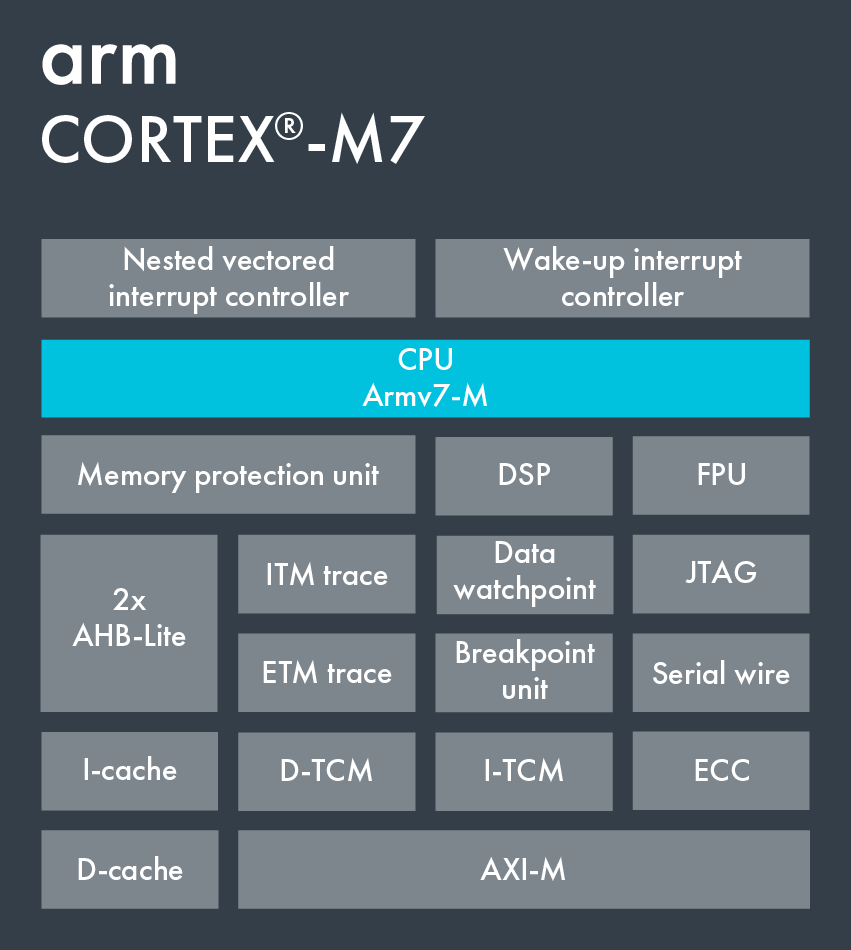
\includegraphics[width=.7\textwidth]{./Figures/Cortex-M7.png}
    \caption{Diagrama de la arquitectura \emph{Cortex M7}\protect\footnotemark.}
	\label{fig:cortexm}
\end{figure}

\footnotetext{Imagen tomada de la página oficial de \emph{ARM Developers}. \citep{WEBSITE:cortexm}}

La arquitectura tiene un módulo que permite programar y depurar el integrado.
Este módulo se denomina \emph{CoreSight} y es propio de los dispositivos \emph{ARM}.
En la figura \ref{fig:coresight} se muestra un diagrama en bloques del módulo.
Sus partes principales son:

\begin{itemize}
    \item \emph{Cross Triggering}: permite conectar y encaminar las señales que utilizan las sondas de depuración.
        En la figura \ref{fig:coresight} está representada en los bloques \emph{CTI}.
        Además, se unen a través del \emph{Cross Trigger Matrix (CTM)}.
    \item \emph{Debug Access Port (DAP)}: es el puerto físico para conectar la sonda de depuración. Es una implementación de la interfaz de depuración \emph{ARM}.
    \item \emph{Embedded Trace Macrocells}: permite extraer información y controlar el núcleo del dispositivo.
    \item \emph{Instrumentation Trace Units}: permite que una sonda de depuración se conecte con las \emph{Embedded Trace Macrocells}.
    \item \emph{ROM Tables}: sirven para que la sonda de depuración identifique al integrado.
    \item \emph{Self Hosted Debug}: son instrucciones específicas de depuración controladas por un procesador secundario.
    \item \emph{Trace Interconnect}: provee puentes para compartir señales de reloj, alimentación y otras señales comunes.
\end{itemize}

\begin{figure}[htbp]
	\centering
	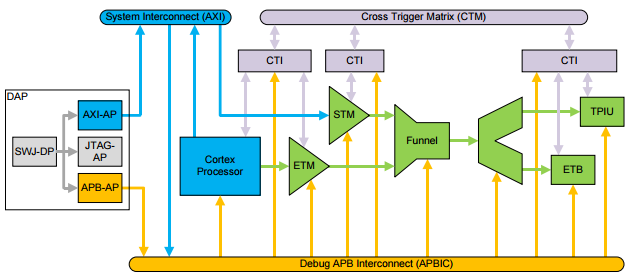
\includegraphics[width=\textwidth]{./Figures/coresight.png}
    \caption{Diagrama del módulo \emph{CoreSight}\protect\footnotemark.}
	\label{fig:coresight}
\end{figure}
\footnotetext{Imagen tomada del artículo \emph{How to debug: CoreSight basis} \citep{WEBSITE:coresight}.}

\section{Servidores y sondas de depuración}
\label{sec:depuracion}

Una sesión de depuración sirve para observar y modificar el estado de ejecución de un programa.
Esto se logra al leer y modificar los valores en registros del procesador y periféricos.
Además, se necesita de un sistema de disparos por eventos y supervisión de recursos.
Finalmente, la sesión debe detener la ejecución del núcleo de ser necesario.
En la figura \ref{fig:debug} se puede observar un esquema simplificado de una sesión de depuración.

\begin{figure}[htbp]
	\centering
	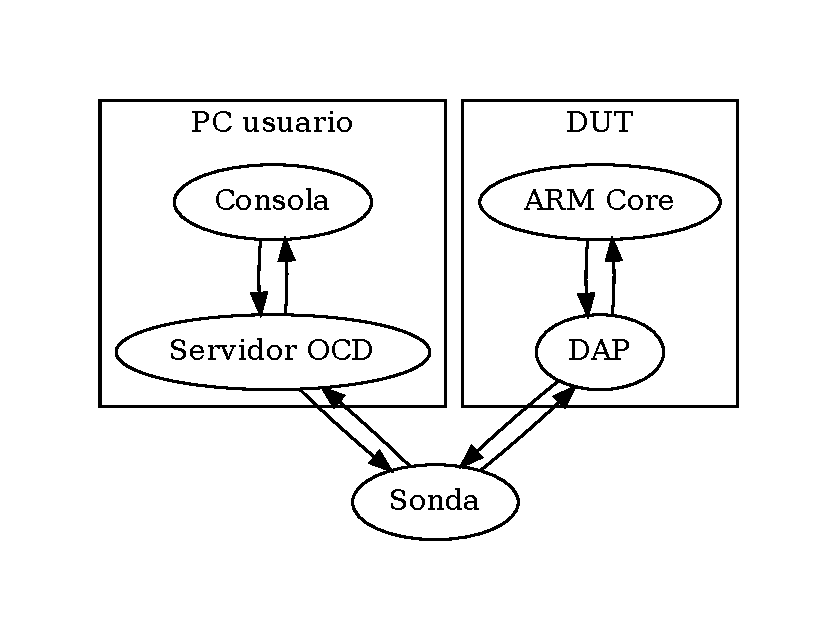
\includegraphics[width=.8\textwidth]{./Figures/debug.pdf}
    \caption{Conexión de una sesión de depuración.}
	\label{fig:debug}
\end{figure}

Un servidor \emph{On-chip debugger (OCD)} tiene la misión de abstraer la conexión de la sonda de depuración.
Además, facilita el manejo del ciclo de vida de la sesión y permite usar un \emph{software} como \emph{GNU Project debugger (GDB)}.
Finalmente, es la base de una pila de tecnologías que permite el uso de herramientas como \emph{GNU Emacs (Emacs)} \citep{BOOK:gdb}.
En la tabla \ref{tab:servidores} se puede observar un resumen de los servidores evaluados en el trabajo.

\begin{table}[h]
	\centering
	\caption[Servidores de depuración]{Comparativa entre servidores de depuración.}
	\begin{tabular}{l c c c}    
		\toprule
        \textbf{Servidor} & \textbf{API} & \textbf{Acceso}   & \textbf{Licencia}\\
		\midrule
        OpenOCD           & tcl                         & Registros y SDRAM & MIT\\        	
        PyOCD             & Python 3                    & Registros y SDRAM & Apache-2.0\\
		\bottomrule
		\hline
	\end{tabular}
	\label{tab:servidores}
\end{table}

El servidor OCD utilizado en este trabajo es PyOCD.
La principal característica que lo diferencia es el uso de Python 3 como lenguaje de \emph{scripting}.
Además, provee un servidor GDB, permite la programación de memoria \emph{flash} y ofrece una interfaz por consola de comandos \citep{WEBSITE:pyocd}.
Finalmente, los datos mas relevantes son:

\newpage

\begin{itemize}
    \item Requerimientos:
        \begin{itemize}
            \item Python 3.6.0 o superior.
            \item Una versión reciente de libusb.
            \item macOS, GNU Linux, Windows 7 o FreeBSD.
        \end{itemize}
    \item Sondas de depuración soportadas:
        \begin{itemize}
            \item Atmel EDBG/nEDBG.
            \item Atmel-ICE.
            \item Cypress KitProg3 o MiniProg4.
            \item DAPLink.
            \item Keil ULINKplus.
            \item NXP LPC-LinkII
            \item NXP MCU-Link
            \item PE Micro Cyclone y Multilink.
            \item Raspberry Pi Picoprobe.
            \item SEGGER J-Link.
            \item STLinkV2 y SRLinkV3.
        \end{itemize}
\end{itemize}




Las sondas de depuración tienen el objetivo de conectar el \emph{Debug Access Port} con el puerto del ordenador del usuario.
Adaptan los niveles de tensión y los protocolos involucrados.
Luego, permiten realizar una sesión de depuración, programar el dispositivo o verificar el estado de los componentes en la placa.
En la figura \ref{fig:sonda} se puede ver la sonda provista por el cliente.

\begin{figure}[htbp]
	\centering
	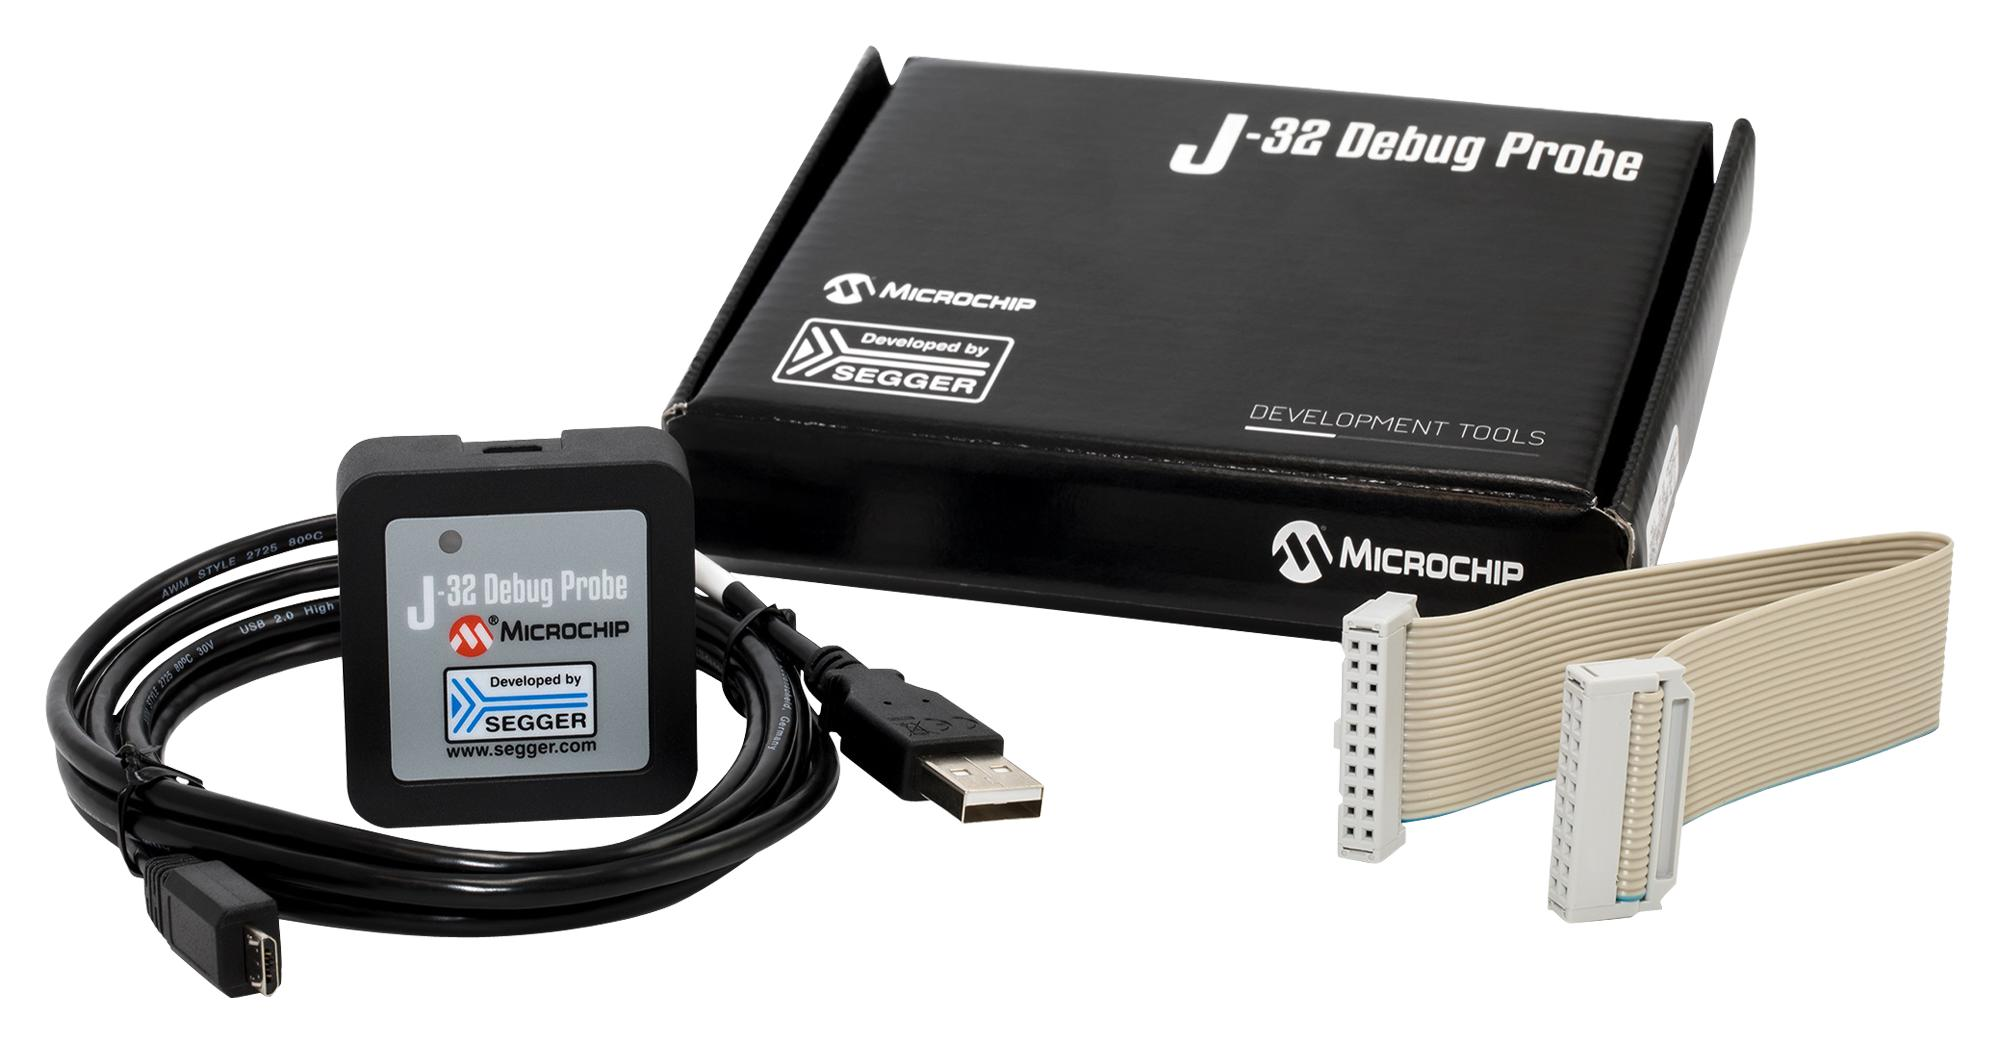
\includegraphics[width=.8\textwidth]{./Figures/segger.jpg}
    \caption{Sonda de depuración \emph{Segger J-32}\protect\footnotemark.}
	\label{fig:sonda}
\end{figure}
\footnotetext{Imagen tomada de \url{https://www.digikey.com/}}

\section{Periféricos de interés}
\label{sec:perifericos}

El dispositivo bajo prueba ofrece una variedad de periféricos para el desarrollo de aplicaciones.
Sin embargo, el cliente manifestó interés solo en los que se nombran a continuación:
\begin{itemize}
    \item CAN: este periférico permite al microcontrolador ser el dispositivo principal en una \emph{Controller Area Network}. La red es de grado industrial y fue diseñada para gestionar una red de sensores en un ambiente automotriz.
    \item PIO: es el puerto de entradas y salidas digitales de propósito general. En el caso del dispositivo bajo prueba, el periférico permite usar circuitos anti rebote, \emph{pull-up} y \emph{pull-down} internos. 
    \item SPI: el periférico permite realizar una conexión del tipo \emph{Serial Peripheral Interface}. Esta conexión es sincrónica y solo apta para distancias cortas.
    \item UART: es un periférico que permite conectarse a puertos y controlar dispositivos serie.
    \item Watchdog: el periférico sirve para detectar un error de ejecución y reiniciar el microprocesador.
\end{itemize}

En la tabla \ref{tab:perifericosresumen} se resume la funcionalidad de cada uno de ellos.

\begin{table}[h]
	\centering
	\caption[Resumen de periféricos]{Resumen de periféricos.}
	\begin{tabular}{l c c}    
		\toprule
        \textbf{Periférico} & \textbf{Funcionalidad}\\
		\midrule
		CAN                 & Bus de comunicación de grado industrial\\        	
		PIO                 & Entradas y salidas digitales\\
		SPI                 & Interfaz de comunicación sincrónica\\
		UART                & Puerto para dispositivos serie\\
		Watchdog            & Detección de errores y reinicio del integrado\\
		\bottomrule
		\hline
	\end{tabular}
	\label{tab:perifericosresumen}
\end{table}

\newpage

\section{Entornos de desarrollo}
\label{sec:entornos}

Para escribir el código que corre en el dispositivo bajo prueba se utilizó un entorno integrado de desarrollo (IDE).
Este IDE es MPLAB y fue provisto por el fabricante del integrado.
MPLAB está compuesto por una colección de programas que trabajan como un único sistema.
Entre ellos se encuentran:

\begin{itemize}
    \item Compilador para lenguaje C.
    \item Biblioteca CMSIS de ARM.
    \item Biblioteca HARMONY 3 de Microchip.
    \item Herramienta gráfica para la planificación de terminales.
    \item Herramienta gráfica para la configuración de periféricos.
    \item Herramienta gráfica para la configuración de reloj.
    \item Cliente GDB para sesiones de depuración.
\end{itemize}

Para realizar el código del inyector por consola de comandos se utilizó el lenguaje de programación Python 3.
Es un lenguaje interpretado que permite escribir código portable.
Además, el intérprete tiene la capacidad de crear ambientes virtuales.
Un ambiente virtual es un espacio de trabajo donde las dependencias instaladas quedan encapsuladas.
De esta manera, se puede simular el despliegue en un ambiente de producción.
Finalmente, junto al intérprete se utilizó un gestor de paquetes llamado PIP.
Esto facilitó la instalación automática del sistema.

Para escribir el código en Python 3, el \emph{firmware} en C y esta memoria en \LaTeX, se utilizó el editor de texto Neovim.
Este programa está basado en el editor Vi de los sistemas Unix.
Su funcionamiento es modal, esto significa que el editor funciona en los siguientes modos:

\begin{itemize}
    \item Modo normal:
        \begin{itemize}
            \item Navegar el documento.
            \item Ejecutar comandos de consola con la posibilidad de volcar el \emph{standard output} en el documento.
            \item Ejecutar \emph{scripts} de Neovim que permiten, por ejemplo, ordenar alfabéticamente una lista.
            \item Ejecutar búsquedas y reemplazos con comandos \emph{sed}.
            \item Grabar y ejecutar macros.
        \end{itemize}
    \item Modo inserción: permite escribir en el documento.
    \item Modo visual: permite seleccionar bloques del documento para aplicar comandos.
    \item Modo terminal: es un \emph{buffer} que emula una terminal Unix.
\end{itemize}

Neovim tiene la capacidad de conectarse a un servidor de análisis sintáctico de un lenguaje en particular.
Esto lo logra a través del \emph{Language Server Protocol (LSP)}.
El protocolo permite que un demonio realice el análisis de la sintaxis del código y envíe al editor información sobre errores y advertencias.
De esta manera se separa al editor del análisis sintáctico del lenguaje.
Además, Neovim tiene incorporado los diccionarios de la mayoría de los idiomas. Con solo ejecutar \texttt{:set spelllang=es} y \texttt{:set spell}, el editor resalta las palabras que no estén escritas en correcto castellano.

El último elemento del flujo de trabajo es el multiplexor de terminal Tmux.
Este programa permite dividir la terminal, crear \emph{buffers} y crear o conectarse a sesiones locales y remotas.
Esto posibilita partir una terminal y trabajar en simultáneo en dos o más ordenadores.
Finalmente, se trabajó de forma integrada con un ambiente de laboratorio remoto y sistemas de desarrollo locales.
En la figura \ref{fig:nvim} se puede ver un ejemplo del flujo de trabajo.

\begin{figure}[htbp]
	\centering
	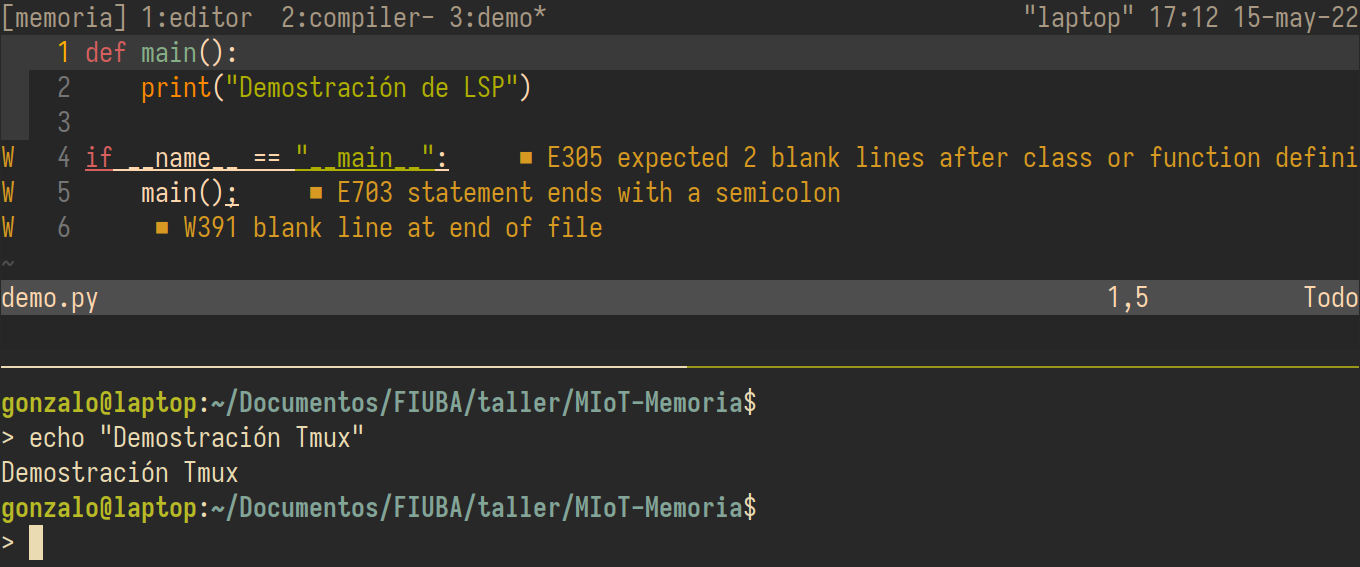
\includegraphics[width=\textwidth]{./Figures/nvimtmux.png}
    \caption{Ejemplo del flujo de trabajo Tmux-Neovim.}
	\label{fig:nvim}
\end{figure}

\newpage

\section{Requerimientos del cliente}
\label{sec:emphuerimientos}

Se realizaron una serie de reuniones con el cliente y se pudo definir los requerimientos del trabajo.
A continuación se enumeran los principales:

\begin{enumerate}
	\item Referentes al inyector por consola de comandos:
		\begin{enumerate}
			\item Generará de una interfaz de usuario.
			\item Permitirá configurar el ensayo a realizar.
			\item Observará la salida del dispositivo bajo prueba.
            \item Inyectará \emph{soft-errors} en el dispositivo bajo prueba.
			\item Persistirá las operaciones, entradas y salidas.
			\item Generará informes del ensayo realizado.
		\end{enumerate}
	\item Referentes al proceso del dispositivo bajo prueba:
		\begin{enumerate}
			\item Verificará el estado de los periféricos del dispositivo bajo prueba.
			\item Detectará si el dispositivo bajo prueba perdió su secuencia.
			\item Generará reportes de estado de periféricos y secuencia.
			\item Permitirá que el inyector por consola de comandos configure el alcance de la secuencia.
			\item Permitirá que el inyector por consola de comandos maneje el flujo de su secuencia.
		\end{enumerate}
\end{enumerate}

El cliente definió algunas restricciones para el desarrollo del sistema.
Estas se enumeran a continuación:

\begin{itemize}
	\item Utilización de un repositorio con control de versiones \emph{Gitlab}.
	\item Documentación del código con \emph{Doxygen}.
	\item Utilización exclusiva del lenguaje de programación \emph{Python 3}.
\end{itemize}

 
	\chapter{Diseño e implementación}
\label{Chapter3}

\definecolor{mygreen}{rgb}{0,0.6,0}
\definecolor{mygray}{rgb}{0.5,0.5,0.5}
\definecolor{mymauve}{rgb}{0.58,0,0.82}

\lstset{ %
  backgroundcolor=\color{white},   % choose the background color; you must add \usepackage{color} or \usepackage{xcolor}
  basicstyle=\footnotesize,        % the size of the fonts that are used for the code
  breakatwhitespace=false,         % sets if automatic breaks should only happen at whitespace
  breaklines=true,                 % sets automatic line breaking
  captionpos=b,                    % sets the caption-position to bottom
  commentstyle=\color{mygreen},    % comment style
  deletekeywords={...},            % if you want to delete keywords from the given language
  %escapeinside={\%*}{*)},          % if you want to add LaTeX within your code
  %extendedchars=true,              % lets you use non-ASCII characters; for 8-bits encodings only, does not work with UTF-8
  %frame=single,	                % adds a frame around the code
  keepspaces=true,                 % keeps spaces in text, useful for keeping indentation of code (possibly needs columns=flexible)
  keywordstyle=\color{blue},       % keyword style
  language=[ANSI]C,                % the language of the code
  %otherkeywords={*,...},           % if you want to add more keywords to the set
  numbers=left,                    % where to put the line-numbers; possible values are (none, left, right)
  numbersep=5pt,                   % how far the line-numbers are from the code
  numberstyle=\tiny\color{mygray}, % the style that is used for the line-numbers
  rulecolor=\color{black},         % if not set, the frame-color may be changed on line-breaks within not-black text (e.g. comments (green here))
  showspaces=false,                % show spaces everywhere adding particular underscores; it overrides 'showstringspaces'
  showstringspaces=false,          % underline spaces within strings only
  showtabs=false,                  % show tabs within strings adding particular underscores
  stepnumber=1,                    % the step between two line-numbers. If it's 1, each line will be numbered
  stringstyle=\color{mymauve},     % string literal style
  tabsize=2,	                   % sets default tabsize to 2 spaces
  title=\lstname,                  % show the filename of files included with \lstinputlisting; also try caption instead of title
  morecomment=[s]{/*}{*/}
}

Este capítulo detalla la generación de contenido original del trabajo.
Se explica su diseño y producción.

\section{Autoevaluación del dispositivo bajo prueba}
\label{sec:autoevaluacion}

La construcción del \emph{firmware} de autoevaluación del dispositivo bajo prueba requirió superar las siguientes etapas:
\begin{itemize}
    \item Configuración de las señales de reloj.
    \item Selección y configuración de los periféricos.
    \item Selección y configuración de los terminales externos.
    \item Implementación de las estrategias de validación de periféricos.
    \item Integración de una secuencia de validación y reporte.
\end{itemize}

Para configurar las frecuencias de reloj se buscó obtener 150 MHz para suministrar al \emph{Master CAN Bus}.
Con esta condición satisfecha, se pudo configurar las frecuencias de reloj del resto de los periféricos.
En la figura \ref{fig:clock} se puede observar la utilización del \emph{Programmable Clock Controller} número cinco.

\begin{figure}[htbp]
	\centering
	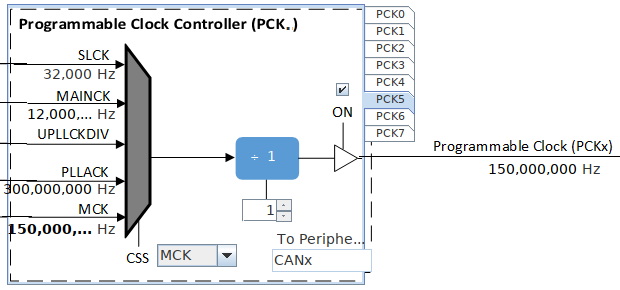
\includegraphics[width=\textwidth]{./Figures/Clock.png}
    \caption{Diagrama de configuración de las señales de reloj.}
	\label{fig:clock}
\end{figure}

El siguiente paso en la etapa de diseño fue la selección de las instancias de los periféricos del integrado.
Es posible que dos periféricos compartan parte del circuito interno o terminales del encapsulado.
Esta situación puede generar una disminución en las funcionalidades o una total incompatibilidad.
Finalmente, se seleccionaron instancias completamente disjuntas.

Luego de seleccionar las instancias de los periféricos, se configuraron para realizar un \emph{loopback}.
La configuración se realizó de la siguiente manera:

\begin{itemize}
    \item \emph{CAN}: se utilizó el \emph{MCAN1} con una configuración de \emph{loopback} interna, como se puede ver en la figura \ref{fig:canloopback}.
    \item \emph{PIO}: se configuraron dos terminales del dispositivo bajo prueba.
        El primero como salida sin \emph{latch} y el segundo como entrada sin circuito anti rebote.
    \item \emph{SPI}: la configuración elegida fue por defecto ya que el \emph{loopback} se logró conectando \emph{TX} y \emph{RX} con un cable.
    \item \emph{UART}: se configuró el periférico con una velocidad de 9600 baudios, 8 bits de datos y sin bits de paridad.
    \item \emph{Watchdog}: el disparo se configuró con un contador en 4095 cuentas.
        Este valor se estimó entre dos y cinco ejecuciones del \emph{loop} principal.
\end{itemize}

\begin{figure}[htbp]
	\centering
	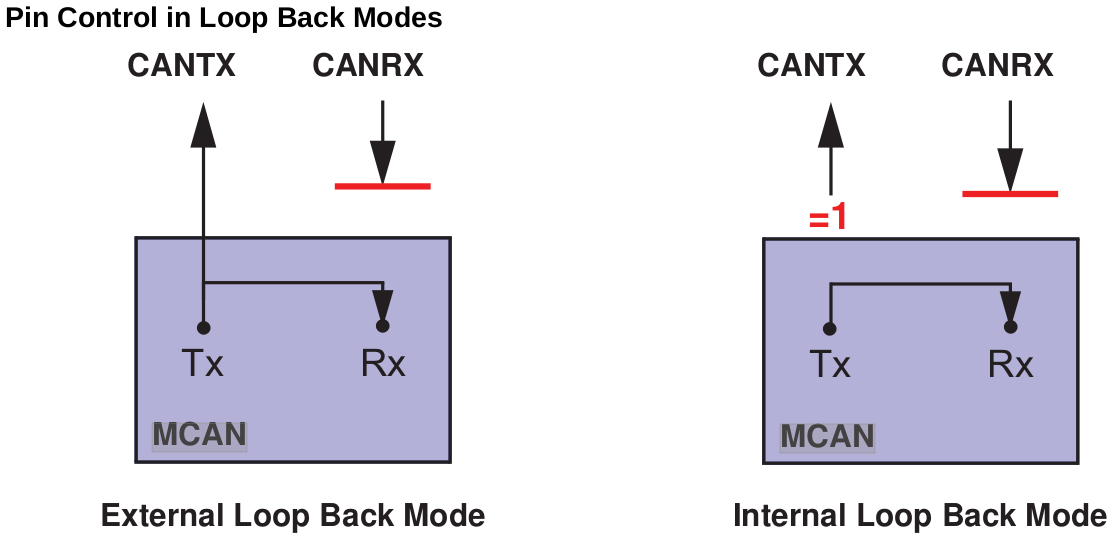
\includegraphics[width=0.8\textwidth]{./Figures/canloopback.png}
    \caption{Diagrama de \emph{loopback} del periférico \emph{CAN}\protect\footnotemark.}
	\label{fig:canloopback}
\end{figure}

\footnotetext{Imagen tomada de la hoja de datos del dispositivo bajo prueba \citep{ARTICLE:dutdatasheet}.}

Como se puede ver en la figura \ref{fig:labo}, se priorizaron los \emph{loopbacks} físicos externos.
Cuando esta estrategia no fue posible, se optó por internos provistos por el fabricante.
Finalmente, en los casos que las dos primeras opciones fueron imposibles, se utilizó una estrategia de \emph{software}.
En la tabla \ref{tab:perifericos} se puede ver un resumen de las estrategias aplicadas.

\begin{table}[h]
	\centering
	\caption[Estrategias de depuración]{Comparación entre estrategias de depuración}

	\begin{tabular}{l c c}    
		\toprule
        \textbf{Periférico} & \textbf{Validación}       & \textbf{Detección en un ciclo}\\
		\midrule
		CAN                 & Loopback interno          & Sí\\		
		PIO                 & Loopback externo          & No\\
		SPI                 & Loopback externo          & Sí\\
		UART                & Lógica en firmware        & No\\
		Watchdog            & Lógica en inyector        & No\\
		\bottomrule
		\hline
	\end{tabular}
	\label{tab:perifericos}
\end{table}

\begin{figure}[htbp]
	\centering
	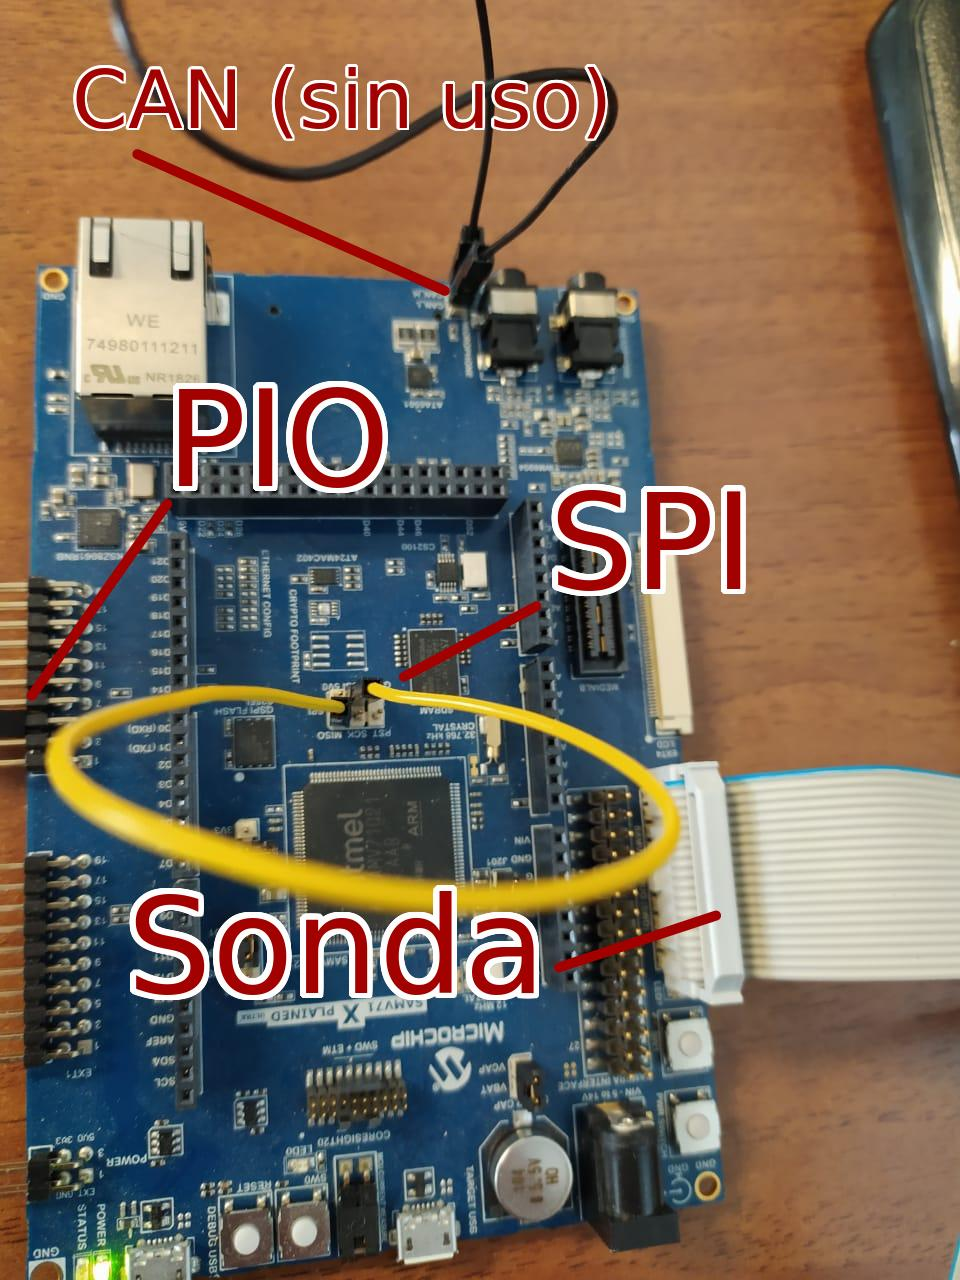
\includegraphics[width=\textwidth]{./Figures/labo.jpeg}
    \caption{Fotografía del dispositivo bajo prueba.}
	\label{fig:labo}
\end{figure}

\newpage

Una vez configurados los componentes de \emph{hardware} del dispositivo bajo prueba; se procedió a diseñar el \emph{firmware}.
Se comenzó con la estructura que define los reportes de estado del dispositivo bajo prueba.
Los reportes están formados por 2 bytes, el primero es el carácter ``F'' y marca el inicio del reporte mientras que el segundo byte lleva la información del estado de los periféricos.
En el código \ref{cod:structs} se puede ver la implementación del segundo byte del reporte.

\begin{lstlisting}[language=C,label=cod:structs,caption=Definición de la estructura de reportes.]  % Start your code-block

#define BIT 1

struct status_bitfield_t
{
    uint8_t CAN:BIT;
    uint8_t SPI:BIT;
    uint8_t PIO:BIT;
    uint8_t WATCHDOG:BIT;
}__attribute__((packed));

typedef union
{
    struct status_bitfield_t status_of;
    uint8_t packed;
}report_t;

\end{lstlisting}

En el código \ref{cod:loop} se puede observar la implementación del lazo principal.
Es importante notar que en la línea 10 se utilizó la \emph{union} para transformar el reporte en caracteres legibles para una persona.
En la figura \ref{fig:firmwareflow} se puede observar el flujo completo del programa.

\begin{lstlisting}[language=C,label=cod:loop,caption=Lazo principal del \emph{firmware} de autoevaluación.]  % Start your code-block

while ( true )
{
    SYS_Tasks ( );
    report.status_of.CAN = validate_CAN();
    report.status_of.PIO = validate_PIO();
    report.status_of.SPI = validate_SPI();
    report.status_of.WATCHDOG = NORMAL;
    
    buffer[FRAME_START] = 'F';
    buffer[FLAGS_INDEX] = report.packed + 'A';
    USART1_Write(&buffer[0], FRAME_SIZE);
    
    WDT_Clear();
}

\end{lstlisting}

\begin{figure}[htbp]
	\centering
	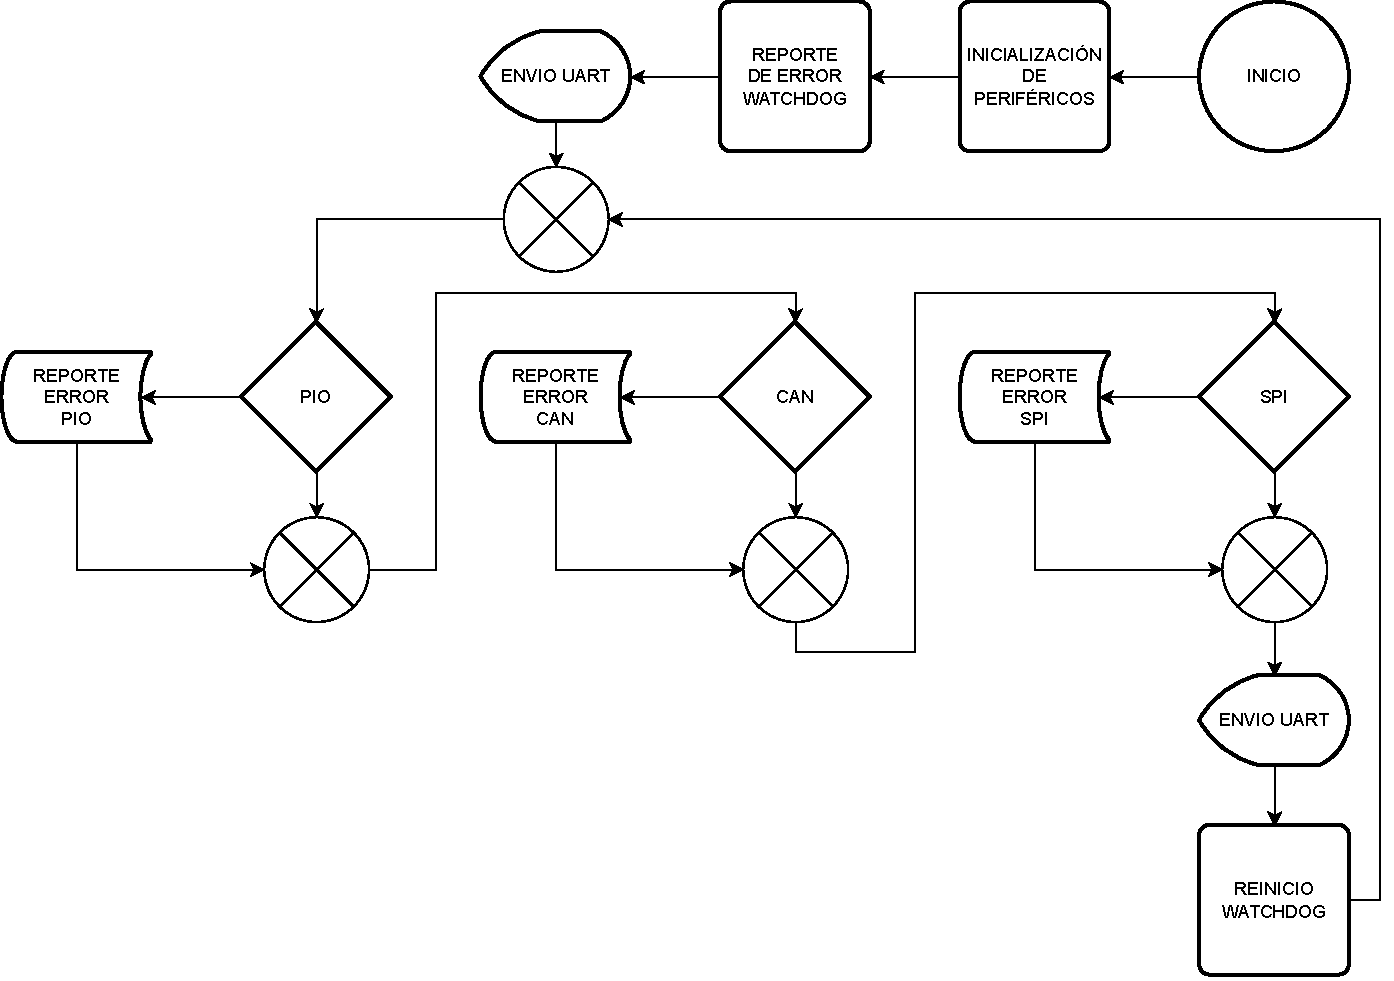
\includegraphics[width=\textwidth]{./Figures/firmwareflow.pdf}
    \caption{Flujo del \emph{firmware} de autoevaluación.}
	\label{fig:firmwareflow}
\end{figure}

\newpage

\section{Interfaz de programación de aplicaciones}
\label{sec:api}

% técnica RAII
% conexión como recurso
La interfaz de programación de aplicaciones tiene la función de abstraer al inyector de errores del servidor \emph{OCD}.
Esto se logró con los siguientes paradigmas y patrones de diseño:

\begin{itemize}
    \item Programación orientada a objetos \emph{(OOP)}: este paradigma de diseño se basa en agrupar en una unidad lógica las funcionalidades y estados que tengan un alto grado de acoplamiento.
        Esto significa que la funciones que tienen efectos colaterales junto a los datos mutados se encapsulan dentro de una construcción denominada objeto.
        Entonces, el principal objetivo de un objeto es contener dentro suyo los efectos colaterales.
        Además, el lenguaje de programación \emph{Python 3} permite, a través de una \emph{class}, modelar un tipo de dato para instanciar a un objeto.
        Finalmente, este patrón se utilizó para contener las funciones de lectura y escritura de registros y memorias.
    \item \emph{Resource Acquisition Is Initialization (RAII)}: este patrón de diseño consiste en modelar el ciclo de vida de un recurso con la implementación de un objeto.
        Un recurso es todo aquello que requiera mantenimiento luego de su uso, como por ejemplo: liberar memoria, cerrar una conexión o unir dos hilos de un programa.
        Esto se logra al adquirir un recurso cuando se invoca el constructor de una \emph{class}, por ejemplo, la conexión con la sonda de depuración se realiza durante la instanciación de un objeto llamado conexión.
        Luego, cuando se desea cerrar la conexión se invoca al destructor del objeto.
        Dentro de esta función se encuentra el código para cerrar de forma ordenada la conexión con la sonda y el dispositivo bajo prueba.
        Finalmente, este patrón de diseño hace que el programa maneje de forma robusta los recursos ya que está garantizada la ejecución de los destructores.
\end{itemize}

En el código \ref{cod:halted} se puede observar un ejemplo de \emph{RAII} donde se maneja como recurso la detención del núcleo del dispositivo bajo prueba.
Esto permite que frente a una excepción del proceso que esté utilizando la interfaz de programación de aplicaciones, el núcleo pueda continuar operando.
Finalmente, se posibilita recuperar el proceso sin tener que reiniciar el dispositivo bajo prueba.

\begin{lstlisting}[language=Python,label=cod:halted,caption=Ejemplo de \emph{Resource Acquisition Is Initialization (RAII)}.]  % Start your code-block

class Halted():
    def __init__(self, target):
        self.target = target

    def __enter__(self):
        self.target.halt()

    def __exit__(self, exc_type, exc_val, traceback):
        self.target.resume()

\end{lstlisting}

Los patrones de diseño utilizados permiten escribir funciones expresivas y robustas.
Como se puede ver en el código \ref{cod:haltedexample}, es fácil comprender lo que sucede.
En la línea 2 se detiene el núcleo y en la línea 3 se lee una posición de memoria.
Luego, en la línea 4 el núcleo reanuda su funcionamiento y finalmente, se retorna el valor leído.

\newpage

\begin{lstlisting}[language=Python,label=cod:haltedexample,caption=Ejemplo de uso de \emph{RAII}.]  % Start your code-block

def readMemory(self, addr: int):
    with Halted(self.target):
        val = self.target.read_memory(addr)
    return val

\end{lstlisting}

En la tabla \ref{tab:funcionalidades} se puede observar un resumen de las funcionalidades y sus estrategias de abstracción.

\begin{table}[h]
	\centering
	\caption[Funcionalidades abstraidas]{Funcionalidades abstraídas}

	\begin{tabular}{l c c}    
		\toprule
        \textbf{Funcionalidad}     & \textbf{Patrón de diseño} & \textbf{Acceso}\\
		\midrule
		Conexión al integrado      & RAII                      & Público\\		
		Detener el núcleo          & RAII                      & Privado\\
		Registros CORE: read/write & OOP                       & Público\\
		Memoria SDRAM: read/write  & OOP                       & Público\\
		\bottomrule
		\hline
	\end{tabular}
	\label{tab:funcionalidades}
\end{table}

Finalmente, se logró abstraer el ciclo de vida de la sesión de depuración que se muestra en la figura \ref{fig:debugsession}.

\begin{figure}[htbp]
	\centering
	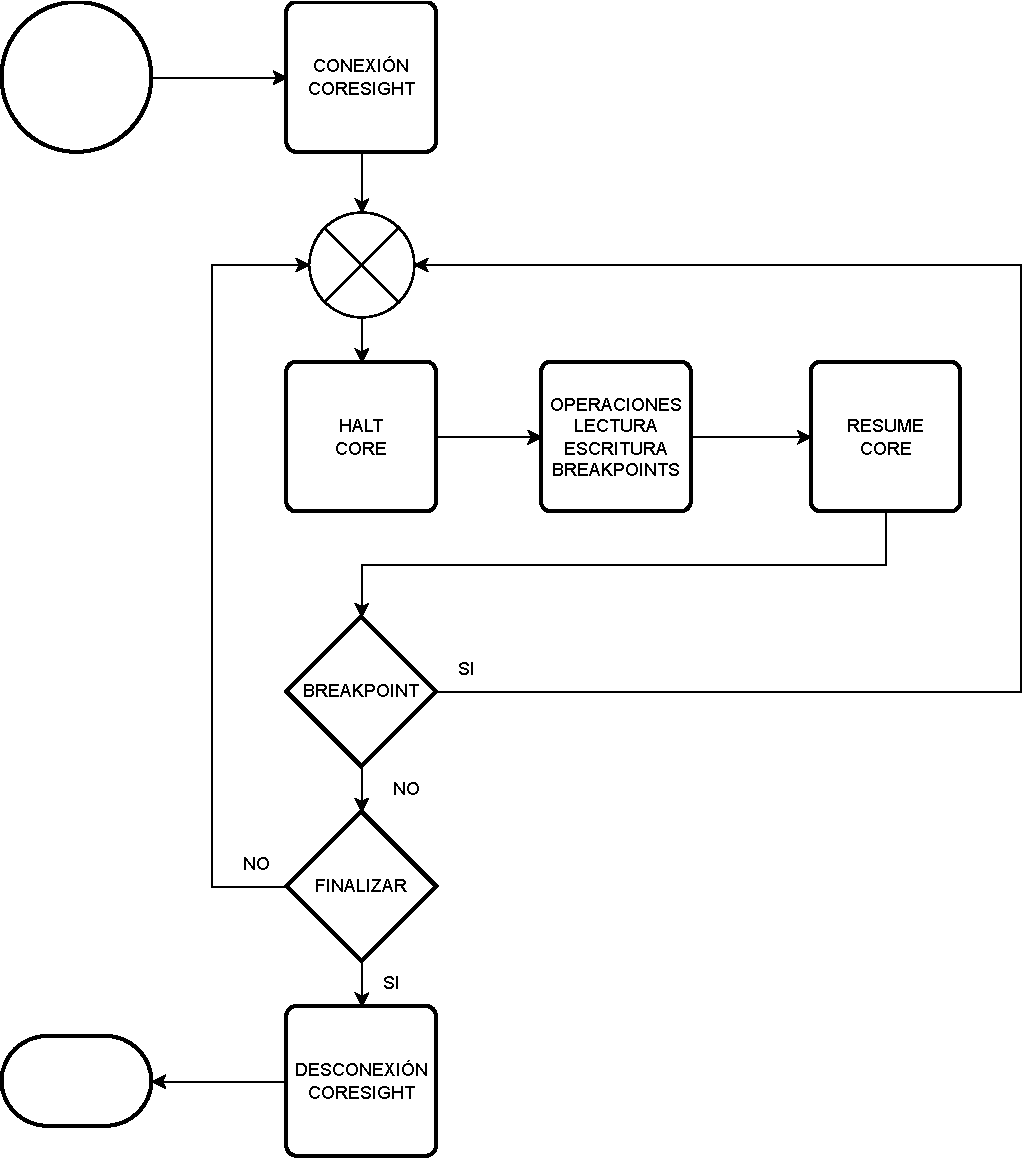
\includegraphics[width=0.9\textwidth]{./Figures/debugsession.pdf}
    \caption{Flujo de una sesión de depuración.}
	\label{fig:debugsession}
\end{figure}

\section{Sistema de inyección de \emph{soft-errors}}
\label{sec:sise}

Una vez lograda la interfaz de programación de aplicaciones explicada en la sección \ref{sec:api}, se pudo construir el inyector por consola de comandos que se muestra en la figura \ref{fig:siseblocks}.
Para lograr que el usuario utilice el programa se creó un sistema de archivo de configuración y un cliente de terminal en texto plano.
El archivo de configuración se genera en formato \emph{YAML} y se encarga de:

\begin{itemize}
    \item Definir si el controlador de ensayos debe recoger los reportes del dispositivo bajo prueba.
    \item Configurar el puerto serie del ordenador.
    \item Definir la simulación:
        \begin{itemize}
            \item El tipo de distribución para usar en el planificador de ensayos.
            \item La tasa de inyección de errores.
            \item La duración del tiempo de exposición en un registro o posición de memoria.
            \item La secuencia de exposición de los registros.
        \end{itemize}
\end{itemize}

% Configuración

En el código \ref{cod:yaml} se puede observar un archivo de configuración.
En particular, la configuración que el sistema ofrece como ejemplo al usuario.
Es importante notar que no se hace referencia a la sesión de depuración.
Finalmente, el ensayo se expresa en términos de parámetros de radiación.

Para facilitar la tarea del usuario, una vez instalado el sistema no es necesario trabajar en una carpeta en particular.
El inyector se puede invocar desde cualquier sitio donde el intérprete de Python 3 tenga permisos de ejecución.
El operador puede entonces crear una carpeta del ensayo.
Luego, crear un archivo de configuración y lanzar desde allí mismo la secuencia de inyecciones.
Finalmente, el sistema genera el reporte correspondiente en esa ruta.

\begin{lstlisting}[language=Python,label=cod:yaml,caption=Ejemplo de configuración de ensayo.]  % Start your code-block

# Perfil determina el tipo de ensayo a realizar
# 'simulador' solo genera inyecciones mientras
# que 'evaluador' recoge y procesa los
# reportes del DUT.
Perfil: 'simulador'

# Interfaz define el puerto serie donde se
# conecto el DUT.
Interfaz:
  puerto: '/dev/ttyACM0'
  baudios: 9600

# Simulacion define la forma de inyectar errores
Simulacion:
  distribucion: 'Poisson'
  tasa: 0.5
  duracion: 5
  registros: 'secuencial'

\end{lstlisting}

% Consola

La interfaz por consola se logró al utilizar el \emph{standar input} y el \emph{standar output} del proceso padre.
En el caso de una sesión iniciada por un humano, el emulador de terminal del sistema.
En una primera iteración de la consola se realizó una interfaz ASCII con la biblioteca \emph{curses}.
Sin embargo, el cliente prefirió una interfaz por texto plano para facilitar el \emph{parsing} de un sistema de integración continua.
En particular, el módulo de \emph{CI/CD} de \emph{Gitlab}.

El usuario invoca el programa al ejecutar el comando \texttt{sise}.
Luego la consola responde con la leyenda \texttt{Ingrese el archivo de configuración > }.
Se escribe la ruta y nombre del archivo a utilizar y el sistema lanza el ensayo.
El reporte generado se persiste en la carpeta donde se inició el programa.

% Planificador de ensayos

Con la información suministrada por el archivo de configuración y la consola, se puede iniciar el planificador de ensayos.
Este módulo tiene la función de generar una variable aleatoria que genera tiempos entre inyecciones de errores.
La variable aleatoria se construye con los datos de distribución y tasa de error.
El proceso aleatorio se repite hasta que la sumatoria de los tiempos generados sea igual o mayor al tiempo deseado del ensayo.
Luego, se asigna cada tiempo a un registro del núcleo en particular.
Esta asignación se realiza según la configuración del usuario.
Finalmente, se entrega la planificación al controlador de ensayos.

% Controlador de ensayos

El controlador de ensayos es un hilo del programa que tiene la misión de ejecutar una planificación de ensayos.
Su ejecución se basa en la interfaz de abstracción de aplicaciones explicada en la sección \ref{sec:api}.
Luego, tiene la responsabilidad de observar el tiempo de ejecución del dispositivo bajo prueba.
Cuando el momento es adecuado, el controlador invoca una función de \emph{bit flip}.
El bit a invertir se determina en el momento de inyección con una variable aleatoria uniforme.
Finalmente, cuando el controlador consume la totalidad de la planificación, envía una señal para solicitar el \emph{join} con el hilo principal del programa.

% Generador de reportes

El generador de reportes es un hilo que escucha el puerto serie del ordenador.
Mientras dura el ensayo, almacena todos los mensajes entrantes y los acumula junto a un \emph{timestamp}.
De la misma manera, persiste las inyecciones realizadas como tuplas.
Estas tuplas tienen todos los datos relevantes de la inyección junto a un \emph{timestamp}.
Cuando el ensayo finaliza, recibe una señal desde el hilo principal del programa que le ordena hacer un \emph{join}.
Luego, el generador de reportes deja de escuchar el puerto serie y al controlador de ensayos.
Seguidamente, se procede a construir un reporte en formato de tabla de \emph{MS Excel} y \emph{CSV}.
Para lograrlo, se genera una relación de causalidad entre errores inyectados y respuestas del dispositivo bajo prueba.
Finalmente, se generan los archivos en la carpeta donde el comando \texttt{sise} fue lanzado.

% Funcionamiento concurrente

La mayor dificultad del inyector fue el manejo concurrente de los hilos del controlador de ensayo y el generador de reportes.
En particular, porque ambos hilos comparten el uso del puerto serie.
Esta situación genera una condición de carrera que se tuvo que manejar.
Luego, se decidió evitar candados y semáforos al explotar la topología de \emph{bus} en árbol del protocolo \emph{USB}.
De esta manera, la conexión con la UART y el DAP se trató como si estuviesen conectados en puertos físicos diferentes.
Esta decisión de diseño tiene la ventaja de no incrementar el error de las mediciones de tiempo.
Un error en la medición generaría relaciones de causalidad incorrectas y por lo tanto los informes no serían confiables.
Sin embargo, se introdujo un punto de falla al depender de la capacidad de la sonda de depuración y su gestión de su árbol de dispositivos.
Finalmente, en la figura \ref{fig:concurrencia} se puede observar un diagrama con los hilos del programa.

\begin{figure}[htbp]
	\centering
	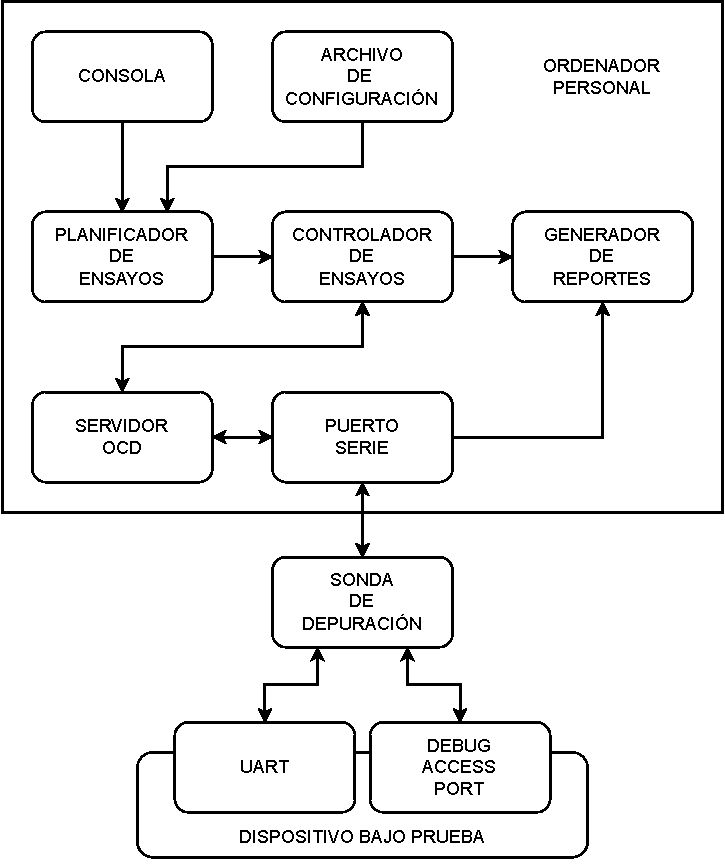
\includegraphics[width=\textwidth]{./Figures/siseblocks.pdf}
    \caption{Diagrama en bloques del sistema de inyección de soft-errors.}
	\label{fig:siseblocks}
\end{figure}

\begin{figure}[htbp]
	\centering
	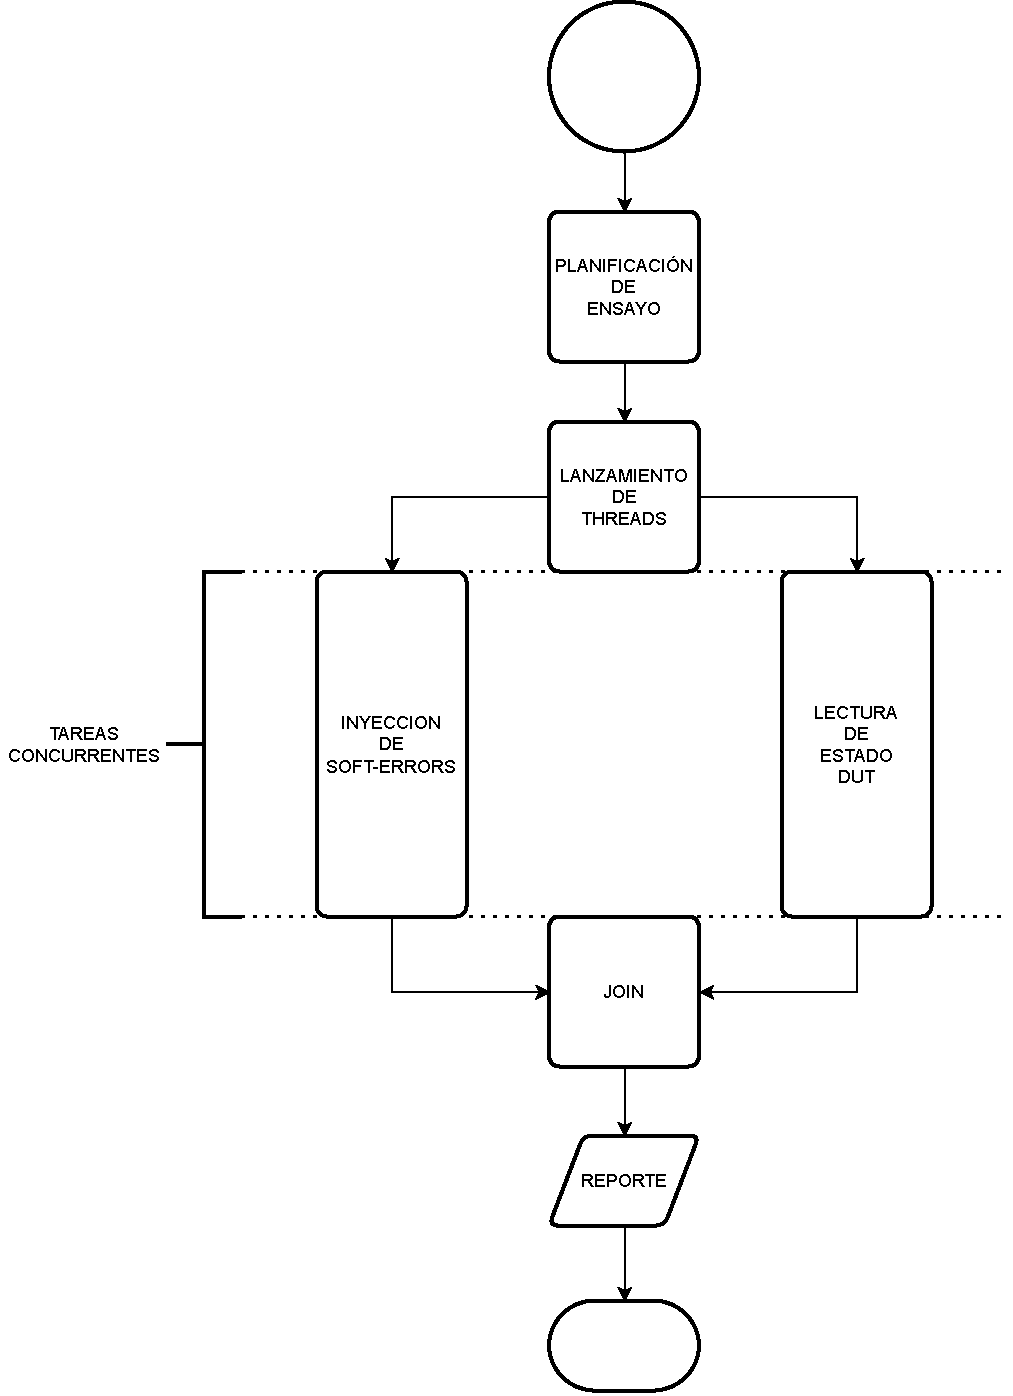
\includegraphics[width=\textwidth]{./Figures/concurrencia.pdf}
    \caption{Flujo de tareas concurrentes.}
	\label{fig:concurrencia}
\end{figure}

\section{Biblioteca para el desarrollo de ensayos}
\label{fig:biblioteca}

Para que el usuario pueda realizar sus propios ensayos, se creó una biblioteca que le provee la funcionalidad necesaria.
Esta biblioteca se divide en dos partes:

\begin{itemize}
    \item Funcionalidades del núcleo.
    \item Funcionalidades de la memoria.
\end{itemize}

Para facilitar la interacción con el núcleo se implementó una lista con los nombres de los registros.
De esta manera, se facilita el uso de las funciones.
En el código \ref{cod:corereg} se puede observar la colección que se le ofrece al diseñador.

\begin{lstlisting}[language=Python,label=cod:corereg,caption=Lista de registros accesibles por el usuario.]  % Start your code-block

CORE_REGISTERS = [
    'lr', 'pc', 'sp', 'xpsr', 'r0', 'r1', 'r2', 'r3',
    'r4', 'r5', 'r6', 'r7', 'r8', 'r9', 'r10', 'r11', 'r12'
]

\end{lstlisting}

Las funcionalidades ofrecidas para manipular el núcleo del integrado se muestran en el código \ref{cod:coreapi}.
Los detalles son los siguientes:

\begin{itemize}
    \item En la línea 6 se muestra el uso de la función de lectura de registros.
        Se invoca a partir del objeto de conexión y su argumento es el nombre del registro a leer.
    \item En la línea 10 se puede observar el uso del método de escritura de registros.
        Necesita como argumento el nombre del registro y el valor a escribir.
        Luego, la función retorna una tupla con los valores previos y posteriores a la escritura.
    \item En la línea 15 se ve una llamada a la función de \emph{bit flip} del registro del núcleo.
        Se debe indicar el nombre del registro y la posición del bit a invertir.
        Finalmente, se retorna el valor previo y posterior al llamado del método.
\end{itemize}

\newpage

\begin{lstlisting}[language=Python,label=cod:coreapi,caption=Ejemplo de uso en registros del núcleo.]  % Start your code-block

import sise.library as sise

dut = sise.Connection()

# Lectura del registro del CORE
rreg = dut.readRegister('pc')
print("PC:", rreg)

# Escritura del registro del CORE
wreg = writeRegister('r0', 0xffffffff)
print("(old, new):", wreg)

# Bit-flip en registro del CORE
bit = 2
bfreg = bitFlipRegister('r1', bit)
print("(old, new):", bfreg)

del(dut)

\end{lstlisting}

Para interactuar con la memoria se dispone de las funciones demostradas en el código \ref{cod:menapi}.
Los métodos se detallan a continuación:
\begin{itemize}
    \item Línea 7: el método permite realizar una lectura del dato en una posición de memoria.
        El argumento es una dirección alineada de la memoria y el retorno es el valor de una palabra de 32 bits.
    \item Línea 12: esta función se utiliza para escribir una posición alineada de memoria.
        Se necesita pasarle una dirección y un valor a escribir.
        Finalmente, retorna una tupla con el dato previo y posterior a la ejecución del método.
    \item Línea 18: la subrutina posibilita hacer un \emph{bit flip} en una posición de memoria.
        El método toma como argumento una posición alineada de memoria y el bit a invertir.
        Luego de su ejecución, se retorna el valor previo y posterior a la inversión.
\end{itemize}

\begin{lstlisting}[language=Python,label=cod:menapi,caption=Ejemplo de uso en memoria.]  % Start your code-block

import sise.library as sise

dut = sise.Connection()

# Lectura de memoria
addr = 0x20400004
rmen = readMemory(addr)
print("men:", rmen)

# Escritura de memoria
addr = 0x20400008
wmen = writeMemory(addr, 0xfafafafa):
print("(old, new):", wmen)

# Bit-flip en memoria
addr = 0x20400000
bit = 0
bfmen = dut.bitFlipMemory(addr, bit)
print("(old, new):", bfmen)

del(dut)

\end{lstlisting}

	% Chapter Template

\chapter{Ensayos y resultados} % Main chapter title

\label{Chapter4} % Change X to a consecutive number; for referencing this chapter elsewhere, use \ref{ChapterX}

En este capítulo se describe la estrategia de pruebas adoptada para determinar que el sistema se comporta de forma esperada.

%----------------------------------------------------------------------------------------
%	SECTION 1
%----------------------------------------------------------------------------------------

\section{Laboratorio remoto}
\label{sec:lab}

Durante las primeras etapas del desarrollo no se disponía en Buenos Aires del dispositivo bajo prueba.
Por esta razón, se montó un laboratorio remoto en San Carlos de Bariloche.
Se dispuso una placa de evaluación \emph{SAM V71 Xplained Ultra} conectada a un ordenador dentro de la red de INVAP S.E.
La conexión entre la placa y el ordenador se logró a través de una sonda de depuración \emph{Segger J-32}.

Para poder acceder al laboratorio remoto que se muestra en la figura \ref{fig:remotelab} se necesitó:

\begin{itemize}
    \item Credenciales de acceso y conexión a la VPN de INVAP S.E.
    \item Crear un túnel SSH con el ordenador remoto.
\end{itemize}

El túnel SSH se generó con \emph{X11 forwarding} habilitado.
De esta manera, se pudo generar ventanas gráficas en el ambiente local.
Además, las operaciones de consola se integraron al ordenador personal con una sesión de Tmux.
Finalmente, se logró implementar una interfaz de control del laboratorio remoto con una apariencia idéntica al ambiente local.

\begin{figure}[htbp]
	\centering
	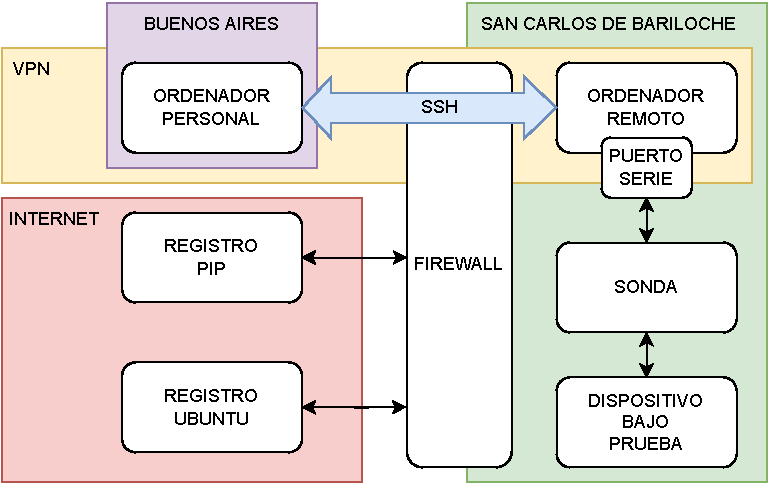
\includegraphics[width=\textwidth]{./Figures/vpn.pdf}
    \caption{Diagrama en bloques del laboratorio remoto.}
	\label{fig:remotelab}
\end{figure}

Para poder instalar las dependencias y los servidores OCD evaluados, se habilitaron los puertos necesarios que permitieron al ordenador remoto conectarse a los recursos en la Internet.
Sin embargo, algunos recursos debieron ser compilados en el \emph{host} y la transferencia de los \emph{tarballs} se realizó por medio de \emph{Secure Copy Files (scp)}.

Con el laboratorio remoto montado, se procedió a realizar las siguientes pruebas:
\begin{itemize}
    \item Pruebas de configuración de sondas de depuración y compatibilidad con servidores OCD.
    \item Pruebas de acceso al dispositivo bajo prueba.
\end{itemize}

Las pruebas referidas a la sonda de depuración arrojaron como resultado lo siguiente:

\begin{itemize}
    \item El modo de \emph{boot} de la sonda determina el nivel de acceso al dispositivo bajo prueba.
    \item Para lograr inyecciones de \emph{soft-errors} la sonda de depuración debe poder iniciar en modo \emph{CMSIS-DAP}.
    \item Si la sonda de depuración no se encuentra en modo \emph{CMSIS-DAP}, \emph{PyOCD} solo puede realizar escritura en la memoria \emph{flash}.
    \item Cambiar de modo una sonda de depuración requiere reiniciarla.
        Por lo tanto, no es factible realizar cambios de configuración luego de iniciado un ensayo.
\end{itemize}

Las pruebas referidas al acceso al dispositivo bajo prueba tuvieron los siguientes resultados:

\begin{itemize}
    \item Si no se dispone de un \emph{Device Family Pack (DFP)}, \emph{PyOCD} se conecta al dispositivo bajo prueba y lo identifica como \emph{Generic Cortex-M}.
    \item Bajo la identificación de \emph{Generic Cortex-M} se puede acceder a todos los registros de núcleo.
    \item Bajo la identificación de \emph{Generic Cortex-M} se puede acceder a la memoria \emph{SDRAM} y reconoce como error una posición desalineada.
    \item Bajo la identificación de \emph{Generic Cortex-M} se puede acceder a otras direcciones del integrado solo en modo lectura.
        Si se intenta ingresar en modo escritura no sucede ningún cambio pero el servidor OCD no responde con un error.
        Su respuesta es de operación exitosa, pero no se manifiestan cambios.
\end{itemize}

PyOCD posee un módulo de búsqueda y descarga de DFP, sin embargo, su funcionamiento no es confiable y genera una excepción durante su ejecución.
Se intentó verificar su funcionamiento en otras plataformas y se pudo observar que su desarrollo fue realizado en el lenguaje de programación \emph{Rust}.
Este módulo hizo imposible instalar el servidor OCD en una \emph{single board computer}.
Dado que, su compilador consume una cantidad de memoria que supera el \emph{hardware} disponible en placas como \emph{Raspberry Pi 4B}.
Se pudo verificar que este es el único módulo escrito en \emph{Rust}, pero no es posible desacoplarlo del servidor OCD.
Finalmente, PyOCD tiene una limitación de plataformas compatibles que podría ser sorteada con \emph{cross} compilación.

La única dificultad en el uso del laboratorio remoto se presentó en las pruebas de la sonda de depuración.
Muchas de las pruebas requirieron reiniciar la sonda y esto solo es posible al desconectar el cable \emph{USB}.
La operación debió ser realizada por el co-director de este trabajo.
En la tabla \ref{tab:funcionalidades}, se puede ver un resumen de las funcionalidades del laboratorio remoto.
Las funcionalidades con tres marcas tienen el mismo nivel de servicio que el laboratorio local, las de dos marcas tienen un nivel algo inferior y las que tienen solo una marca tienen un nivel de servicio bajo.

\begin{table}[h]
	\centering
	\caption[Resumen del laboratorio remoto]{Resumen del laboratorio remoto.}

	\begin{tabular}{l c}    
		\toprule
        \textbf{Funcionalidad}             & \textbf{Nivel de servicio} \\
		\midrule
		Carga de binarios en DUT           & ++  \\		
		Comunicación con registro PIP      & +++ \\
		Comunicación con registro Ubuntu   & +++ \\
		Comunicación con debug access port & +++ \\
		Comunicación con UART              & +   \\
		\bottomrule
		\hline
	\end{tabular}
	\label{tab:funcionalidades}
\end{table}

\section{Ensayos de inyector}
\label{sec:testinyector}

El inyector de \emph{soft-errors} se sometió a ensayos en los siguientes ambientes:

\begin{itemize}
    \item Laboratorio remoto.
    \item Laboratorio local.
    \item Dispositivo alternativo \emph{NUCLEO-F429ZI}.
        Este último ambiente se puede ver en la figura \ref{fig:alternativo} y se utilizó para probar si el inyector es genérico.
        En particular, porque utiliza una sonda de depuración distinta.
\end{itemize}

\begin{figure}[htbp]
	\centering
	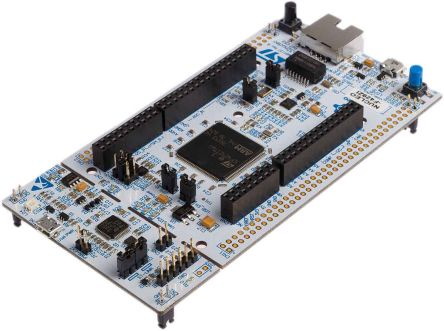
\includegraphics[width=0.8\textwidth]{./Figures/alternativo.jpg}
    \caption{Dispositivo alternativo \emph{NUCLEO-F429ZI}.}
	\label{fig:alternativo}
\end{figure}

Se generaron múltiples archivos de configuración para definir distintos casos de prueba.
Luego, se corrieron los ensayos en los tres ambientes y se compararon los resultados.
Además, se usó una variante adicional en el dispositivo alternativo.
Se probó el comportamiento del inyector sobre un blanco con \emph{mbedOS}.
Finalmente, en la tabla \ref{tab:resensayos} se puede observar un resumen de los resultados obtenidos.
En la tabla se marca con tres cruces los ensayos que arrojaron resultados sobresalientes, con dos cruces los ensayos que mostraron inconvenientes mínimos y con una cruz los ensayos con resultados insatisfactorios.

\begin{table}[h]
	\centering
	\caption[Resumen de ensayos]{Resumen de ensayos}

	\begin{tabular}{l c c c}    
		\toprule
        \textbf{Ensayo}                 & \textbf{Lab. local} & \textbf{Lab. remoto} & \textbf{DUT alterno} \\
		\midrule
		Escritura SDRAM                 & +++                 & +++                  & +++ \\
		Escritura registros CORE        & +++                 & +++                  & +++ \\
		Funcionalidades extras          & ++                  & ++                   & +++ \\
		Halt CORE                       & +++                 & +++                  & +++ \\
		Lectura SDRAM                   & +++                 & +++                  & +++ \\
		Lectura registros CORE          & +++                 & +++                  & +++ \\		
		Uso concurrente de puerto serie & +++                 & +                    & +++ \\
        Resume CORE                     & +++                 & +++                  & +++ \\
		\bottomrule
		\hline
	\end{tabular}
	\label{tab:resensayos}
\end{table}

El dispositivo alternativo arrojó los mejores resultados porque PyOCD tiene el \emph{Device Family Pack}.
Por otro lado, el laboratorio remoto tuvo malos resultados en las pruebas de concurrencia.
Esto fue así ya que se debía pedir ayuda al personal de INVAP S.E. cada vez que la sonda necesitaba ser reiniciada. 

\section{Validación con el cliente}
\label{sec:validacion}

La etapa final del proceso de pruebas fue una serie de demostraciones realizadas al cliente.
Luego de cada demostración se indicaban las correcciones a realizar.
Seguidamente, se mejoraba el código y se repetía la demostración.
Estos ciclos de iteraciones tenían una frecuencia de 15 días.
Finalmente, se llegó al cumplimiento total de los requerimientos como se puede ver en la tabla \ref{tab:validacion}

\begin{table}[h]
	\centering
	\caption[Resumen de la validación con el cliente]{Resumen de la validación con el cliente}

	\begin{tabular}{l c}    
		\toprule
        \textbf{Expectativas}     & \textbf{Cumplimiento} \\
		\midrule
		Acceso a memoria          & +++                   \\
		Acceso al CORE            & +++                   \\
		Biblioteca de ensayos     & +++                   \\		
		Capacidad de bit-flip     & +++                   \\
		Configuración del sistema & +++                   \\
		Distribución de errores   & +++                   \\
		Validación de periféricos & +++                   \\
        Generación de reportes    & +++                   \\
		\bottomrule
		\hline
	\end{tabular}
	\label{tab:validacion}
\end{table}

En la figura \ref{fig:demobitflip} se puede observar una demostración del acceso a memoria SDRAM.
Se puede ver que la terminal está dividida en las siguientes partes:

\begin{itemize}
    \item Sección izquierda: se hizo una demostración paso a paso.
        Primero, se importó la biblioteca dentro del espacio de trabajo.
        Luego, se conectó al dispositivo y se cargó una dirección de memoria y el bit a invertir.
        Seguidamente, se realizó una inversión y se mostró el valor previo y posterior al \emph{bit flip}.
        Finalmente, se cerró la conexión con el dispositivo alternativo.
    \item Sección derecha: se observa el mapa de memoria SDRAM del dispositivo alternativo.
        Se usó para mostrarle al cliente las direcciones de memoria ensayadas.
\end{itemize}

Este ensayo además de demostrar el acceso a memoria SDRAM también ejercita la capacidad de realizar \emph{bit flip}.
Finalmente, el cliente consideró que se habían cumplido todos los requisitos y que el trabajo se encontraba finalizado.

Los ensayos finales se volvieron a reproducir en presencia de un estudiante de la especialización en sistemas embebidos quién actualmente utiliza la herramienta en el marco de su proyecto final.

\begin{figure}[htbp]
	\centering
	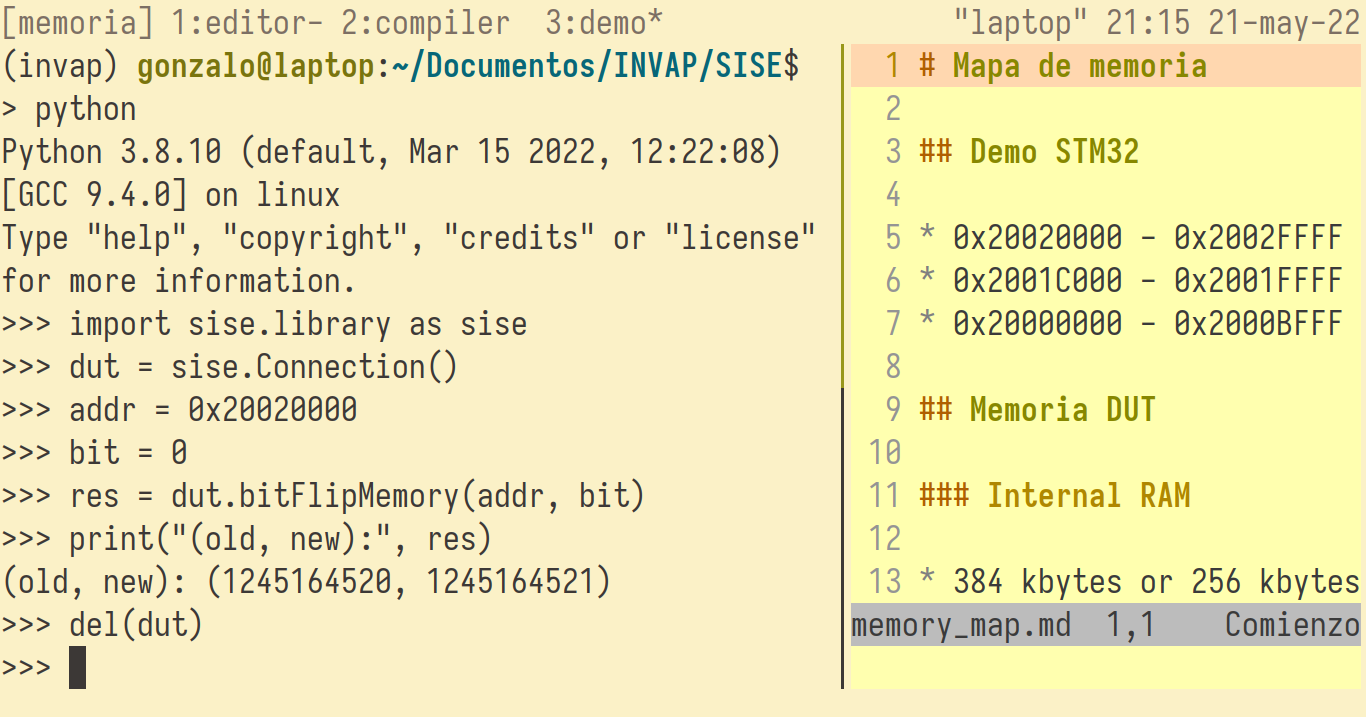
\includegraphics[width=\textwidth]{./Figures/demo_bitflip.png}
    \caption{Demostración de acceso a memoria.}
	\label{fig:demobitflip}
\end{figure}
 
	\chapter{Conclusiones}
\label{Chapter5}

Este capítulo explica de forma breve el cierre del trabajo realizado, sus logros y futuro.

\section{Resultados obtenidos}
\label{sec:5resultados}

El trabajo logró cumplir las expectativas y requerimientos del cliente.
En particular, los siguientes objetivos:

\begin{itemize}
    \item Creación de un sistema de inyección de \emph{soft-errors} que permita evaluar técnicas de mitigación de errores.
    \item Acceso a la memoria volátil del dispositivo bajo prueba.
    \item Biblioteca para el diseño de ensayos en lenguaje \emph{Python 3}.
\end{itemize}

La recepción de este trabajo fue muy positiva; ya que en la actualidad, INVAP S.E. se encuentra en proceso de integrar la herramienta en su ambiente de desarrollo de satélites.
Además, el sistema realizado se utiliza dentro del marco de un proyecto final en la Especialización en Sistemas Embebidos.

\section{Trabajo futuro}
\label{sec:5futuro}

La investigación realizada durante la producción del trabajo sugiere que es posible agregar las siguientes funcionalidades:

\begin{itemize}
    \item Conexión entre el código fuente del dispositivo bajo prueba y el inyector de \emph{soft-errors}.
    \item Creación de instrucciones específicas para la inyección de \emph{single event functional interrupt}.
\end{itemize}
 
\end{verbatim}

Los apéndices también deben escribirse en archivos .tex separados, que se deben ubicar dentro de la carpeta \emph{Appendices}. Los apéndices vienen comentados por defecto con el caracter \code{\%} y para incluirlos simplemente se debe eliminar dicho caracter.

Finalmente, se encuentra el código para incluir la bibliografía en el documento final.  Este código tampoco debe modificarse. La metodología para trabajar las referencias bibliográficas se desarrolla en la sección \ref{sec:biblio}.
%----------------------------------------------------------------------------------------

\section{Bibliografía}
\label{sec:biblio}

Las opciones de formato de la bibliografía se controlan a través del paquete de latex \option{biblatex} que se incluye en la memoria en el archivo memoria.tex.  Estas opciones determinan cómo se generan las citas bibliográficas en el cuerpo del documento y cómo se genera la bibliografía al final de la memoria.

En el preámbulo se puede encontrar el código que incluye el paquete biblatex, que no requiere ninguna modificación del usuario de la plantilla, y que contiene las siguientes opciones:

\begin{lstlisting}
\usepackage[backend=bibtex,
	natbib=true, 
	style=numeric, 
	sorting=none]
{biblatex}
\end{lstlisting}

En el archivo \file{reference.bib} se encuentran las referencias bibliográficas que se pueden citar en el documento.  Para incorporar una nueva cita al documento lo primero es agregarla en este archivo con todos los campos necesario.  Todas las entradas bibliográficas comienzan con $@$ y una palabra que define el formato de la entrada.  Para cada formato existen campos obligatorios que deben completarse. No importa el orden en que las entradas estén definidas en el archivo .bib.  Tampoco es importante el orden en que estén definidos los campos de una entrada bibliográfica. A continuación se muestran algunos ejemplos:

\begin{lstlisting}
@ARTICLE{ARTICLE:1,
    AUTHOR="John Doe",
    TITLE="Title",
    JOURNAL="Journal",
    YEAR="2017",
}
\end{lstlisting}


\begin{lstlisting}
@BOOK{BOOK:1,
    AUTHOR="John Doe",
    TITLE="The Book without Title",
    PUBLISHER="Dummy Publisher",
    YEAR="2100",
}
\end{lstlisting}


\begin{lstlisting}
@INBOOK{BOOK:2,
    AUTHOR="John Doe",
    TITLE="The Book without Title",
    PUBLISHER="Dummy Publisher",
    YEAR="2100",
    PAGES="100-200",
}
\end{lstlisting}


\begin{lstlisting}
@MISC{WEBSITE:1,
    HOWPUBLISHED = "\url{http://example.com}",
    AUTHOR = "Intel",
    TITLE = "Example Website",
    MONTH = "12",
    YEAR = "1988",
    URLDATE = {2012-11-26}
}
\end{lstlisting}

Se debe notar que los nombres \emph{ARTICLE:1}, \emph{BOOK:1}, \emph{BOOK:2} y \emph{WEBSITE:1} son nombres de fantasía que le sirve al autor del documento para identificar la entrada. En este sentido, se podrían reemplazar por cualquier otro nombre.  Tampoco es necesario poner : seguido de un número, en los ejemplos sólo se incluye como un posible estilo para identificar las entradas.

La entradas se citan en el documento con el comando: 

\begin{verbatim}
\citep{nombre_de_la_entrada}
\end{verbatim}

Y cuando se usan, se muestran así: \citep{ARTICLE:1}, \citep{BOOK:1}, \citep{BOOK:2}, \citep{WEBSITE:1}.  Notar cómo se conforma la sección Bibliografía al final del documento. 

	\chapter{Introducción específica}

\label{Chapter2}

En este capítulo se detallan las tecnologías que forman parte del trabajo.
Son productos de terceros que se integran en las herramientas entregadas al cliente.

\section{Arquitectura del dispositivo bajo prueba}
\label{sec:dut}

El trabajo fue realizado para un tipo de microcontrolador específico.
Su diseño forma parte de la familia \emph{Cortex M7} de la empresa \emph{ARM}.
En la figura \ref{fig:cortexm} se puede observar un diagrama en bloques de la arquitectura.

El dispositivo bajo prueba es el microcontrolador \emph{SAM V71} diseñado por la empresa \emph{Atmel} y comercializado por \emph{Microchip}.
El integrado fue pensado para aplicaciones automotrices según el estándar \emph{ISO-TS-16949}.
Además, el circuito puede operar con un reloj de 300 MHz y almacenar un programa de 2048 kB.
Las estructuras de datos del programa pueden aprovechar la memoria cache dual de 16 kB \citep{ARTICLE:dutdatasheet}.
Las principales características del dispositivo bajo prueba son:

\begin{itemize}
    \item Núcleo:
        \begin{itemize}
            \item Unidad de punto flotante de precisión simple y doble.
            \item Unidad de protección de memoria con 16 zonas.
            \item Instrucciones para el procesamiento digital de señales.
        \end{itemize}
    \item Memorias:
        \begin{itemize}
            \item \emph{ROM} de 16 kB con rutinas de inicialización. Esto permite iniciar el sistema desde los periféricos \emph{UART0} y \emph{USB}.
            \item Controlador de memoria estática para el uso de memorias externas.
        \end{itemize}
    \item Sistema:
        \begin{itemize}
            \item Reloj de tiempo real con gestión de calendario gregoriano.
            \item Reinicio por alimentación, detección de caída de tensión y doble \emph{Watchdog}.
            \item Puerto dual de 24 canales para la gestión de acceso a memoria.
            \item Compensación por variaciones de reloj.
        \end{itemize}
\end{itemize}

\newpage

Este integrado fue sometido a una prueba por radiación donde se evaluaron SEE y la calificación de dosis total de ionización (TID).
El microcontrolador mantuvo su funcionamiento en todo el rango de temperatura de calificación militar.
Además, el dispositivo es inmune a \emph{Single Event Latch-up} con una tolerancia de 60,0 $MeV.cm^2/mg$.
Esta sensibilidad fue probada con una cámara de iones pesados.
En cuanto a la calificación de dosis total de ionización, el lote fue sometido a un ensayo de 30 krad(Si) y la prueba fue superada.
Finalmente, los ensayos suministrados por el fabricante permiten concluir que no es necesario realizar inyecciones de errores en la memoria \emph{flash} \citep{ARTICLE:dutrad}.

Al fabricante del dispositivo bajo prueba se le impone respetar el mapa de memoria y registros del núcleo.
Esto permitió construir un inyector de \emph{soft-errors} genérico.
Finalmente, la herramienta entregada funciona para cualquier integrado de la familia \emph{Cortex M}.

\begin{figure}[htbp]
	\centering
	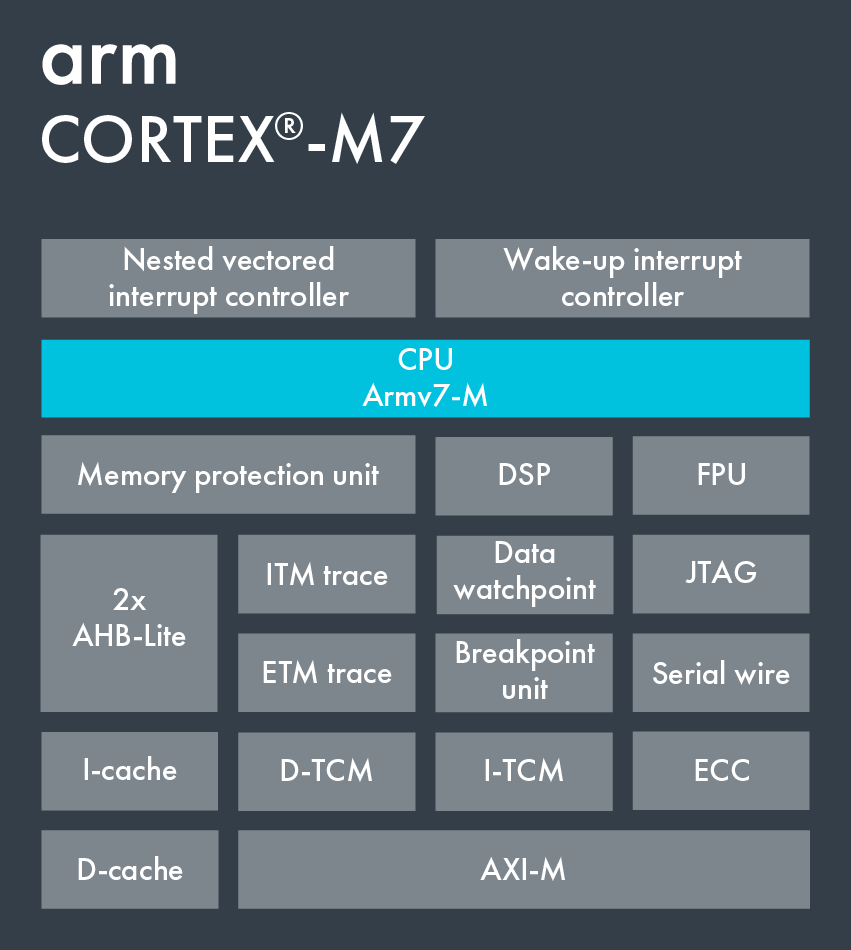
\includegraphics[width=.7\textwidth]{./Figures/Cortex-M7.png}
    \caption{Diagrama de la arquitectura \emph{Cortex M7}\protect\footnotemark.}
	\label{fig:cortexm}
\end{figure}

\footnotetext{Imagen tomada de la página oficial de \emph{ARM Developers}. \citep{WEBSITE:cortexm}}

La arquitectura tiene un módulo que permite programar y depurar el integrado.
Este módulo se denomina \emph{CoreSight} y es propio de los dispositivos \emph{ARM}.
En la figura \ref{fig:coresight} se muestra un diagrama en bloques del módulo.
Sus partes principales son:

\begin{itemize}
    \item \emph{Cross Triggering}: permite conectar y encaminar las señales que utilizan las sondas de depuración.
        En la figura \ref{fig:coresight} está representada en los bloques \emph{CTI}.
        Además, se unen a través del \emph{Cross Trigger Matrix (CTM)}.
    \item \emph{Debug Access Port (DAP)}: es el puerto físico para conectar la sonda de depuración. Es una implementación de la interfaz de depuración \emph{ARM}.
    \item \emph{Embedded Trace Macrocells}: permite extraer información y controlar el núcleo del dispositivo.
    \item \emph{Instrumentation Trace Units}: permite que una sonda de depuración se conecte con las \emph{Embedded Trace Macrocells}.
    \item \emph{ROM Tables}: sirven para que la sonda de depuración identifique al integrado.
    \item \emph{Self Hosted Debug}: son instrucciones específicas de depuración controladas por un procesador secundario.
    \item \emph{Trace Interconnect}: provee puentes para compartir señales de reloj, alimentación y otras señales comunes.
\end{itemize}

\begin{figure}[htbp]
	\centering
	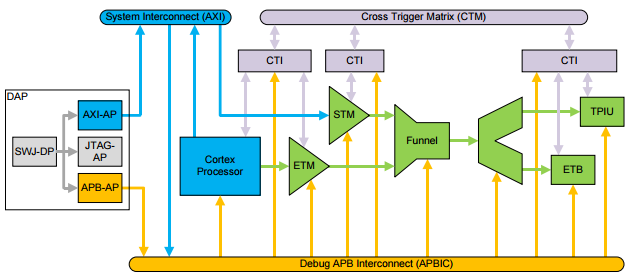
\includegraphics[width=\textwidth]{./Figures/coresight.png}
    \caption{Diagrama del módulo \emph{CoreSight}\protect\footnotemark.}
	\label{fig:coresight}
\end{figure}
\footnotetext{Imagen tomada del artículo \emph{How to debug: CoreSight basis} \citep{WEBSITE:coresight}.}

\section{Servidores y sondas de depuración}
\label{sec:depuracion}

Una sesión de depuración sirve para observar y modificar el estado de ejecución de un programa.
Esto se logra al leer y modificar los valores en registros del procesador y periféricos.
Además, se necesita de un sistema de disparos por eventos y supervisión de recursos.
Finalmente, la sesión debe detener la ejecución del núcleo de ser necesario.
En la figura \ref{fig:debug} se puede observar un esquema simplificado de una sesión de depuración.

\begin{figure}[htbp]
	\centering
	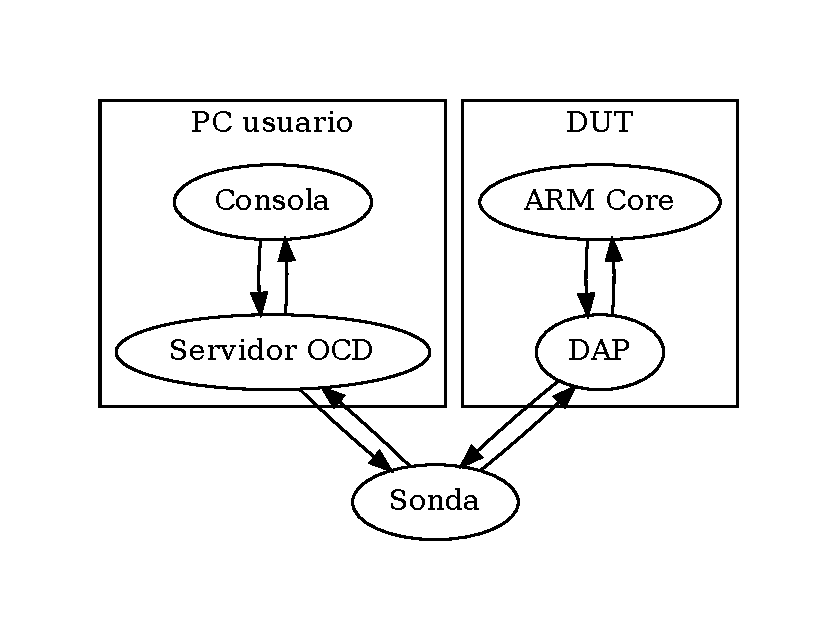
\includegraphics[width=.8\textwidth]{./Figures/debug.pdf}
    \caption{Conexión de una sesión de depuración.}
	\label{fig:debug}
\end{figure}

Un servidor \emph{On-chip debugger (OCD)} tiene la misión de abstraer la conexión de la sonda de depuración.
Además, facilita el manejo del ciclo de vida de la sesión y permite usar un \emph{software} como \emph{GNU Project debugger (GDB)}.
Finalmente, es la base de una pila de tecnologías que permite el uso de herramientas como \emph{GNU Emacs (Emacs)} \citep{BOOK:gdb}.
En la tabla \ref{tab:servidores} se puede observar un resumen de los servidores evaluados en el trabajo.

\begin{table}[h]
	\centering
	\caption[Servidores de depuración]{Comparativa entre servidores de depuración.}
	\begin{tabular}{l c c c}    
		\toprule
        \textbf{Servidor} & \textbf{API} & \textbf{Acceso}   & \textbf{Licencia}\\
		\midrule
        OpenOCD           & tcl                         & Registros y SDRAM & MIT\\        	
        PyOCD             & Python 3                    & Registros y SDRAM & Apache-2.0\\
		\bottomrule
		\hline
	\end{tabular}
	\label{tab:servidores}
\end{table}

El servidor OCD utilizado en este trabajo es PyOCD.
La principal característica que lo diferencia es el uso de Python 3 como lenguaje de \emph{scripting}.
Además, provee un servidor GDB, permite la programación de memoria \emph{flash} y ofrece una interfaz por consola de comandos \citep{WEBSITE:pyocd}.
Finalmente, los datos mas relevantes son:

\newpage

\begin{itemize}
    \item Requerimientos:
        \begin{itemize}
            \item Python 3.6.0 o superior.
            \item Una versión reciente de libusb.
            \item macOS, GNU Linux, Windows 7 o FreeBSD.
        \end{itemize}
    \item Sondas de depuración soportadas:
        \begin{itemize}
            \item Atmel EDBG/nEDBG.
            \item Atmel-ICE.
            \item Cypress KitProg3 o MiniProg4.
            \item DAPLink.
            \item Keil ULINKplus.
            \item NXP LPC-LinkII
            \item NXP MCU-Link
            \item PE Micro Cyclone y Multilink.
            \item Raspberry Pi Picoprobe.
            \item SEGGER J-Link.
            \item STLinkV2 y SRLinkV3.
        \end{itemize}
\end{itemize}




Las sondas de depuración tienen el objetivo de conectar el \emph{Debug Access Port} con el puerto del ordenador del usuario.
Adaptan los niveles de tensión y los protocolos involucrados.
Luego, permiten realizar una sesión de depuración, programar el dispositivo o verificar el estado de los componentes en la placa.
En la figura \ref{fig:sonda} se puede ver la sonda provista por el cliente.

\begin{figure}[htbp]
	\centering
	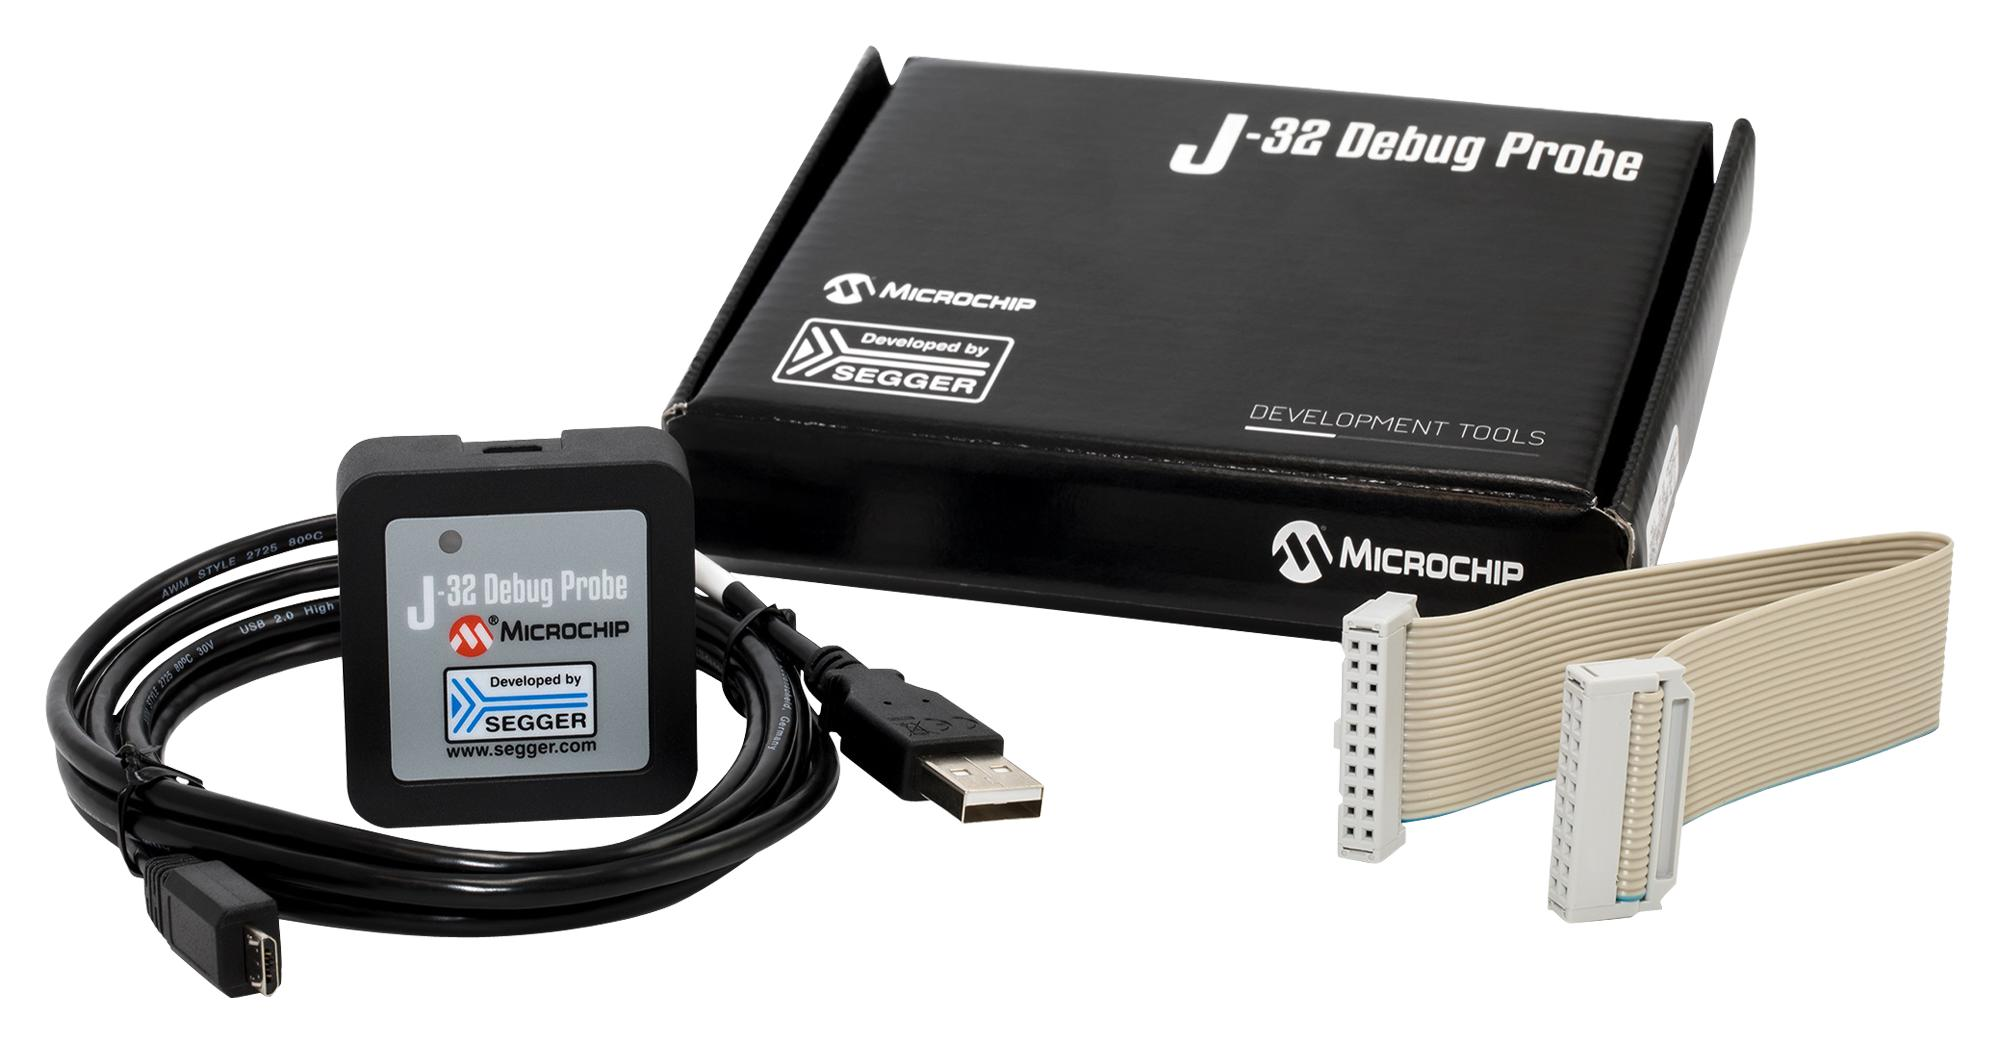
\includegraphics[width=.8\textwidth]{./Figures/segger.jpg}
    \caption{Sonda de depuración \emph{Segger J-32}\protect\footnotemark.}
	\label{fig:sonda}
\end{figure}
\footnotetext{Imagen tomada de \url{https://www.digikey.com/}}

\section{Periféricos de interés}
\label{sec:perifericos}

El dispositivo bajo prueba ofrece una variedad de periféricos para el desarrollo de aplicaciones.
Sin embargo, el cliente manifestó interés solo en los que se nombran a continuación:
\begin{itemize}
    \item CAN: este periférico permite al microcontrolador ser el dispositivo principal en una \emph{Controller Area Network}. La red es de grado industrial y fue diseñada para gestionar una red de sensores en un ambiente automotriz.
    \item PIO: es el puerto de entradas y salidas digitales de propósito general. En el caso del dispositivo bajo prueba, el periférico permite usar circuitos anti rebote, \emph{pull-up} y \emph{pull-down} internos. 
    \item SPI: el periférico permite realizar una conexión del tipo \emph{Serial Peripheral Interface}. Esta conexión es sincrónica y solo apta para distancias cortas.
    \item UART: es un periférico que permite conectarse a puertos y controlar dispositivos serie.
    \item Watchdog: el periférico sirve para detectar un error de ejecución y reiniciar el microprocesador.
\end{itemize}

En la tabla \ref{tab:perifericosresumen} se resume la funcionalidad de cada uno de ellos.

\begin{table}[h]
	\centering
	\caption[Resumen de periféricos]{Resumen de periféricos.}
	\begin{tabular}{l c c}    
		\toprule
        \textbf{Periférico} & \textbf{Funcionalidad}\\
		\midrule
		CAN                 & Bus de comunicación de grado industrial\\        	
		PIO                 & Entradas y salidas digitales\\
		SPI                 & Interfaz de comunicación sincrónica\\
		UART                & Puerto para dispositivos serie\\
		Watchdog            & Detección de errores y reinicio del integrado\\
		\bottomrule
		\hline
	\end{tabular}
	\label{tab:perifericosresumen}
\end{table}

\newpage

\section{Entornos de desarrollo}
\label{sec:entornos}

Para escribir el código que corre en el dispositivo bajo prueba se utilizó un entorno integrado de desarrollo (IDE).
Este IDE es MPLAB y fue provisto por el fabricante del integrado.
MPLAB está compuesto por una colección de programas que trabajan como un único sistema.
Entre ellos se encuentran:

\begin{itemize}
    \item Compilador para lenguaje C.
    \item Biblioteca CMSIS de ARM.
    \item Biblioteca HARMONY 3 de Microchip.
    \item Herramienta gráfica para la planificación de terminales.
    \item Herramienta gráfica para la configuración de periféricos.
    \item Herramienta gráfica para la configuración de reloj.
    \item Cliente GDB para sesiones de depuración.
\end{itemize}

Para realizar el código del inyector por consola de comandos se utilizó el lenguaje de programación Python 3.
Es un lenguaje interpretado que permite escribir código portable.
Además, el intérprete tiene la capacidad de crear ambientes virtuales.
Un ambiente virtual es un espacio de trabajo donde las dependencias instaladas quedan encapsuladas.
De esta manera, se puede simular el despliegue en un ambiente de producción.
Finalmente, junto al intérprete se utilizó un gestor de paquetes llamado PIP.
Esto facilitó la instalación automática del sistema.

Para escribir el código en Python 3, el \emph{firmware} en C y esta memoria en \LaTeX, se utilizó el editor de texto Neovim.
Este programa está basado en el editor Vi de los sistemas Unix.
Su funcionamiento es modal, esto significa que el editor funciona en los siguientes modos:

\begin{itemize}
    \item Modo normal:
        \begin{itemize}
            \item Navegar el documento.
            \item Ejecutar comandos de consola con la posibilidad de volcar el \emph{standard output} en el documento.
            \item Ejecutar \emph{scripts} de Neovim que permiten, por ejemplo, ordenar alfabéticamente una lista.
            \item Ejecutar búsquedas y reemplazos con comandos \emph{sed}.
            \item Grabar y ejecutar macros.
        \end{itemize}
    \item Modo inserción: permite escribir en el documento.
    \item Modo visual: permite seleccionar bloques del documento para aplicar comandos.
    \item Modo terminal: es un \emph{buffer} que emula una terminal Unix.
\end{itemize}

Neovim tiene la capacidad de conectarse a un servidor de análisis sintáctico de un lenguaje en particular.
Esto lo logra a través del \emph{Language Server Protocol (LSP)}.
El protocolo permite que un demonio realice el análisis de la sintaxis del código y envíe al editor información sobre errores y advertencias.
De esta manera se separa al editor del análisis sintáctico del lenguaje.
Además, Neovim tiene incorporado los diccionarios de la mayoría de los idiomas. Con solo ejecutar \texttt{:set spelllang=es} y \texttt{:set spell}, el editor resalta las palabras que no estén escritas en correcto castellano.

El último elemento del flujo de trabajo es el multiplexor de terminal Tmux.
Este programa permite dividir la terminal, crear \emph{buffers} y crear o conectarse a sesiones locales y remotas.
Esto posibilita partir una terminal y trabajar en simultáneo en dos o más ordenadores.
Finalmente, se trabajó de forma integrada con un ambiente de laboratorio remoto y sistemas de desarrollo locales.
En la figura \ref{fig:nvim} se puede ver un ejemplo del flujo de trabajo.

\begin{figure}[htbp]
	\centering
	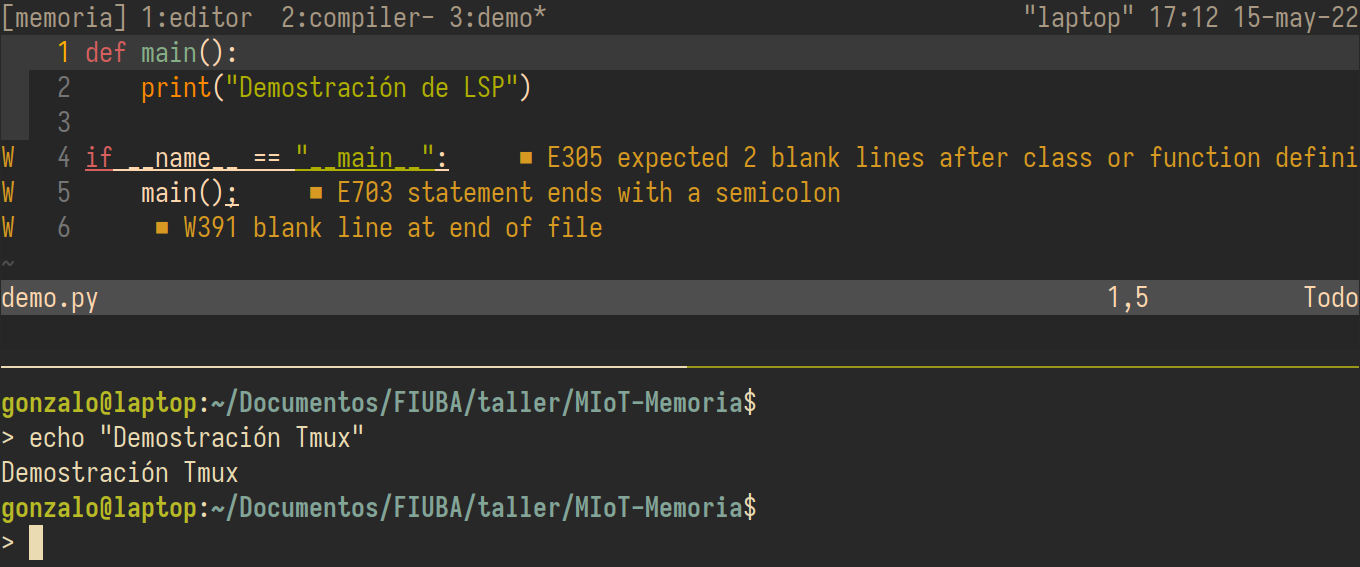
\includegraphics[width=\textwidth]{./Figures/nvimtmux.png}
    \caption{Ejemplo del flujo de trabajo Tmux-Neovim.}
	\label{fig:nvim}
\end{figure}

\newpage

\section{Requerimientos del cliente}
\label{sec:emphuerimientos}

Se realizaron una serie de reuniones con el cliente y se pudo definir los requerimientos del trabajo.
A continuación se enumeran los principales:

\begin{enumerate}
	\item Referentes al inyector por consola de comandos:
		\begin{enumerate}
			\item Generará de una interfaz de usuario.
			\item Permitirá configurar el ensayo a realizar.
			\item Observará la salida del dispositivo bajo prueba.
            \item Inyectará \emph{soft-errors} en el dispositivo bajo prueba.
			\item Persistirá las operaciones, entradas y salidas.
			\item Generará informes del ensayo realizado.
		\end{enumerate}
	\item Referentes al proceso del dispositivo bajo prueba:
		\begin{enumerate}
			\item Verificará el estado de los periféricos del dispositivo bajo prueba.
			\item Detectará si el dispositivo bajo prueba perdió su secuencia.
			\item Generará reportes de estado de periféricos y secuencia.
			\item Permitirá que el inyector por consola de comandos configure el alcance de la secuencia.
			\item Permitirá que el inyector por consola de comandos maneje el flujo de su secuencia.
		\end{enumerate}
\end{enumerate}

El cliente definió algunas restricciones para el desarrollo del sistema.
Estas se enumeran a continuación:

\begin{itemize}
	\item Utilización de un repositorio con control de versiones \emph{Gitlab}.
	\item Documentación del código con \emph{Doxygen}.
	\item Utilización exclusiva del lenguaje de programación \emph{Python 3}.
\end{itemize}

 
	\chapter{Diseño e implementación}
\label{Chapter3}

\definecolor{mygreen}{rgb}{0,0.6,0}
\definecolor{mygray}{rgb}{0.5,0.5,0.5}
\definecolor{mymauve}{rgb}{0.58,0,0.82}

\lstset{ %
  backgroundcolor=\color{white},   % choose the background color; you must add \usepackage{color} or \usepackage{xcolor}
  basicstyle=\footnotesize,        % the size of the fonts that are used for the code
  breakatwhitespace=false,         % sets if automatic breaks should only happen at whitespace
  breaklines=true,                 % sets automatic line breaking
  captionpos=b,                    % sets the caption-position to bottom
  commentstyle=\color{mygreen},    % comment style
  deletekeywords={...},            % if you want to delete keywords from the given language
  %escapeinside={\%*}{*)},          % if you want to add LaTeX within your code
  %extendedchars=true,              % lets you use non-ASCII characters; for 8-bits encodings only, does not work with UTF-8
  %frame=single,	                % adds a frame around the code
  keepspaces=true,                 % keeps spaces in text, useful for keeping indentation of code (possibly needs columns=flexible)
  keywordstyle=\color{blue},       % keyword style
  language=[ANSI]C,                % the language of the code
  %otherkeywords={*,...},           % if you want to add more keywords to the set
  numbers=left,                    % where to put the line-numbers; possible values are (none, left, right)
  numbersep=5pt,                   % how far the line-numbers are from the code
  numberstyle=\tiny\color{mygray}, % the style that is used for the line-numbers
  rulecolor=\color{black},         % if not set, the frame-color may be changed on line-breaks within not-black text (e.g. comments (green here))
  showspaces=false,                % show spaces everywhere adding particular underscores; it overrides 'showstringspaces'
  showstringspaces=false,          % underline spaces within strings only
  showtabs=false,                  % show tabs within strings adding particular underscores
  stepnumber=1,                    % the step between two line-numbers. If it's 1, each line will be numbered
  stringstyle=\color{mymauve},     % string literal style
  tabsize=2,	                   % sets default tabsize to 2 spaces
  title=\lstname,                  % show the filename of files included with \lstinputlisting; also try caption instead of title
  morecomment=[s]{/*}{*/}
}

Este capítulo detalla la generación de contenido original del trabajo.
Se explica su diseño y producción.

\section{Autoevaluación del dispositivo bajo prueba}
\label{sec:autoevaluacion}

La construcción del \emph{firmware} de autoevaluación del dispositivo bajo prueba requirió superar las siguientes etapas:
\begin{itemize}
    \item Configuración de las señales de reloj.
    \item Selección y configuración de los periféricos.
    \item Selección y configuración de los terminales externos.
    \item Implementación de las estrategias de validación de periféricos.
    \item Integración de una secuencia de validación y reporte.
\end{itemize}

Para configurar las frecuencias de reloj se buscó obtener 150 MHz para suministrar al \emph{Master CAN Bus}.
Con esta condición satisfecha, se pudo configurar las frecuencias de reloj del resto de los periféricos.
En la figura \ref{fig:clock} se puede observar la utilización del \emph{Programmable Clock Controller} número cinco.

\begin{figure}[htbp]
	\centering
	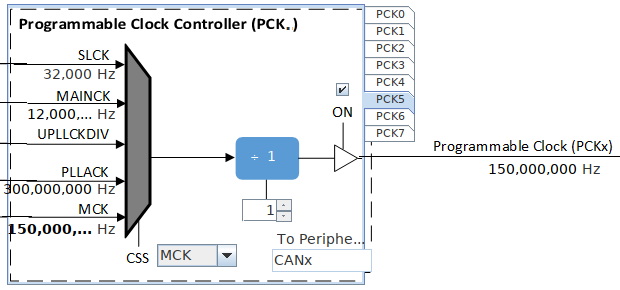
\includegraphics[width=\textwidth]{./Figures/Clock.png}
    \caption{Diagrama de configuración de las señales de reloj.}
	\label{fig:clock}
\end{figure}

El siguiente paso en la etapa de diseño fue la selección de las instancias de los periféricos del integrado.
Es posible que dos periféricos compartan parte del circuito interno o terminales del encapsulado.
Esta situación puede generar una disminución en las funcionalidades o una total incompatibilidad.
Finalmente, se seleccionaron instancias completamente disjuntas.

Luego de seleccionar las instancias de los periféricos, se configuraron para realizar un \emph{loopback}.
La configuración se realizó de la siguiente manera:

\begin{itemize}
    \item \emph{CAN}: se utilizó el \emph{MCAN1} con una configuración de \emph{loopback} interna, como se puede ver en la figura \ref{fig:canloopback}.
    \item \emph{PIO}: se configuraron dos terminales del dispositivo bajo prueba.
        El primero como salida sin \emph{latch} y el segundo como entrada sin circuito anti rebote.
    \item \emph{SPI}: la configuración elegida fue por defecto ya que el \emph{loopback} se logró conectando \emph{TX} y \emph{RX} con un cable.
    \item \emph{UART}: se configuró el periférico con una velocidad de 9600 baudios, 8 bits de datos y sin bits de paridad.
    \item \emph{Watchdog}: el disparo se configuró con un contador en 4095 cuentas.
        Este valor se estimó entre dos y cinco ejecuciones del \emph{loop} principal.
\end{itemize}

\begin{figure}[htbp]
	\centering
	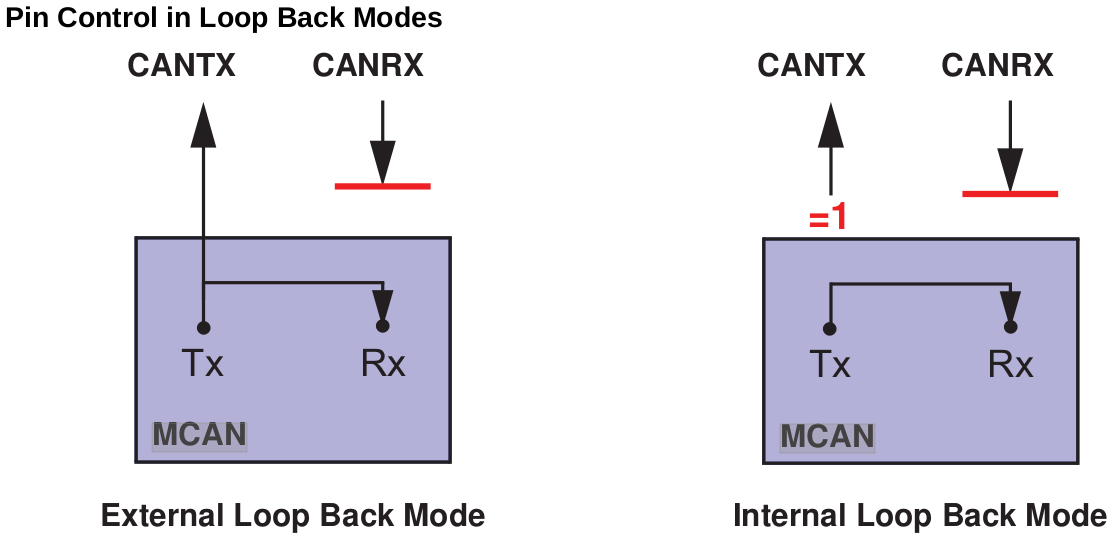
\includegraphics[width=0.8\textwidth]{./Figures/canloopback.png}
    \caption{Diagrama de \emph{loopback} del periférico \emph{CAN}\protect\footnotemark.}
	\label{fig:canloopback}
\end{figure}

\footnotetext{Imagen tomada de la hoja de datos del dispositivo bajo prueba \citep{ARTICLE:dutdatasheet}.}

Como se puede ver en la figura \ref{fig:labo}, se priorizaron los \emph{loopbacks} físicos externos.
Cuando esta estrategia no fue posible, se optó por internos provistos por el fabricante.
Finalmente, en los casos que las dos primeras opciones fueron imposibles, se utilizó una estrategia de \emph{software}.
En la tabla \ref{tab:perifericos} se puede ver un resumen de las estrategias aplicadas.

\begin{table}[h]
	\centering
	\caption[Estrategias de depuración]{Comparación entre estrategias de depuración}

	\begin{tabular}{l c c}    
		\toprule
        \textbf{Periférico} & \textbf{Validación}       & \textbf{Detección en un ciclo}\\
		\midrule
		CAN                 & Loopback interno          & Sí\\		
		PIO                 & Loopback externo          & No\\
		SPI                 & Loopback externo          & Sí\\
		UART                & Lógica en firmware        & No\\
		Watchdog            & Lógica en inyector        & No\\
		\bottomrule
		\hline
	\end{tabular}
	\label{tab:perifericos}
\end{table}

\begin{figure}[htbp]
	\centering
	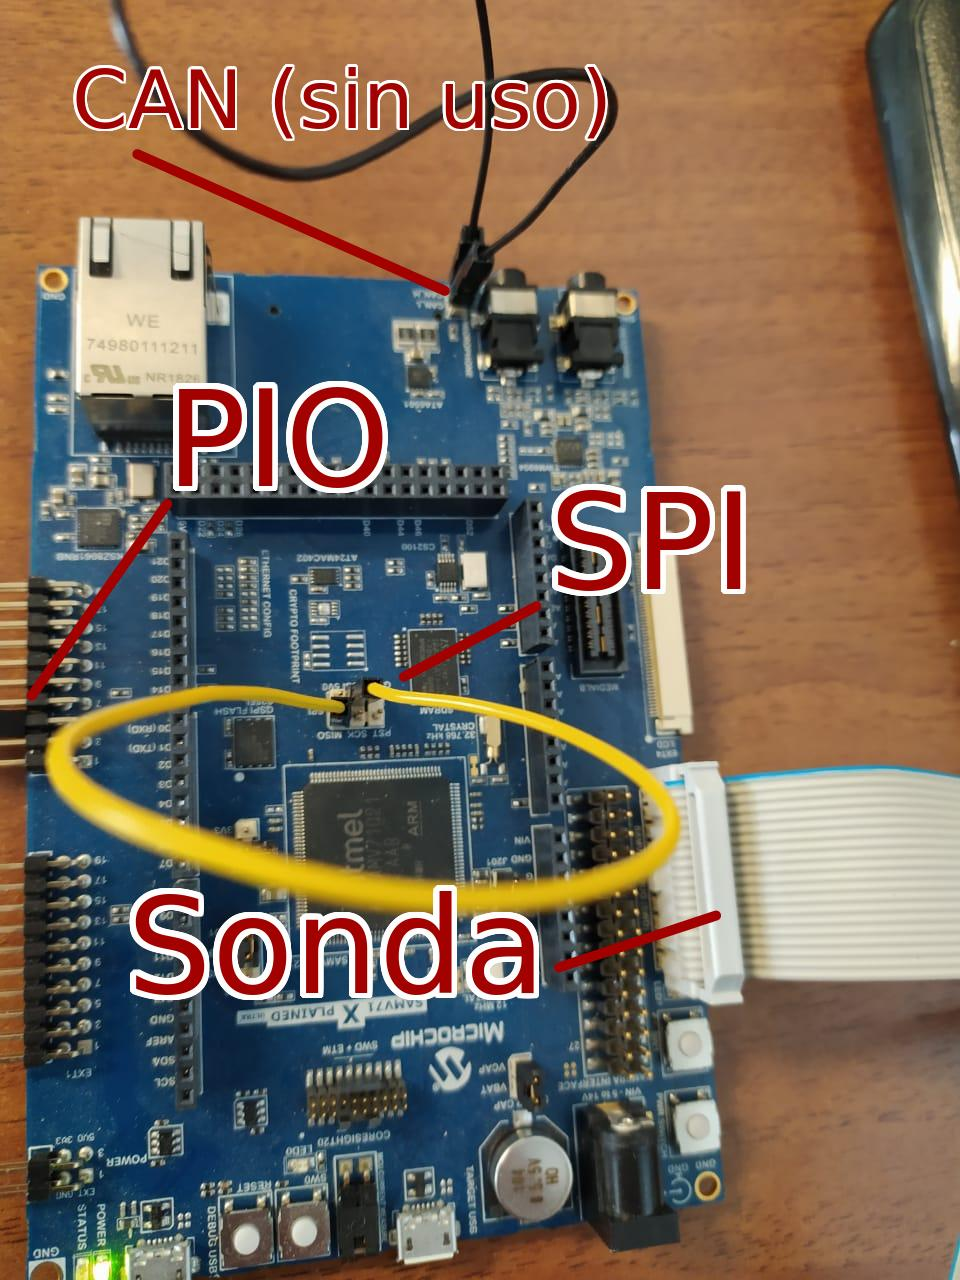
\includegraphics[width=\textwidth]{./Figures/labo.jpeg}
    \caption{Fotografía del dispositivo bajo prueba.}
	\label{fig:labo}
\end{figure}

\newpage

Una vez configurados los componentes de \emph{hardware} del dispositivo bajo prueba; se procedió a diseñar el \emph{firmware}.
Se comenzó con la estructura que define los reportes de estado del dispositivo bajo prueba.
Los reportes están formados por 2 bytes, el primero es el carácter ``F'' y marca el inicio del reporte mientras que el segundo byte lleva la información del estado de los periféricos.
En el código \ref{cod:structs} se puede ver la implementación del segundo byte del reporte.

\begin{lstlisting}[language=C,label=cod:structs,caption=Definición de la estructura de reportes.]  % Start your code-block

#define BIT 1

struct status_bitfield_t
{
    uint8_t CAN:BIT;
    uint8_t SPI:BIT;
    uint8_t PIO:BIT;
    uint8_t WATCHDOG:BIT;
}__attribute__((packed));

typedef union
{
    struct status_bitfield_t status_of;
    uint8_t packed;
}report_t;

\end{lstlisting}

En el código \ref{cod:loop} se puede observar la implementación del lazo principal.
Es importante notar que en la línea 10 se utilizó la \emph{union} para transformar el reporte en caracteres legibles para una persona.
En la figura \ref{fig:firmwareflow} se puede observar el flujo completo del programa.

\begin{lstlisting}[language=C,label=cod:loop,caption=Lazo principal del \emph{firmware} de autoevaluación.]  % Start your code-block

while ( true )
{
    SYS_Tasks ( );
    report.status_of.CAN = validate_CAN();
    report.status_of.PIO = validate_PIO();
    report.status_of.SPI = validate_SPI();
    report.status_of.WATCHDOG = NORMAL;
    
    buffer[FRAME_START] = 'F';
    buffer[FLAGS_INDEX] = report.packed + 'A';
    USART1_Write(&buffer[0], FRAME_SIZE);
    
    WDT_Clear();
}

\end{lstlisting}

\begin{figure}[htbp]
	\centering
	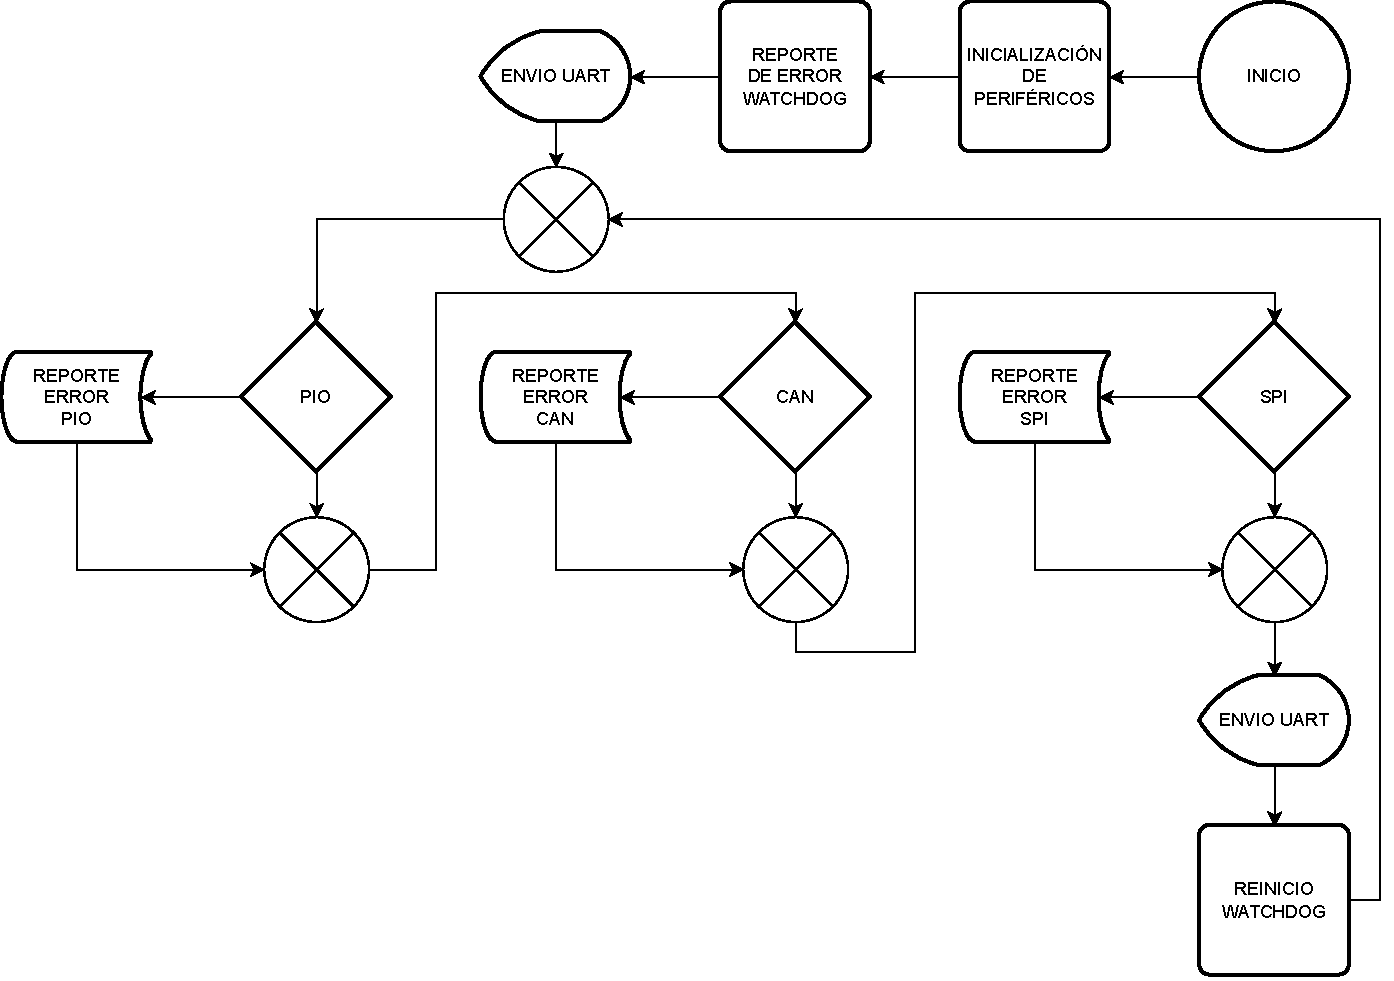
\includegraphics[width=\textwidth]{./Figures/firmwareflow.pdf}
    \caption{Flujo del \emph{firmware} de autoevaluación.}
	\label{fig:firmwareflow}
\end{figure}

\newpage

\section{Interfaz de programación de aplicaciones}
\label{sec:api}

% técnica RAII
% conexión como recurso
La interfaz de programación de aplicaciones tiene la función de abstraer al inyector de errores del servidor \emph{OCD}.
Esto se logró con los siguientes paradigmas y patrones de diseño:

\begin{itemize}
    \item Programación orientada a objetos \emph{(OOP)}: este paradigma de diseño se basa en agrupar en una unidad lógica las funcionalidades y estados que tengan un alto grado de acoplamiento.
        Esto significa que la funciones que tienen efectos colaterales junto a los datos mutados se encapsulan dentro de una construcción denominada objeto.
        Entonces, el principal objetivo de un objeto es contener dentro suyo los efectos colaterales.
        Además, el lenguaje de programación \emph{Python 3} permite, a través de una \emph{class}, modelar un tipo de dato para instanciar a un objeto.
        Finalmente, este patrón se utilizó para contener las funciones de lectura y escritura de registros y memorias.
    \item \emph{Resource Acquisition Is Initialization (RAII)}: este patrón de diseño consiste en modelar el ciclo de vida de un recurso con la implementación de un objeto.
        Un recurso es todo aquello que requiera mantenimiento luego de su uso, como por ejemplo: liberar memoria, cerrar una conexión o unir dos hilos de un programa.
        Esto se logra al adquirir un recurso cuando se invoca el constructor de una \emph{class}, por ejemplo, la conexión con la sonda de depuración se realiza durante la instanciación de un objeto llamado conexión.
        Luego, cuando se desea cerrar la conexión se invoca al destructor del objeto.
        Dentro de esta función se encuentra el código para cerrar de forma ordenada la conexión con la sonda y el dispositivo bajo prueba.
        Finalmente, este patrón de diseño hace que el programa maneje de forma robusta los recursos ya que está garantizada la ejecución de los destructores.
\end{itemize}

En el código \ref{cod:halted} se puede observar un ejemplo de \emph{RAII} donde se maneja como recurso la detención del núcleo del dispositivo bajo prueba.
Esto permite que frente a una excepción del proceso que esté utilizando la interfaz de programación de aplicaciones, el núcleo pueda continuar operando.
Finalmente, se posibilita recuperar el proceso sin tener que reiniciar el dispositivo bajo prueba.

\begin{lstlisting}[language=Python,label=cod:halted,caption=Ejemplo de \emph{Resource Acquisition Is Initialization (RAII)}.]  % Start your code-block

class Halted():
    def __init__(self, target):
        self.target = target

    def __enter__(self):
        self.target.halt()

    def __exit__(self, exc_type, exc_val, traceback):
        self.target.resume()

\end{lstlisting}

Los patrones de diseño utilizados permiten escribir funciones expresivas y robustas.
Como se puede ver en el código \ref{cod:haltedexample}, es fácil comprender lo que sucede.
En la línea 2 se detiene el núcleo y en la línea 3 se lee una posición de memoria.
Luego, en la línea 4 el núcleo reanuda su funcionamiento y finalmente, se retorna el valor leído.

\newpage

\begin{lstlisting}[language=Python,label=cod:haltedexample,caption=Ejemplo de uso de \emph{RAII}.]  % Start your code-block

def readMemory(self, addr: int):
    with Halted(self.target):
        val = self.target.read_memory(addr)
    return val

\end{lstlisting}

En la tabla \ref{tab:funcionalidades} se puede observar un resumen de las funcionalidades y sus estrategias de abstracción.

\begin{table}[h]
	\centering
	\caption[Funcionalidades abstraidas]{Funcionalidades abstraídas}

	\begin{tabular}{l c c}    
		\toprule
        \textbf{Funcionalidad}     & \textbf{Patrón de diseño} & \textbf{Acceso}\\
		\midrule
		Conexión al integrado      & RAII                      & Público\\		
		Detener el núcleo          & RAII                      & Privado\\
		Registros CORE: read/write & OOP                       & Público\\
		Memoria SDRAM: read/write  & OOP                       & Público\\
		\bottomrule
		\hline
	\end{tabular}
	\label{tab:funcionalidades}
\end{table}

Finalmente, se logró abstraer el ciclo de vida de la sesión de depuración que se muestra en la figura \ref{fig:debugsession}.

\begin{figure}[htbp]
	\centering
	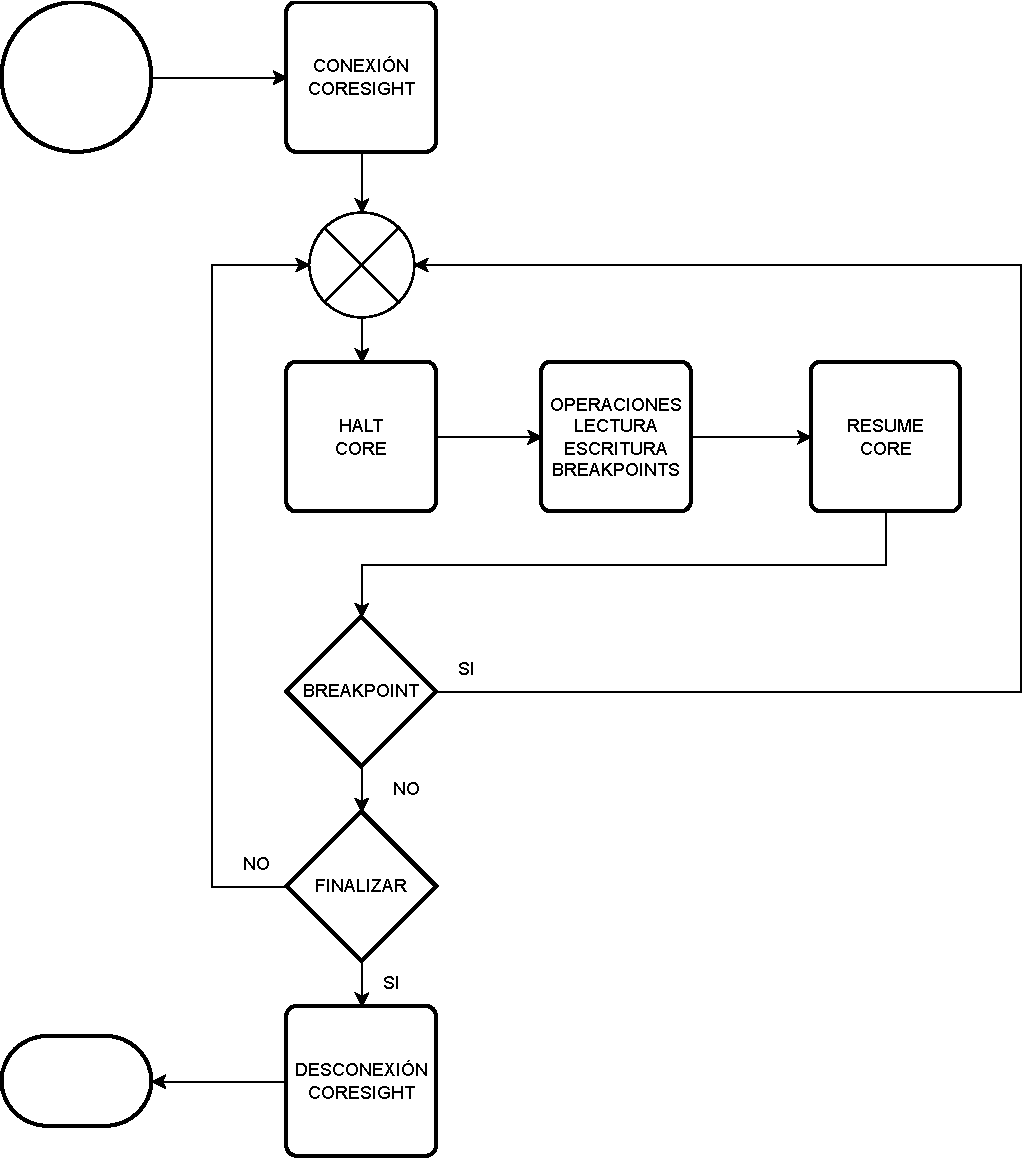
\includegraphics[width=0.9\textwidth]{./Figures/debugsession.pdf}
    \caption{Flujo de una sesión de depuración.}
	\label{fig:debugsession}
\end{figure}

\section{Sistema de inyección de \emph{soft-errors}}
\label{sec:sise}

Una vez lograda la interfaz de programación de aplicaciones explicada en la sección \ref{sec:api}, se pudo construir el inyector por consola de comandos que se muestra en la figura \ref{fig:siseblocks}.
Para lograr que el usuario utilice el programa se creó un sistema de archivo de configuración y un cliente de terminal en texto plano.
El archivo de configuración se genera en formato \emph{YAML} y se encarga de:

\begin{itemize}
    \item Definir si el controlador de ensayos debe recoger los reportes del dispositivo bajo prueba.
    \item Configurar el puerto serie del ordenador.
    \item Definir la simulación:
        \begin{itemize}
            \item El tipo de distribución para usar en el planificador de ensayos.
            \item La tasa de inyección de errores.
            \item La duración del tiempo de exposición en un registro o posición de memoria.
            \item La secuencia de exposición de los registros.
        \end{itemize}
\end{itemize}

% Configuración

En el código \ref{cod:yaml} se puede observar un archivo de configuración.
En particular, la configuración que el sistema ofrece como ejemplo al usuario.
Es importante notar que no se hace referencia a la sesión de depuración.
Finalmente, el ensayo se expresa en términos de parámetros de radiación.

Para facilitar la tarea del usuario, una vez instalado el sistema no es necesario trabajar en una carpeta en particular.
El inyector se puede invocar desde cualquier sitio donde el intérprete de Python 3 tenga permisos de ejecución.
El operador puede entonces crear una carpeta del ensayo.
Luego, crear un archivo de configuración y lanzar desde allí mismo la secuencia de inyecciones.
Finalmente, el sistema genera el reporte correspondiente en esa ruta.

\begin{lstlisting}[language=Python,label=cod:yaml,caption=Ejemplo de configuración de ensayo.]  % Start your code-block

# Perfil determina el tipo de ensayo a realizar
# 'simulador' solo genera inyecciones mientras
# que 'evaluador' recoge y procesa los
# reportes del DUT.
Perfil: 'simulador'

# Interfaz define el puerto serie donde se
# conecto el DUT.
Interfaz:
  puerto: '/dev/ttyACM0'
  baudios: 9600

# Simulacion define la forma de inyectar errores
Simulacion:
  distribucion: 'Poisson'
  tasa: 0.5
  duracion: 5
  registros: 'secuencial'

\end{lstlisting}

% Consola

La interfaz por consola se logró al utilizar el \emph{standar input} y el \emph{standar output} del proceso padre.
En el caso de una sesión iniciada por un humano, el emulador de terminal del sistema.
En una primera iteración de la consola se realizó una interfaz ASCII con la biblioteca \emph{curses}.
Sin embargo, el cliente prefirió una interfaz por texto plano para facilitar el \emph{parsing} de un sistema de integración continua.
En particular, el módulo de \emph{CI/CD} de \emph{Gitlab}.

El usuario invoca el programa al ejecutar el comando \texttt{sise}.
Luego la consola responde con la leyenda \texttt{Ingrese el archivo de configuración > }.
Se escribe la ruta y nombre del archivo a utilizar y el sistema lanza el ensayo.
El reporte generado se persiste en la carpeta donde se inició el programa.

% Planificador de ensayos

Con la información suministrada por el archivo de configuración y la consola, se puede iniciar el planificador de ensayos.
Este módulo tiene la función de generar una variable aleatoria que genera tiempos entre inyecciones de errores.
La variable aleatoria se construye con los datos de distribución y tasa de error.
El proceso aleatorio se repite hasta que la sumatoria de los tiempos generados sea igual o mayor al tiempo deseado del ensayo.
Luego, se asigna cada tiempo a un registro del núcleo en particular.
Esta asignación se realiza según la configuración del usuario.
Finalmente, se entrega la planificación al controlador de ensayos.

% Controlador de ensayos

El controlador de ensayos es un hilo del programa que tiene la misión de ejecutar una planificación de ensayos.
Su ejecución se basa en la interfaz de abstracción de aplicaciones explicada en la sección \ref{sec:api}.
Luego, tiene la responsabilidad de observar el tiempo de ejecución del dispositivo bajo prueba.
Cuando el momento es adecuado, el controlador invoca una función de \emph{bit flip}.
El bit a invertir se determina en el momento de inyección con una variable aleatoria uniforme.
Finalmente, cuando el controlador consume la totalidad de la planificación, envía una señal para solicitar el \emph{join} con el hilo principal del programa.

% Generador de reportes

El generador de reportes es un hilo que escucha el puerto serie del ordenador.
Mientras dura el ensayo, almacena todos los mensajes entrantes y los acumula junto a un \emph{timestamp}.
De la misma manera, persiste las inyecciones realizadas como tuplas.
Estas tuplas tienen todos los datos relevantes de la inyección junto a un \emph{timestamp}.
Cuando el ensayo finaliza, recibe una señal desde el hilo principal del programa que le ordena hacer un \emph{join}.
Luego, el generador de reportes deja de escuchar el puerto serie y al controlador de ensayos.
Seguidamente, se procede a construir un reporte en formato de tabla de \emph{MS Excel} y \emph{CSV}.
Para lograrlo, se genera una relación de causalidad entre errores inyectados y respuestas del dispositivo bajo prueba.
Finalmente, se generan los archivos en la carpeta donde el comando \texttt{sise} fue lanzado.

% Funcionamiento concurrente

La mayor dificultad del inyector fue el manejo concurrente de los hilos del controlador de ensayo y el generador de reportes.
En particular, porque ambos hilos comparten el uso del puerto serie.
Esta situación genera una condición de carrera que se tuvo que manejar.
Luego, se decidió evitar candados y semáforos al explotar la topología de \emph{bus} en árbol del protocolo \emph{USB}.
De esta manera, la conexión con la UART y el DAP se trató como si estuviesen conectados en puertos físicos diferentes.
Esta decisión de diseño tiene la ventaja de no incrementar el error de las mediciones de tiempo.
Un error en la medición generaría relaciones de causalidad incorrectas y por lo tanto los informes no serían confiables.
Sin embargo, se introdujo un punto de falla al depender de la capacidad de la sonda de depuración y su gestión de su árbol de dispositivos.
Finalmente, en la figura \ref{fig:concurrencia} se puede observar un diagrama con los hilos del programa.

\begin{figure}[htbp]
	\centering
	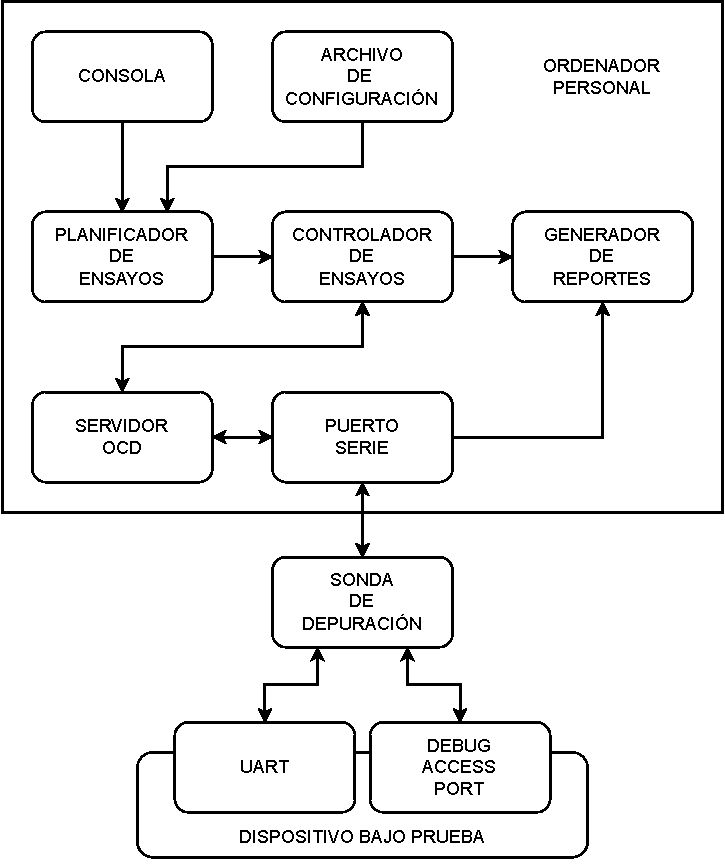
\includegraphics[width=\textwidth]{./Figures/siseblocks.pdf}
    \caption{Diagrama en bloques del sistema de inyección de soft-errors.}
	\label{fig:siseblocks}
\end{figure}

\begin{figure}[htbp]
	\centering
	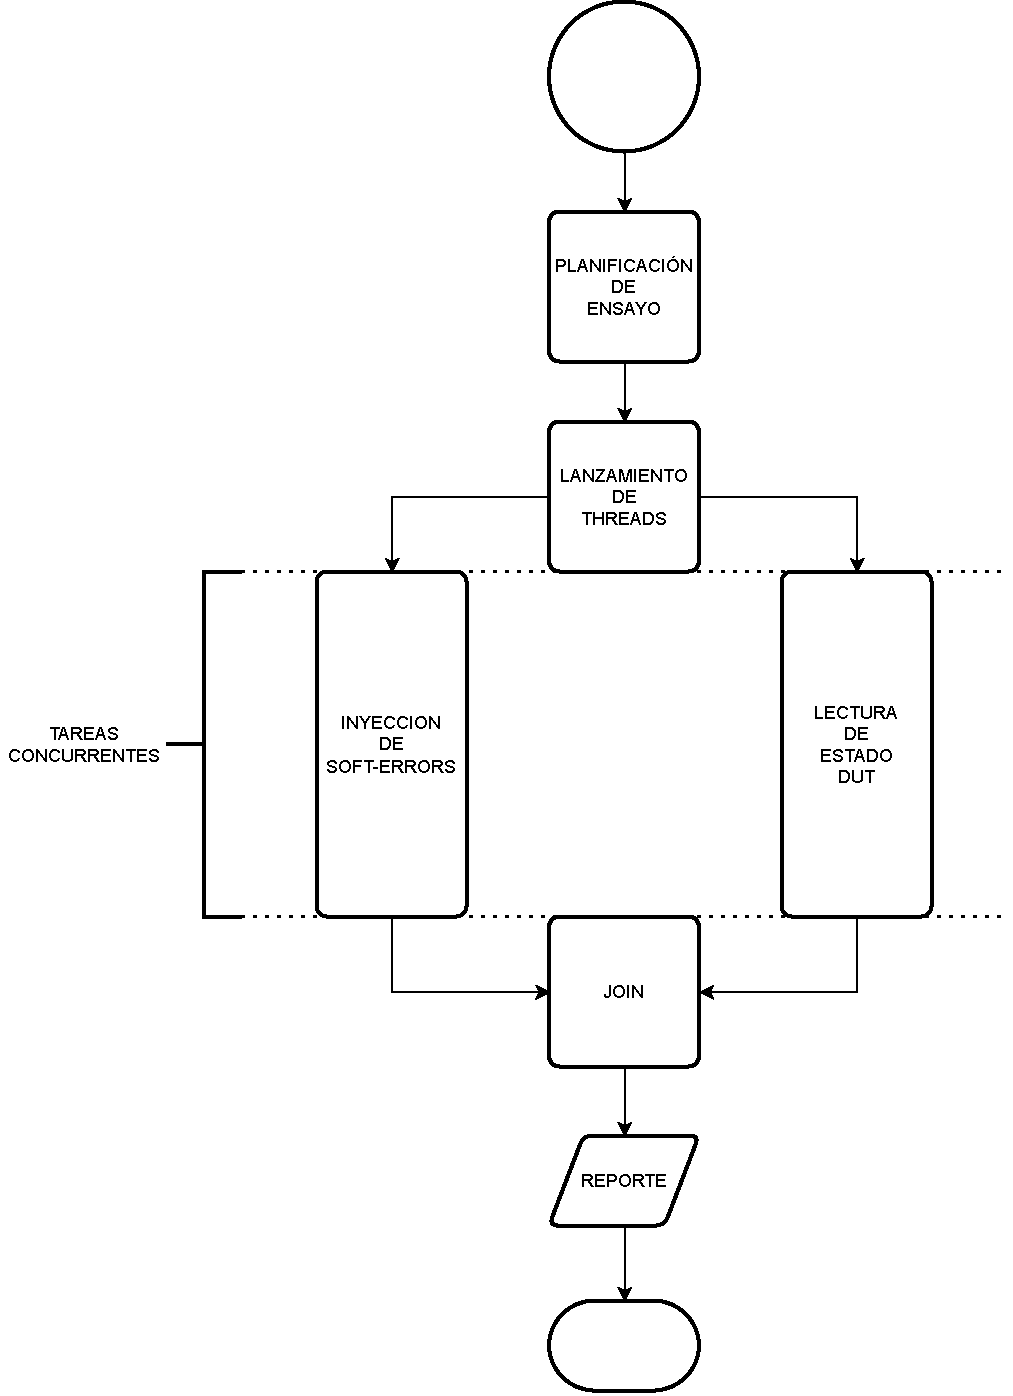
\includegraphics[width=\textwidth]{./Figures/concurrencia.pdf}
    \caption{Flujo de tareas concurrentes.}
	\label{fig:concurrencia}
\end{figure}

\section{Biblioteca para el desarrollo de ensayos}
\label{fig:biblioteca}

Para que el usuario pueda realizar sus propios ensayos, se creó una biblioteca que le provee la funcionalidad necesaria.
Esta biblioteca se divide en dos partes:

\begin{itemize}
    \item Funcionalidades del núcleo.
    \item Funcionalidades de la memoria.
\end{itemize}

Para facilitar la interacción con el núcleo se implementó una lista con los nombres de los registros.
De esta manera, se facilita el uso de las funciones.
En el código \ref{cod:corereg} se puede observar la colección que se le ofrece al diseñador.

\begin{lstlisting}[language=Python,label=cod:corereg,caption=Lista de registros accesibles por el usuario.]  % Start your code-block

CORE_REGISTERS = [
    'lr', 'pc', 'sp', 'xpsr', 'r0', 'r1', 'r2', 'r3',
    'r4', 'r5', 'r6', 'r7', 'r8', 'r9', 'r10', 'r11', 'r12'
]

\end{lstlisting}

Las funcionalidades ofrecidas para manipular el núcleo del integrado se muestran en el código \ref{cod:coreapi}.
Los detalles son los siguientes:

\begin{itemize}
    \item En la línea 6 se muestra el uso de la función de lectura de registros.
        Se invoca a partir del objeto de conexión y su argumento es el nombre del registro a leer.
    \item En la línea 10 se puede observar el uso del método de escritura de registros.
        Necesita como argumento el nombre del registro y el valor a escribir.
        Luego, la función retorna una tupla con los valores previos y posteriores a la escritura.
    \item En la línea 15 se ve una llamada a la función de \emph{bit flip} del registro del núcleo.
        Se debe indicar el nombre del registro y la posición del bit a invertir.
        Finalmente, se retorna el valor previo y posterior al llamado del método.
\end{itemize}

\newpage

\begin{lstlisting}[language=Python,label=cod:coreapi,caption=Ejemplo de uso en registros del núcleo.]  % Start your code-block

import sise.library as sise

dut = sise.Connection()

# Lectura del registro del CORE
rreg = dut.readRegister('pc')
print("PC:", rreg)

# Escritura del registro del CORE
wreg = writeRegister('r0', 0xffffffff)
print("(old, new):", wreg)

# Bit-flip en registro del CORE
bit = 2
bfreg = bitFlipRegister('r1', bit)
print("(old, new):", bfreg)

del(dut)

\end{lstlisting}

Para interactuar con la memoria se dispone de las funciones demostradas en el código \ref{cod:menapi}.
Los métodos se detallan a continuación:
\begin{itemize}
    \item Línea 7: el método permite realizar una lectura del dato en una posición de memoria.
        El argumento es una dirección alineada de la memoria y el retorno es el valor de una palabra de 32 bits.
    \item Línea 12: esta función se utiliza para escribir una posición alineada de memoria.
        Se necesita pasarle una dirección y un valor a escribir.
        Finalmente, retorna una tupla con el dato previo y posterior a la ejecución del método.
    \item Línea 18: la subrutina posibilita hacer un \emph{bit flip} en una posición de memoria.
        El método toma como argumento una posición alineada de memoria y el bit a invertir.
        Luego de su ejecución, se retorna el valor previo y posterior a la inversión.
\end{itemize}

\begin{lstlisting}[language=Python,label=cod:menapi,caption=Ejemplo de uso en memoria.]  % Start your code-block

import sise.library as sise

dut = sise.Connection()

# Lectura de memoria
addr = 0x20400004
rmen = readMemory(addr)
print("men:", rmen)

# Escritura de memoria
addr = 0x20400008
wmen = writeMemory(addr, 0xfafafafa):
print("(old, new):", wmen)

# Bit-flip en memoria
addr = 0x20400000
bit = 0
bfmen = dut.bitFlipMemory(addr, bit)
print("(old, new):", bfmen)

del(dut)

\end{lstlisting}

	% Chapter Template

\chapter{Ensayos y resultados} % Main chapter title

\label{Chapter4} % Change X to a consecutive number; for referencing this chapter elsewhere, use \ref{ChapterX}

En este capítulo se describe la estrategia de pruebas adoptada para determinar que el sistema se comporta de forma esperada.

%----------------------------------------------------------------------------------------
%	SECTION 1
%----------------------------------------------------------------------------------------

\section{Laboratorio remoto}
\label{sec:lab}

Durante las primeras etapas del desarrollo no se disponía en Buenos Aires del dispositivo bajo prueba.
Por esta razón, se montó un laboratorio remoto en San Carlos de Bariloche.
Se dispuso una placa de evaluación \emph{SAM V71 Xplained Ultra} conectada a un ordenador dentro de la red de INVAP S.E.
La conexión entre la placa y el ordenador se logró a través de una sonda de depuración \emph{Segger J-32}.

Para poder acceder al laboratorio remoto que se muestra en la figura \ref{fig:remotelab} se necesitó:

\begin{itemize}
    \item Credenciales de acceso y conexión a la VPN de INVAP S.E.
    \item Crear un túnel SSH con el ordenador remoto.
\end{itemize}

El túnel SSH se generó con \emph{X11 forwarding} habilitado.
De esta manera, se pudo generar ventanas gráficas en el ambiente local.
Además, las operaciones de consola se integraron al ordenador personal con una sesión de Tmux.
Finalmente, se logró implementar una interfaz de control del laboratorio remoto con una apariencia idéntica al ambiente local.

\begin{figure}[htbp]
	\centering
	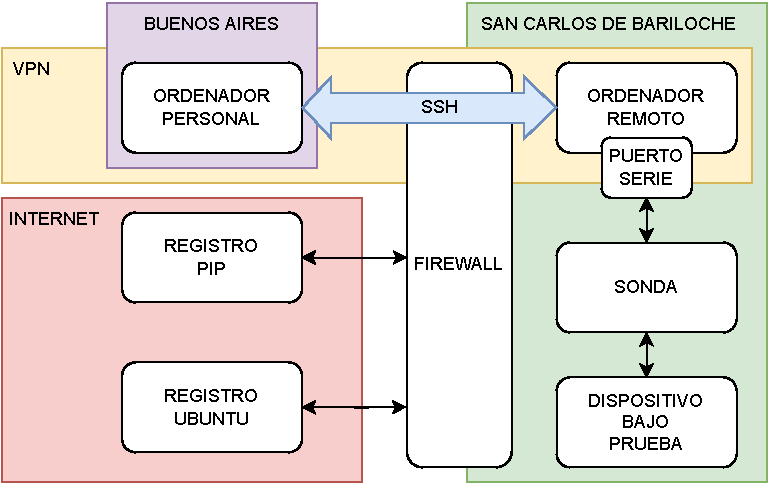
\includegraphics[width=\textwidth]{./Figures/vpn.pdf}
    \caption{Diagrama en bloques del laboratorio remoto.}
	\label{fig:remotelab}
\end{figure}

Para poder instalar las dependencias y los servidores OCD evaluados, se habilitaron los puertos necesarios que permitieron al ordenador remoto conectarse a los recursos en la Internet.
Sin embargo, algunos recursos debieron ser compilados en el \emph{host} y la transferencia de los \emph{tarballs} se realizó por medio de \emph{Secure Copy Files (scp)}.

Con el laboratorio remoto montado, se procedió a realizar las siguientes pruebas:
\begin{itemize}
    \item Pruebas de configuración de sondas de depuración y compatibilidad con servidores OCD.
    \item Pruebas de acceso al dispositivo bajo prueba.
\end{itemize}

Las pruebas referidas a la sonda de depuración arrojaron como resultado lo siguiente:

\begin{itemize}
    \item El modo de \emph{boot} de la sonda determina el nivel de acceso al dispositivo bajo prueba.
    \item Para lograr inyecciones de \emph{soft-errors} la sonda de depuración debe poder iniciar en modo \emph{CMSIS-DAP}.
    \item Si la sonda de depuración no se encuentra en modo \emph{CMSIS-DAP}, \emph{PyOCD} solo puede realizar escritura en la memoria \emph{flash}.
    \item Cambiar de modo una sonda de depuración requiere reiniciarla.
        Por lo tanto, no es factible realizar cambios de configuración luego de iniciado un ensayo.
\end{itemize}

Las pruebas referidas al acceso al dispositivo bajo prueba tuvieron los siguientes resultados:

\begin{itemize}
    \item Si no se dispone de un \emph{Device Family Pack (DFP)}, \emph{PyOCD} se conecta al dispositivo bajo prueba y lo identifica como \emph{Generic Cortex-M}.
    \item Bajo la identificación de \emph{Generic Cortex-M} se puede acceder a todos los registros de núcleo.
    \item Bajo la identificación de \emph{Generic Cortex-M} se puede acceder a la memoria \emph{SDRAM} y reconoce como error una posición desalineada.
    \item Bajo la identificación de \emph{Generic Cortex-M} se puede acceder a otras direcciones del integrado solo en modo lectura.
        Si se intenta ingresar en modo escritura no sucede ningún cambio pero el servidor OCD no responde con un error.
        Su respuesta es de operación exitosa, pero no se manifiestan cambios.
\end{itemize}

PyOCD posee un módulo de búsqueda y descarga de DFP, sin embargo, su funcionamiento no es confiable y genera una excepción durante su ejecución.
Se intentó verificar su funcionamiento en otras plataformas y se pudo observar que su desarrollo fue realizado en el lenguaje de programación \emph{Rust}.
Este módulo hizo imposible instalar el servidor OCD en una \emph{single board computer}.
Dado que, su compilador consume una cantidad de memoria que supera el \emph{hardware} disponible en placas como \emph{Raspberry Pi 4B}.
Se pudo verificar que este es el único módulo escrito en \emph{Rust}, pero no es posible desacoplarlo del servidor OCD.
Finalmente, PyOCD tiene una limitación de plataformas compatibles que podría ser sorteada con \emph{cross} compilación.

La única dificultad en el uso del laboratorio remoto se presentó en las pruebas de la sonda de depuración.
Muchas de las pruebas requirieron reiniciar la sonda y esto solo es posible al desconectar el cable \emph{USB}.
La operación debió ser realizada por el co-director de este trabajo.
En la tabla \ref{tab:funcionalidades}, se puede ver un resumen de las funcionalidades del laboratorio remoto.
Las funcionalidades con tres marcas tienen el mismo nivel de servicio que el laboratorio local, las de dos marcas tienen un nivel algo inferior y las que tienen solo una marca tienen un nivel de servicio bajo.

\begin{table}[h]
	\centering
	\caption[Resumen del laboratorio remoto]{Resumen del laboratorio remoto.}

	\begin{tabular}{l c}    
		\toprule
        \textbf{Funcionalidad}             & \textbf{Nivel de servicio} \\
		\midrule
		Carga de binarios en DUT           & ++  \\		
		Comunicación con registro PIP      & +++ \\
		Comunicación con registro Ubuntu   & +++ \\
		Comunicación con debug access port & +++ \\
		Comunicación con UART              & +   \\
		\bottomrule
		\hline
	\end{tabular}
	\label{tab:funcionalidades}
\end{table}

\section{Ensayos de inyector}
\label{sec:testinyector}

El inyector de \emph{soft-errors} se sometió a ensayos en los siguientes ambientes:

\begin{itemize}
    \item Laboratorio remoto.
    \item Laboratorio local.
    \item Dispositivo alternativo \emph{NUCLEO-F429ZI}.
        Este último ambiente se puede ver en la figura \ref{fig:alternativo} y se utilizó para probar si el inyector es genérico.
        En particular, porque utiliza una sonda de depuración distinta.
\end{itemize}

\begin{figure}[htbp]
	\centering
	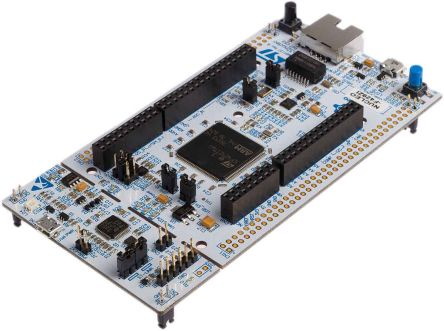
\includegraphics[width=0.8\textwidth]{./Figures/alternativo.jpg}
    \caption{Dispositivo alternativo \emph{NUCLEO-F429ZI}.}
	\label{fig:alternativo}
\end{figure}

Se generaron múltiples archivos de configuración para definir distintos casos de prueba.
Luego, se corrieron los ensayos en los tres ambientes y se compararon los resultados.
Además, se usó una variante adicional en el dispositivo alternativo.
Se probó el comportamiento del inyector sobre un blanco con \emph{mbedOS}.
Finalmente, en la tabla \ref{tab:resensayos} se puede observar un resumen de los resultados obtenidos.
En la tabla se marca con tres cruces los ensayos que arrojaron resultados sobresalientes, con dos cruces los ensayos que mostraron inconvenientes mínimos y con una cruz los ensayos con resultados insatisfactorios.

\begin{table}[h]
	\centering
	\caption[Resumen de ensayos]{Resumen de ensayos}

	\begin{tabular}{l c c c}    
		\toprule
        \textbf{Ensayo}                 & \textbf{Lab. local} & \textbf{Lab. remoto} & \textbf{DUT alterno} \\
		\midrule
		Escritura SDRAM                 & +++                 & +++                  & +++ \\
		Escritura registros CORE        & +++                 & +++                  & +++ \\
		Funcionalidades extras          & ++                  & ++                   & +++ \\
		Halt CORE                       & +++                 & +++                  & +++ \\
		Lectura SDRAM                   & +++                 & +++                  & +++ \\
		Lectura registros CORE          & +++                 & +++                  & +++ \\		
		Uso concurrente de puerto serie & +++                 & +                    & +++ \\
        Resume CORE                     & +++                 & +++                  & +++ \\
		\bottomrule
		\hline
	\end{tabular}
	\label{tab:resensayos}
\end{table}

El dispositivo alternativo arrojó los mejores resultados porque PyOCD tiene el \emph{Device Family Pack}.
Por otro lado, el laboratorio remoto tuvo malos resultados en las pruebas de concurrencia.
Esto fue así ya que se debía pedir ayuda al personal de INVAP S.E. cada vez que la sonda necesitaba ser reiniciada. 

\section{Validación con el cliente}
\label{sec:validacion}

La etapa final del proceso de pruebas fue una serie de demostraciones realizadas al cliente.
Luego de cada demostración se indicaban las correcciones a realizar.
Seguidamente, se mejoraba el código y se repetía la demostración.
Estos ciclos de iteraciones tenían una frecuencia de 15 días.
Finalmente, se llegó al cumplimiento total de los requerimientos como se puede ver en la tabla \ref{tab:validacion}

\begin{table}[h]
	\centering
	\caption[Resumen de la validación con el cliente]{Resumen de la validación con el cliente}

	\begin{tabular}{l c}    
		\toprule
        \textbf{Expectativas}     & \textbf{Cumplimiento} \\
		\midrule
		Acceso a memoria          & +++                   \\
		Acceso al CORE            & +++                   \\
		Biblioteca de ensayos     & +++                   \\		
		Capacidad de bit-flip     & +++                   \\
		Configuración del sistema & +++                   \\
		Distribución de errores   & +++                   \\
		Validación de periféricos & +++                   \\
        Generación de reportes    & +++                   \\
		\bottomrule
		\hline
	\end{tabular}
	\label{tab:validacion}
\end{table}

En la figura \ref{fig:demobitflip} se puede observar una demostración del acceso a memoria SDRAM.
Se puede ver que la terminal está dividida en las siguientes partes:

\begin{itemize}
    \item Sección izquierda: se hizo una demostración paso a paso.
        Primero, se importó la biblioteca dentro del espacio de trabajo.
        Luego, se conectó al dispositivo y se cargó una dirección de memoria y el bit a invertir.
        Seguidamente, se realizó una inversión y se mostró el valor previo y posterior al \emph{bit flip}.
        Finalmente, se cerró la conexión con el dispositivo alternativo.
    \item Sección derecha: se observa el mapa de memoria SDRAM del dispositivo alternativo.
        Se usó para mostrarle al cliente las direcciones de memoria ensayadas.
\end{itemize}

Este ensayo además de demostrar el acceso a memoria SDRAM también ejercita la capacidad de realizar \emph{bit flip}.
Finalmente, el cliente consideró que se habían cumplido todos los requisitos y que el trabajo se encontraba finalizado.

Los ensayos finales se volvieron a reproducir en presencia de un estudiante de la especialización en sistemas embebidos quién actualmente utiliza la herramienta en el marco de su proyecto final.

\begin{figure}[htbp]
	\centering
	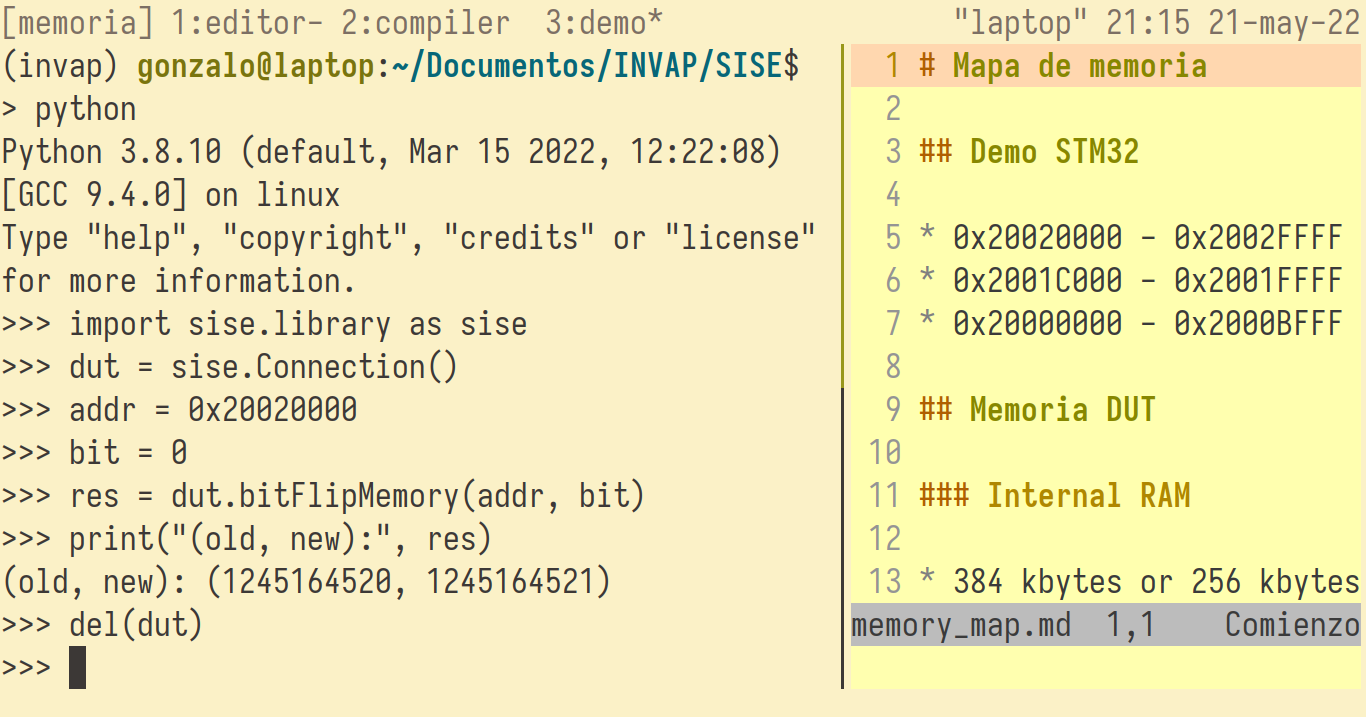
\includegraphics[width=\textwidth]{./Figures/demo_bitflip.png}
    \caption{Demostración de acceso a memoria.}
	\label{fig:demobitflip}
\end{figure}
 
	\chapter{Conclusiones}
\label{Chapter5}

Este capítulo explica de forma breve el cierre del trabajo realizado, sus logros y futuro.

\section{Resultados obtenidos}
\label{sec:5resultados}

El trabajo logró cumplir las expectativas y requerimientos del cliente.
En particular, los siguientes objetivos:

\begin{itemize}
    \item Creación de un sistema de inyección de \emph{soft-errors} que permita evaluar técnicas de mitigación de errores.
    \item Acceso a la memoria volátil del dispositivo bajo prueba.
    \item Biblioteca para el diseño de ensayos en lenguaje \emph{Python 3}.
\end{itemize}

La recepción de este trabajo fue muy positiva; ya que en la actualidad, INVAP S.E. se encuentra en proceso de integrar la herramienta en su ambiente de desarrollo de satélites.
Además, el sistema realizado se utiliza dentro del marco de un proyecto final en la Especialización en Sistemas Embebidos.

\section{Trabajo futuro}
\label{sec:5futuro}

La investigación realizada durante la producción del trabajo sugiere que es posible agregar las siguientes funcionalidades:

\begin{itemize}
    \item Conexión entre el código fuente del dispositivo bajo prueba y el inyector de \emph{soft-errors}.
    \item Creación de instrucciones específicas para la inyección de \emph{single event functional interrupt}.
\end{itemize}
 
\end{verbatim}

Los apéndices también deben escribirse en archivos .tex separados, que se deben ubicar dentro de la carpeta \emph{Appendices}. Los apéndices vienen comentados por defecto con el caracter \code{\%} y para incluirlos simplemente se debe eliminar dicho caracter.

Finalmente, se encuentra el código para incluir la bibliografía en el documento final.  Este código tampoco debe modificarse. La metodología para trabajar las referencias bibliográficas se desarrolla en la sección \ref{sec:biblio}.
%----------------------------------------------------------------------------------------

\section{Bibliografía}
\label{sec:biblio}

Las opciones de formato de la bibliografía se controlan a través del paquete de latex \option{biblatex} que se incluye en la memoria en el archivo memoria.tex.  Estas opciones determinan cómo se generan las citas bibliográficas en el cuerpo del documento y cómo se genera la bibliografía al final de la memoria.

En el preámbulo se puede encontrar el código que incluye el paquete biblatex, que no requiere ninguna modificación del usuario de la plantilla, y que contiene las siguientes opciones:

\begin{lstlisting}
\usepackage[backend=bibtex,
	natbib=true, 
	style=numeric, 
	sorting=none]
{biblatex}
\end{lstlisting}

En el archivo \file{reference.bib} se encuentran las referencias bibliográficas que se pueden citar en el documento.  Para incorporar una nueva cita al documento lo primero es agregarla en este archivo con todos los campos necesario.  Todas las entradas bibliográficas comienzan con $@$ y una palabra que define el formato de la entrada.  Para cada formato existen campos obligatorios que deben completarse. No importa el orden en que las entradas estén definidas en el archivo .bib.  Tampoco es importante el orden en que estén definidos los campos de una entrada bibliográfica. A continuación se muestran algunos ejemplos:

\begin{lstlisting}
@ARTICLE{ARTICLE:1,
    AUTHOR="John Doe",
    TITLE="Title",
    JOURNAL="Journal",
    YEAR="2017",
}
\end{lstlisting}


\begin{lstlisting}
@BOOK{BOOK:1,
    AUTHOR="John Doe",
    TITLE="The Book without Title",
    PUBLISHER="Dummy Publisher",
    YEAR="2100",
}
\end{lstlisting}


\begin{lstlisting}
@INBOOK{BOOK:2,
    AUTHOR="John Doe",
    TITLE="The Book without Title",
    PUBLISHER="Dummy Publisher",
    YEAR="2100",
    PAGES="100-200",
}
\end{lstlisting}


\begin{lstlisting}
@MISC{WEBSITE:1,
    HOWPUBLISHED = "\url{http://example.com}",
    AUTHOR = "Intel",
    TITLE = "Example Website",
    MONTH = "12",
    YEAR = "1988",
    URLDATE = {2012-11-26}
}
\end{lstlisting}

Se debe notar que los nombres \emph{ARTICLE:1}, \emph{BOOK:1}, \emph{BOOK:2} y \emph{WEBSITE:1} son nombres de fantasía que le sirve al autor del documento para identificar la entrada. En este sentido, se podrían reemplazar por cualquier otro nombre.  Tampoco es necesario poner : seguido de un número, en los ejemplos sólo se incluye como un posible estilo para identificar las entradas.

La entradas se citan en el documento con el comando: 

\begin{verbatim}
\citep{nombre_de_la_entrada}
\end{verbatim}

Y cuando se usan, se muestran así: \citep{ARTICLE:1}, \citep{BOOK:1}, \citep{BOOK:2}, \citep{WEBSITE:1}.  Notar cómo se conforma la sección Bibliografía al final del documento. 

\chapter{Introducción específica}

\label{Chapter2}

En este capítulo se detallan las tecnologías que forman parte del trabajo.
Son productos de terceros que se integran en las herramientas entregadas al cliente.

\section{Arquitectura del dispositivo bajo prueba}
\label{sec:dut}

El trabajo fue realizado para un tipo de microcontrolador específico.
Su diseño forma parte de la familia \emph{Cortex M7} de la empresa \emph{ARM}.
En la figura \ref{fig:cortexm} se puede observar un diagrama en bloques de la arquitectura.

El dispositivo bajo prueba es el microcontrolador \emph{SAM V71} diseñado por la empresa \emph{Atmel} y comercializado por \emph{Microchip}.
El integrado fue pensado para aplicaciones automotrices según el estándar \emph{ISO-TS-16949}.
Además, el circuito puede operar con un reloj de 300 MHz y almacenar un programa de 2048 kB.
Las estructuras de datos del programa pueden aprovechar la memoria cache dual de 16 kB \citep{ARTICLE:dutdatasheet}.
Las principales características del dispositivo bajo prueba son:

\begin{itemize}
    \item Núcleo:
        \begin{itemize}
            \item Unidad de punto flotante de precisión simple y doble.
            \item Unidad de protección de memoria con 16 zonas.
            \item Instrucciones para el procesamiento digital de señales.
        \end{itemize}
    \item Memorias:
        \begin{itemize}
            \item \emph{ROM} de 16 kB con rutinas de inicialización. Esto permite iniciar el sistema desde los periféricos \emph{UART0} y \emph{USB}.
            \item Controlador de memoria estática para el uso de memorias externas.
        \end{itemize}
    \item Sistema:
        \begin{itemize}
            \item Reloj de tiempo real con gestión de calendario gregoriano.
            \item Reinicio por alimentación, detección de caída de tensión y doble \emph{Watchdog}.
            \item Puerto dual de 24 canales para la gestión de acceso a memoria.
            \item Compensación por variaciones de reloj.
        \end{itemize}
\end{itemize}

\newpage

Este integrado fue sometido a una prueba por radiación donde se evaluaron SEE y la calificación de dosis total de ionización (TID).
El microcontrolador mantuvo su funcionamiento en todo el rango de temperatura de calificación militar.
Además, el dispositivo es inmune a \emph{Single Event Latch-up} con una tolerancia de 60,0 $MeV.cm^2/mg$.
Esta sensibilidad fue probada con una cámara de iones pesados.
En cuanto a la calificación de dosis total de ionización, el lote fue sometido a un ensayo de 30 krad(Si) y la prueba fue superada.
Finalmente, los ensayos suministrados por el fabricante permiten concluir que no es necesario realizar inyecciones de errores en la memoria \emph{flash} \citep{ARTICLE:dutrad}.

Al fabricante del dispositivo bajo prueba se le impone respetar el mapa de memoria y registros del núcleo.
Esto permitió construir un inyector de \emph{soft-errors} genérico.
Finalmente, la herramienta entregada funciona para cualquier integrado de la familia \emph{Cortex M}.

\begin{figure}[htbp]
	\centering
	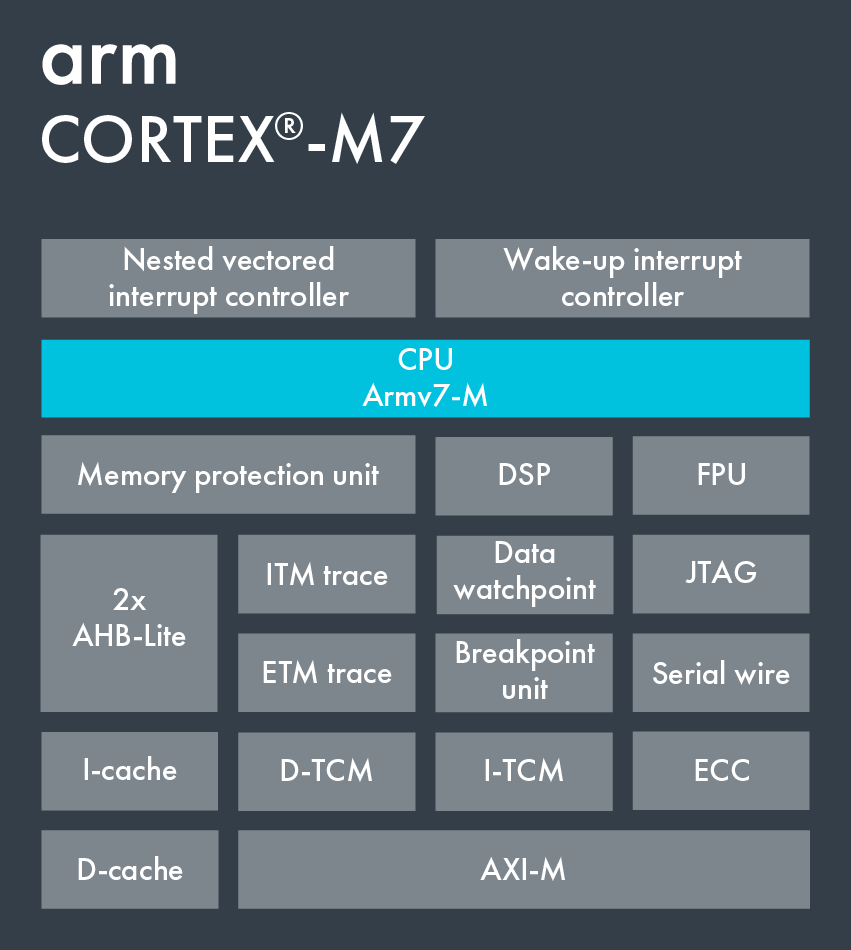
\includegraphics[width=.7\textwidth]{./Figures/Cortex-M7.png}
    \caption{Diagrama de la arquitectura \emph{Cortex M7}\protect\footnotemark.}
	\label{fig:cortexm}
\end{figure}

\footnotetext{Imagen tomada de la página oficial de \emph{ARM Developers}. \citep{WEBSITE:cortexm}}

La arquitectura tiene un módulo que permite programar y depurar el integrado.
Este módulo se denomina \emph{CoreSight} y es propio de los dispositivos \emph{ARM}.
En la figura \ref{fig:coresight} se muestra un diagrama en bloques del módulo.
Sus partes principales son:

\begin{itemize}
    \item \emph{Cross Triggering}: permite conectar y encaminar las señales que utilizan las sondas de depuración.
        En la figura \ref{fig:coresight} está representada en los bloques \emph{CTI}.
        Además, se unen a través del \emph{Cross Trigger Matrix (CTM)}.
    \item \emph{Debug Access Port (DAP)}: es el puerto físico para conectar la sonda de depuración. Es una implementación de la interfaz de depuración \emph{ARM}.
    \item \emph{Embedded Trace Macrocells}: permite extraer información y controlar el núcleo del dispositivo.
    \item \emph{Instrumentation Trace Units}: permite que una sonda de depuración se conecte con las \emph{Embedded Trace Macrocells}.
    \item \emph{ROM Tables}: sirven para que la sonda de depuración identifique al integrado.
    \item \emph{Self Hosted Debug}: son instrucciones específicas de depuración controladas por un procesador secundario.
    \item \emph{Trace Interconnect}: provee puentes para compartir señales de reloj, alimentación y otras señales comunes.
\end{itemize}

\begin{figure}[htbp]
	\centering
	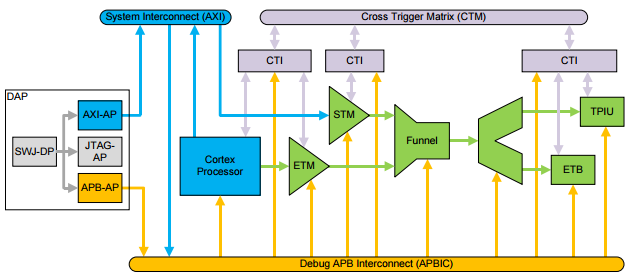
\includegraphics[width=\textwidth]{./Figures/coresight.png}
    \caption{Diagrama del módulo \emph{CoreSight}\protect\footnotemark.}
	\label{fig:coresight}
\end{figure}
\footnotetext{Imagen tomada del artículo \emph{How to debug: CoreSight basis} \citep{WEBSITE:coresight}.}

\section{Servidores y sondas de depuración}
\label{sec:depuracion}

Una sesión de depuración sirve para observar y modificar el estado de ejecución de un programa.
Esto se logra al leer y modificar los valores en registros del procesador y periféricos.
Además, se necesita de un sistema de disparos por eventos y supervisión de recursos.
Finalmente, la sesión debe detener la ejecución del núcleo de ser necesario.
En la figura \ref{fig:debug} se puede observar un esquema simplificado de una sesión de depuración.

\begin{figure}[htbp]
	\centering
	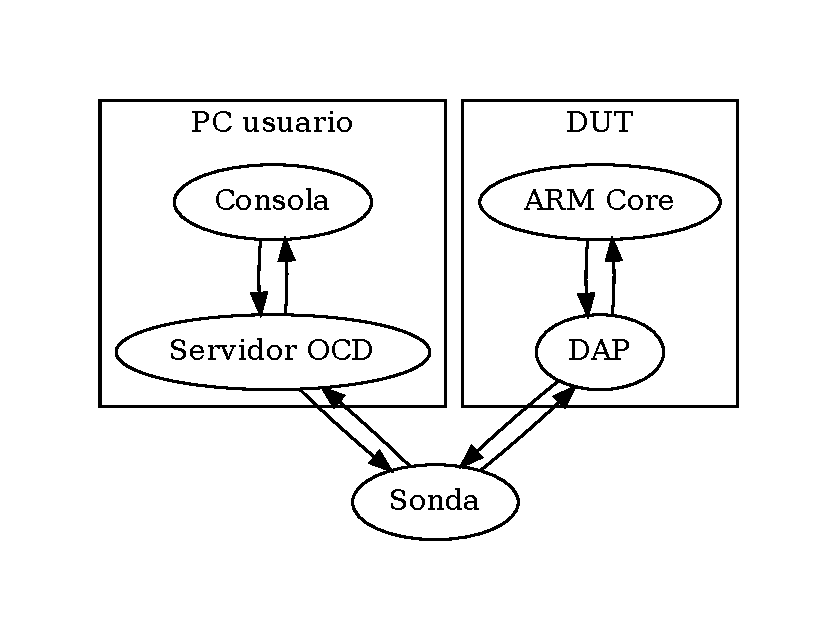
\includegraphics[width=.8\textwidth]{./Figures/debug.pdf}
    \caption{Conexión de una sesión de depuración.}
	\label{fig:debug}
\end{figure}

Un servidor \emph{On-chip debugger (OCD)} tiene la misión de abstraer la conexión de la sonda de depuración.
Además, facilita el manejo del ciclo de vida de la sesión y permite usar un \emph{software} como \emph{GNU Project debugger (GDB)}.
Finalmente, es la base de una pila de tecnologías que permite el uso de herramientas como \emph{GNU Emacs (Emacs)} \citep{BOOK:gdb}.
En la tabla \ref{tab:servidores} se puede observar un resumen de los servidores evaluados en el trabajo.

\begin{table}[h]
	\centering
	\caption[Servidores de depuración]{Comparativa entre servidores de depuración.}
	\begin{tabular}{l c c c}    
		\toprule
        \textbf{Servidor} & \textbf{API} & \textbf{Acceso}   & \textbf{Licencia}\\
		\midrule
        OpenOCD           & tcl                         & Registros y SDRAM & MIT\\        	
        PyOCD             & Python 3                    & Registros y SDRAM & Apache-2.0\\
		\bottomrule
		\hline
	\end{tabular}
	\label{tab:servidores}
\end{table}

El servidor OCD utilizado en este trabajo es PyOCD.
La principal característica que lo diferencia es el uso de Python 3 como lenguaje de \emph{scripting}.
Además, provee un servidor GDB, permite la programación de memoria \emph{flash} y ofrece una interfaz por consola de comandos \citep{WEBSITE:pyocd}.
Finalmente, los datos mas relevantes son:

\newpage

\begin{itemize}
    \item Requerimientos:
        \begin{itemize}
            \item Python 3.6.0 o superior.
            \item Una versión reciente de libusb.
            \item macOS, GNU Linux, Windows 7 o FreeBSD.
        \end{itemize}
    \item Sondas de depuración soportadas:
        \begin{itemize}
            \item Atmel EDBG/nEDBG.
            \item Atmel-ICE.
            \item Cypress KitProg3 o MiniProg4.
            \item DAPLink.
            \item Keil ULINKplus.
            \item NXP LPC-LinkII
            \item NXP MCU-Link
            \item PE Micro Cyclone y Multilink.
            \item Raspberry Pi Picoprobe.
            \item SEGGER J-Link.
            \item STLinkV2 y SRLinkV3.
        \end{itemize}
\end{itemize}




Las sondas de depuración tienen el objetivo de conectar el \emph{Debug Access Port} con el puerto del ordenador del usuario.
Adaptan los niveles de tensión y los protocolos involucrados.
Luego, permiten realizar una sesión de depuración, programar el dispositivo o verificar el estado de los componentes en la placa.
En la figura \ref{fig:sonda} se puede ver la sonda provista por el cliente.

\begin{figure}[htbp]
	\centering
	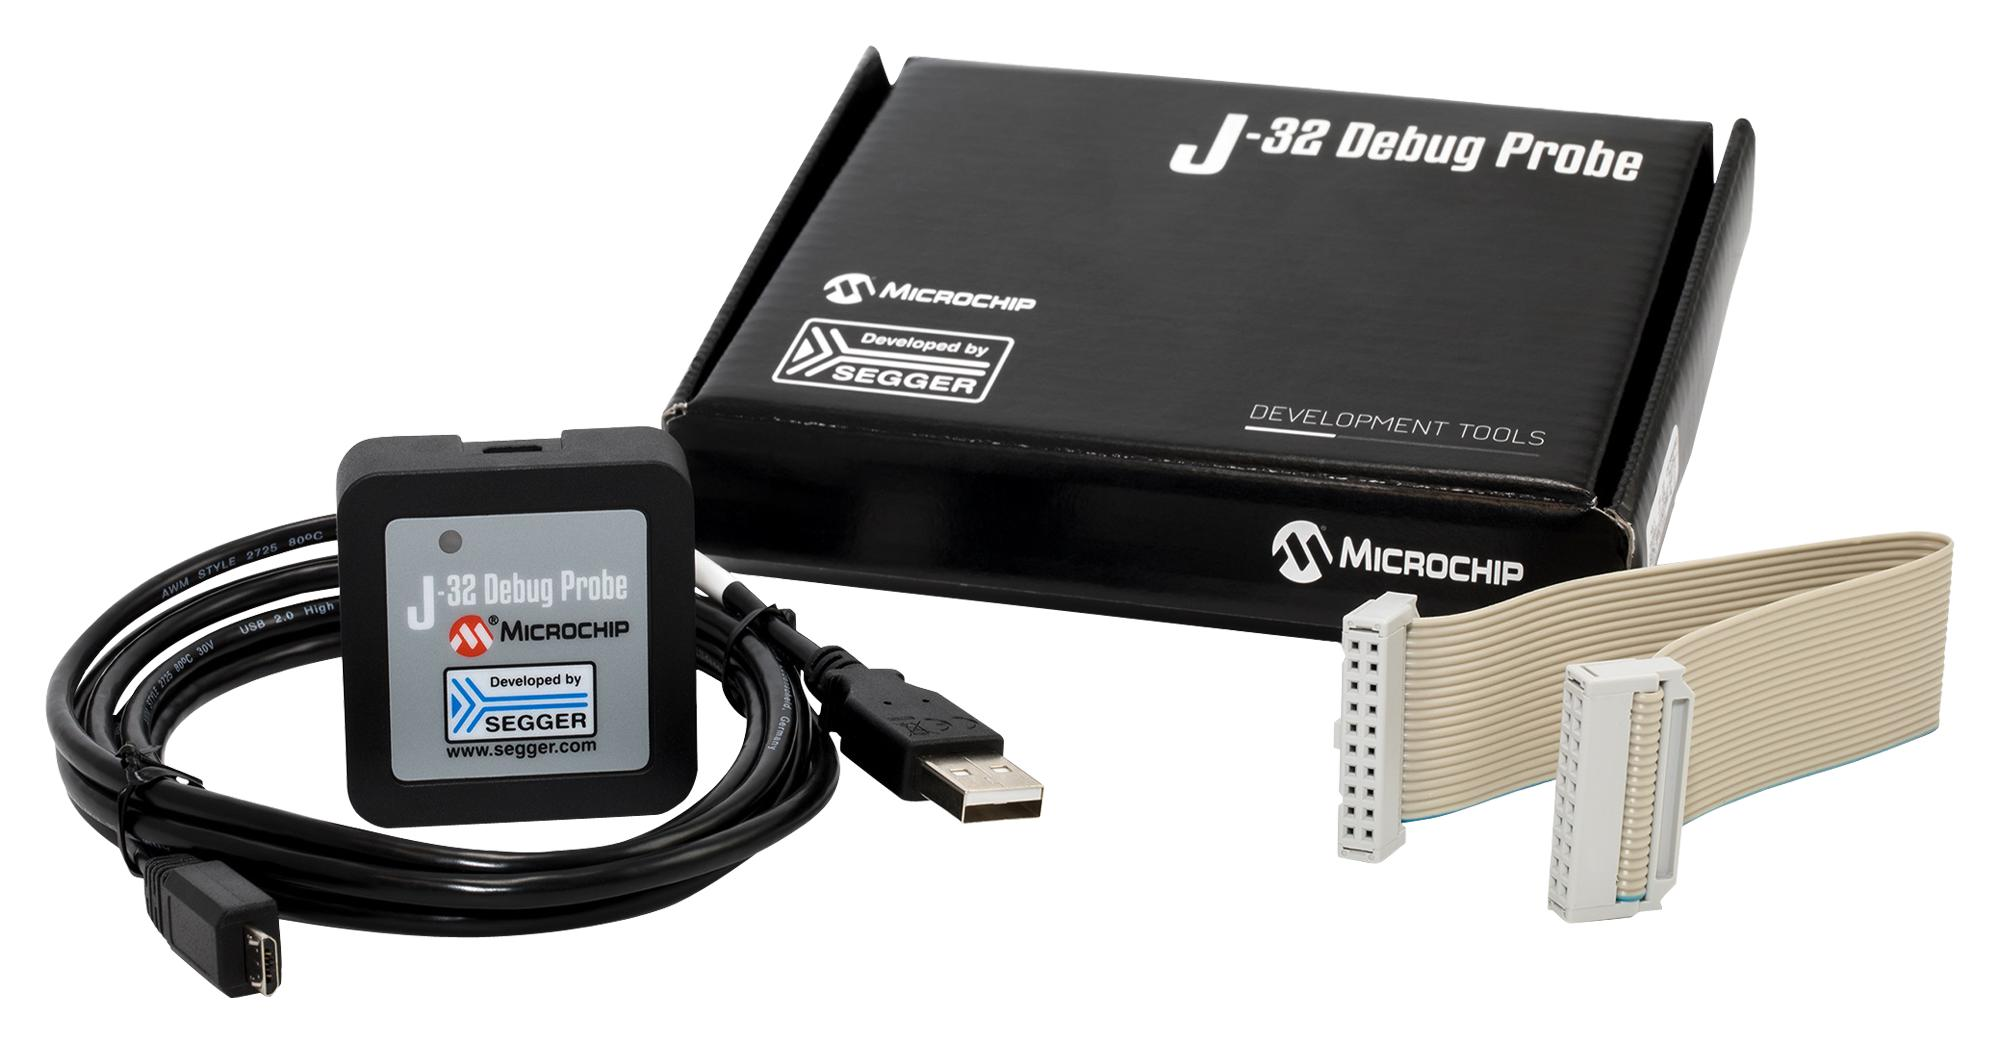
\includegraphics[width=.8\textwidth]{./Figures/segger.jpg}
    \caption{Sonda de depuración \emph{Segger J-32}\protect\footnotemark.}
	\label{fig:sonda}
\end{figure}
\footnotetext{Imagen tomada de \url{https://www.digikey.com/}}

\section{Periféricos de interés}
\label{sec:perifericos}

El dispositivo bajo prueba ofrece una variedad de periféricos para el desarrollo de aplicaciones.
Sin embargo, el cliente manifestó interés solo en los que se nombran a continuación:
\begin{itemize}
    \item CAN: este periférico permite al microcontrolador ser el dispositivo principal en una \emph{Controller Area Network}. La red es de grado industrial y fue diseñada para gestionar una red de sensores en un ambiente automotriz.
    \item PIO: es el puerto de entradas y salidas digitales de propósito general. En el caso del dispositivo bajo prueba, el periférico permite usar circuitos anti rebote, \emph{pull-up} y \emph{pull-down} internos. 
    \item SPI: el periférico permite realizar una conexión del tipo \emph{Serial Peripheral Interface}. Esta conexión es sincrónica y solo apta para distancias cortas.
    \item UART: es un periférico que permite conectarse a puertos y controlar dispositivos serie.
    \item Watchdog: el periférico sirve para detectar un error de ejecución y reiniciar el microprocesador.
\end{itemize}

En la tabla \ref{tab:perifericosresumen} se resume la funcionalidad de cada uno de ellos.

\begin{table}[h]
	\centering
	\caption[Resumen de periféricos]{Resumen de periféricos.}
	\begin{tabular}{l c c}    
		\toprule
        \textbf{Periférico} & \textbf{Funcionalidad}\\
		\midrule
		CAN                 & Bus de comunicación de grado industrial\\        	
		PIO                 & Entradas y salidas digitales\\
		SPI                 & Interfaz de comunicación sincrónica\\
		UART                & Puerto para dispositivos serie\\
		Watchdog            & Detección de errores y reinicio del integrado\\
		\bottomrule
		\hline
	\end{tabular}
	\label{tab:perifericosresumen}
\end{table}

\newpage

\section{Entornos de desarrollo}
\label{sec:entornos}

Para escribir el código que corre en el dispositivo bajo prueba se utilizó un entorno integrado de desarrollo (IDE).
Este IDE es MPLAB y fue provisto por el fabricante del integrado.
MPLAB está compuesto por una colección de programas que trabajan como un único sistema.
Entre ellos se encuentran:

\begin{itemize}
    \item Compilador para lenguaje C.
    \item Biblioteca CMSIS de ARM.
    \item Biblioteca HARMONY 3 de Microchip.
    \item Herramienta gráfica para la planificación de terminales.
    \item Herramienta gráfica para la configuración de periféricos.
    \item Herramienta gráfica para la configuración de reloj.
    \item Cliente GDB para sesiones de depuración.
\end{itemize}

Para realizar el código del inyector por consola de comandos se utilizó el lenguaje de programación Python 3.
Es un lenguaje interpretado que permite escribir código portable.
Además, el intérprete tiene la capacidad de crear ambientes virtuales.
Un ambiente virtual es un espacio de trabajo donde las dependencias instaladas quedan encapsuladas.
De esta manera, se puede simular el despliegue en un ambiente de producción.
Finalmente, junto al intérprete se utilizó un gestor de paquetes llamado PIP.
Esto facilitó la instalación automática del sistema.

Para escribir el código en Python 3, el \emph{firmware} en C y esta memoria en \LaTeX, se utilizó el editor de texto Neovim.
Este programa está basado en el editor Vi de los sistemas Unix.
Su funcionamiento es modal, esto significa que el editor funciona en los siguientes modos:

\begin{itemize}
    \item Modo normal:
        \begin{itemize}
            \item Navegar el documento.
            \item Ejecutar comandos de consola con la posibilidad de volcar el \emph{standard output} en el documento.
            \item Ejecutar \emph{scripts} de Neovim que permiten, por ejemplo, ordenar alfabéticamente una lista.
            \item Ejecutar búsquedas y reemplazos con comandos \emph{sed}.
            \item Grabar y ejecutar macros.
        \end{itemize}
    \item Modo inserción: permite escribir en el documento.
    \item Modo visual: permite seleccionar bloques del documento para aplicar comandos.
    \item Modo terminal: es un \emph{buffer} que emula una terminal Unix.
\end{itemize}

Neovim tiene la capacidad de conectarse a un servidor de análisis sintáctico de un lenguaje en particular.
Esto lo logra a través del \emph{Language Server Protocol (LSP)}.
El protocolo permite que un demonio realice el análisis de la sintaxis del código y envíe al editor información sobre errores y advertencias.
De esta manera se separa al editor del análisis sintáctico del lenguaje.
Además, Neovim tiene incorporado los diccionarios de la mayoría de los idiomas. Con solo ejecutar \texttt{:set spelllang=es} y \texttt{:set spell}, el editor resalta las palabras que no estén escritas en correcto castellano.

El último elemento del flujo de trabajo es el multiplexor de terminal Tmux.
Este programa permite dividir la terminal, crear \emph{buffers} y crear o conectarse a sesiones locales y remotas.
Esto posibilita partir una terminal y trabajar en simultáneo en dos o más ordenadores.
Finalmente, se trabajó de forma integrada con un ambiente de laboratorio remoto y sistemas de desarrollo locales.
En la figura \ref{fig:nvim} se puede ver un ejemplo del flujo de trabajo.

\begin{figure}[htbp]
	\centering
	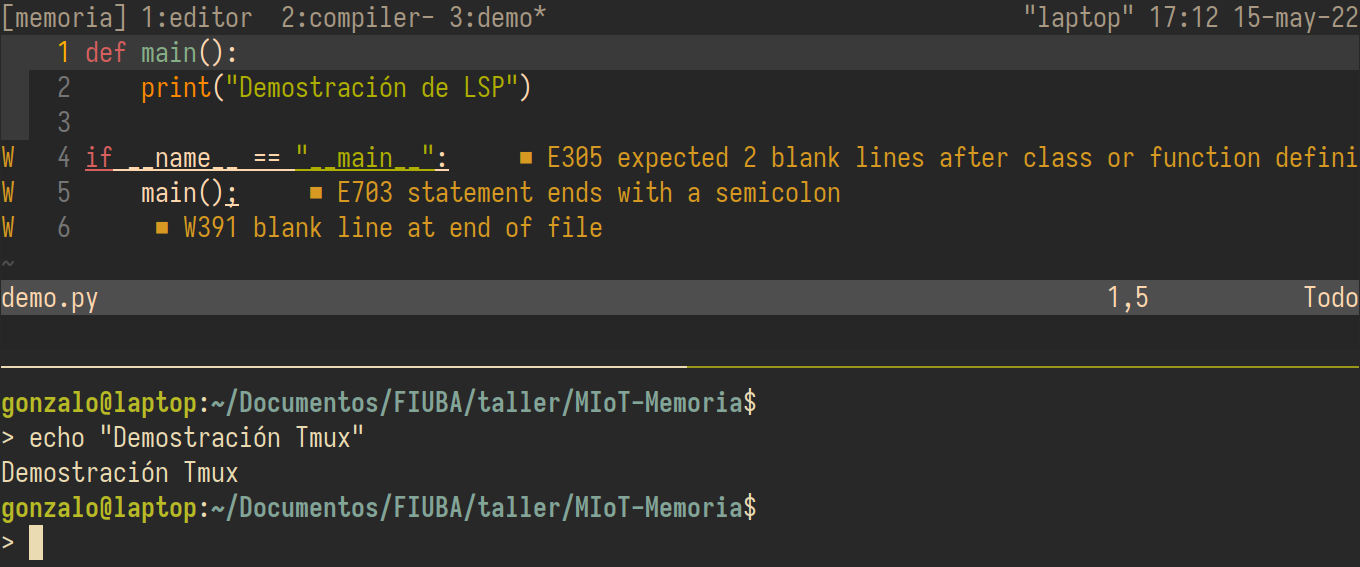
\includegraphics[width=\textwidth]{./Figures/nvimtmux.png}
    \caption{Ejemplo del flujo de trabajo Tmux-Neovim.}
	\label{fig:nvim}
\end{figure}

\newpage

\section{Requerimientos del cliente}
\label{sec:emphuerimientos}

Se realizaron una serie de reuniones con el cliente y se pudo definir los requerimientos del trabajo.
A continuación se enumeran los principales:

\begin{enumerate}
	\item Referentes al inyector por consola de comandos:
		\begin{enumerate}
			\item Generará de una interfaz de usuario.
			\item Permitirá configurar el ensayo a realizar.
			\item Observará la salida del dispositivo bajo prueba.
            \item Inyectará \emph{soft-errors} en el dispositivo bajo prueba.
			\item Persistirá las operaciones, entradas y salidas.
			\item Generará informes del ensayo realizado.
		\end{enumerate}
	\item Referentes al proceso del dispositivo bajo prueba:
		\begin{enumerate}
			\item Verificará el estado de los periféricos del dispositivo bajo prueba.
			\item Detectará si el dispositivo bajo prueba perdió su secuencia.
			\item Generará reportes de estado de periféricos y secuencia.
			\item Permitirá que el inyector por consola de comandos configure el alcance de la secuencia.
			\item Permitirá que el inyector por consola de comandos maneje el flujo de su secuencia.
		\end{enumerate}
\end{enumerate}

El cliente definió algunas restricciones para el desarrollo del sistema.
Estas se enumeran a continuación:

\begin{itemize}
	\item Utilización de un repositorio con control de versiones \emph{Gitlab}.
	\item Documentación del código con \emph{Doxygen}.
	\item Utilización exclusiva del lenguaje de programación \emph{Python 3}.
\end{itemize}

 
\chapter{Diseño e implementación}
\label{Chapter3}

\definecolor{mygreen}{rgb}{0,0.6,0}
\definecolor{mygray}{rgb}{0.5,0.5,0.5}
\definecolor{mymauve}{rgb}{0.58,0,0.82}

\lstset{ %
  backgroundcolor=\color{white},   % choose the background color; you must add \usepackage{color} or \usepackage{xcolor}
  basicstyle=\footnotesize,        % the size of the fonts that are used for the code
  breakatwhitespace=false,         % sets if automatic breaks should only happen at whitespace
  breaklines=true,                 % sets automatic line breaking
  captionpos=b,                    % sets the caption-position to bottom
  commentstyle=\color{mygreen},    % comment style
  deletekeywords={...},            % if you want to delete keywords from the given language
  %escapeinside={\%*}{*)},          % if you want to add LaTeX within your code
  %extendedchars=true,              % lets you use non-ASCII characters; for 8-bits encodings only, does not work with UTF-8
  %frame=single,	                % adds a frame around the code
  keepspaces=true,                 % keeps spaces in text, useful for keeping indentation of code (possibly needs columns=flexible)
  keywordstyle=\color{blue},       % keyword style
  language=[ANSI]C,                % the language of the code
  %otherkeywords={*,...},           % if you want to add more keywords to the set
  numbers=left,                    % where to put the line-numbers; possible values are (none, left, right)
  numbersep=5pt,                   % how far the line-numbers are from the code
  numberstyle=\tiny\color{mygray}, % the style that is used for the line-numbers
  rulecolor=\color{black},         % if not set, the frame-color may be changed on line-breaks within not-black text (e.g. comments (green here))
  showspaces=false,                % show spaces everywhere adding particular underscores; it overrides 'showstringspaces'
  showstringspaces=false,          % underline spaces within strings only
  showtabs=false,                  % show tabs within strings adding particular underscores
  stepnumber=1,                    % the step between two line-numbers. If it's 1, each line will be numbered
  stringstyle=\color{mymauve},     % string literal style
  tabsize=2,	                   % sets default tabsize to 2 spaces
  title=\lstname,                  % show the filename of files included with \lstinputlisting; also try caption instead of title
  morecomment=[s]{/*}{*/}
}

Este capítulo detalla la generación de contenido original del trabajo.
Se explica su diseño y producción.

\section{Autoevaluación del dispositivo bajo prueba}
\label{sec:autoevaluacion}

La construcción del \emph{firmware} de autoevaluación del dispositivo bajo prueba requirió superar las siguientes etapas:
\begin{itemize}
    \item Configuración de las señales de reloj.
    \item Selección y configuración de los periféricos.
    \item Selección y configuración de los terminales externos.
    \item Implementación de las estrategias de validación de periféricos.
    \item Integración de una secuencia de validación y reporte.
\end{itemize}

Para configurar las frecuencias de reloj se buscó obtener 150 MHz para suministrar al \emph{Master CAN Bus}.
Con esta condición satisfecha, se pudo configurar las frecuencias de reloj del resto de los periféricos.
En la figura \ref{fig:clock} se puede observar la utilización del \emph{Programmable Clock Controller} número cinco.

\begin{figure}[htbp]
	\centering
	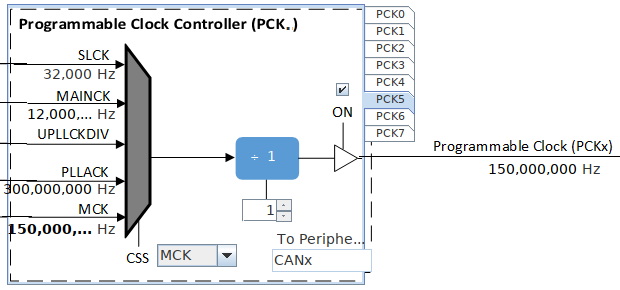
\includegraphics[width=\textwidth]{./Figures/Clock.png}
    \caption{Diagrama de configuración de las señales de reloj.}
	\label{fig:clock}
\end{figure}

El siguiente paso en la etapa de diseño fue la selección de las instancias de los periféricos del integrado.
Es posible que dos periféricos compartan parte del circuito interno o terminales del encapsulado.
Esta situación puede generar una disminución en las funcionalidades o una total incompatibilidad.
Finalmente, se seleccionaron instancias completamente disjuntas.

Luego de seleccionar las instancias de los periféricos, se configuraron para realizar un \emph{loopback}.
La configuración se realizó de la siguiente manera:

\begin{itemize}
    \item \emph{CAN}: se utilizó el \emph{MCAN1} con una configuración de \emph{loopback} interna, como se puede ver en la figura \ref{fig:canloopback}.
    \item \emph{PIO}: se configuraron dos terminales del dispositivo bajo prueba.
        El primero como salida sin \emph{latch} y el segundo como entrada sin circuito anti rebote.
    \item \emph{SPI}: la configuración elegida fue por defecto ya que el \emph{loopback} se logró conectando \emph{TX} y \emph{RX} con un cable.
    \item \emph{UART}: se configuró el periférico con una velocidad de 9600 baudios, 8 bits de datos y sin bits de paridad.
    \item \emph{Watchdog}: el disparo se configuró con un contador en 4095 cuentas.
        Este valor se estimó entre dos y cinco ejecuciones del \emph{loop} principal.
\end{itemize}

\begin{figure}[htbp]
	\centering
	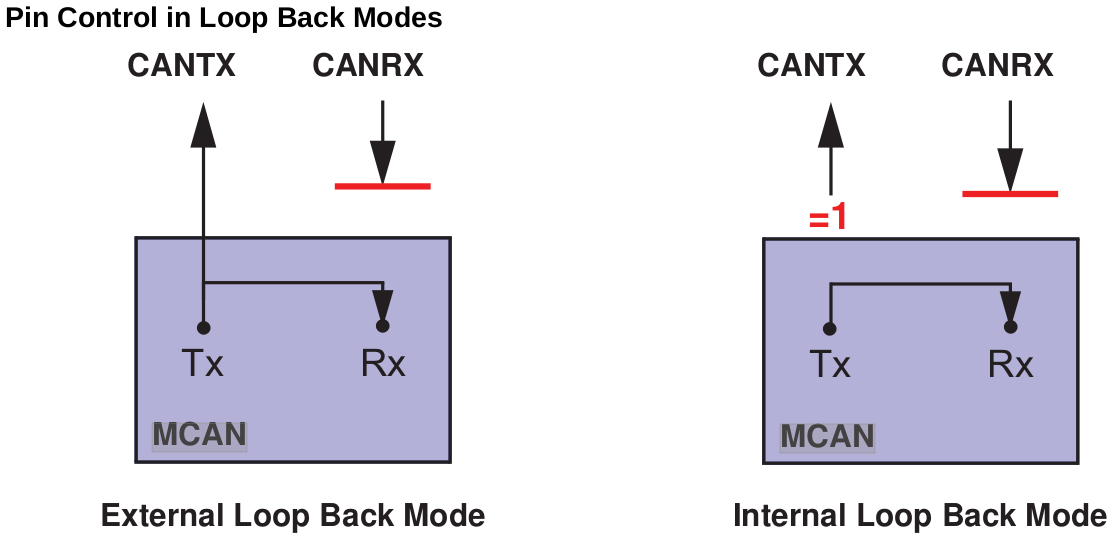
\includegraphics[width=0.8\textwidth]{./Figures/canloopback.png}
    \caption{Diagrama de \emph{loopback} del periférico \emph{CAN}\protect\footnotemark.}
	\label{fig:canloopback}
\end{figure}

\footnotetext{Imagen tomada de la hoja de datos del dispositivo bajo prueba \citep{ARTICLE:dutdatasheet}.}

Como se puede ver en la figura \ref{fig:labo}, se priorizaron los \emph{loopbacks} físicos externos.
Cuando esta estrategia no fue posible, se optó por internos provistos por el fabricante.
Finalmente, en los casos que las dos primeras opciones fueron imposibles, se utilizó una estrategia de \emph{software}.
En la tabla \ref{tab:perifericos} se puede ver un resumen de las estrategias aplicadas.

\begin{table}[h]
	\centering
	\caption[Estrategias de depuración]{Comparación entre estrategias de depuración}

	\begin{tabular}{l c c}    
		\toprule
        \textbf{Periférico} & \textbf{Validación}       & \textbf{Detección en un ciclo}\\
		\midrule
		CAN                 & Loopback interno          & Sí\\		
		PIO                 & Loopback externo          & No\\
		SPI                 & Loopback externo          & Sí\\
		UART                & Lógica en firmware        & No\\
		Watchdog            & Lógica en inyector        & No\\
		\bottomrule
		\hline
	\end{tabular}
	\label{tab:perifericos}
\end{table}

\begin{figure}[htbp]
	\centering
	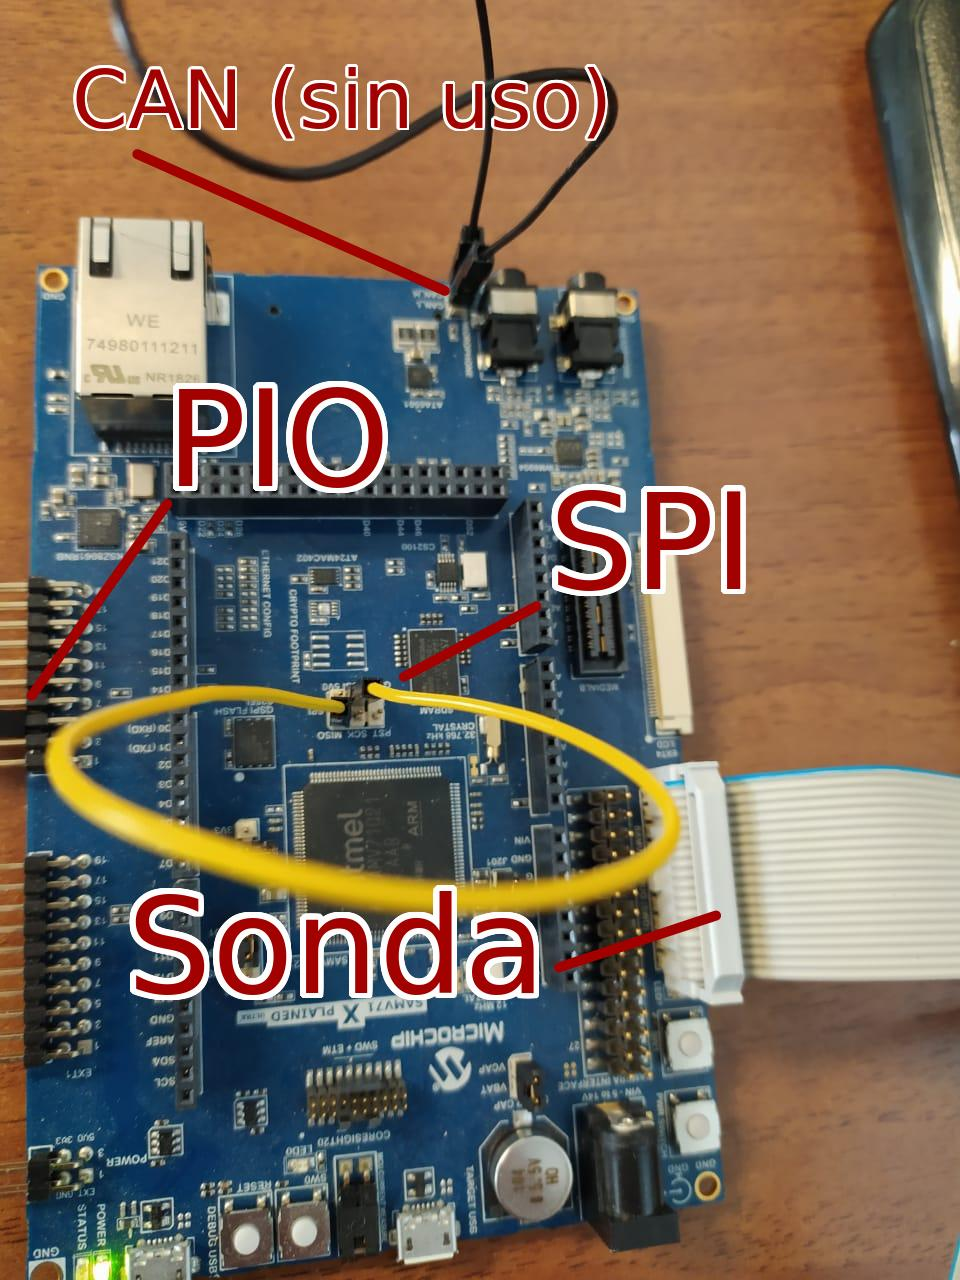
\includegraphics[width=\textwidth]{./Figures/labo.jpeg}
    \caption{Fotografía del dispositivo bajo prueba.}
	\label{fig:labo}
\end{figure}

\newpage

Una vez configurados los componentes de \emph{hardware} del dispositivo bajo prueba; se procedió a diseñar el \emph{firmware}.
Se comenzó con la estructura que define los reportes de estado del dispositivo bajo prueba.
Los reportes están formados por 2 bytes, el primero es el carácter ``F'' y marca el inicio del reporte mientras que el segundo byte lleva la información del estado de los periféricos.
En el código \ref{cod:structs} se puede ver la implementación del segundo byte del reporte.

\begin{lstlisting}[language=C,label=cod:structs,caption=Definición de la estructura de reportes.]  % Start your code-block

#define BIT 1

struct status_bitfield_t
{
    uint8_t CAN:BIT;
    uint8_t SPI:BIT;
    uint8_t PIO:BIT;
    uint8_t WATCHDOG:BIT;
}__attribute__((packed));

typedef union
{
    struct status_bitfield_t status_of;
    uint8_t packed;
}report_t;

\end{lstlisting}

En el código \ref{cod:loop} se puede observar la implementación del lazo principal.
Es importante notar que en la línea 10 se utilizó la \emph{union} para transformar el reporte en caracteres legibles para una persona.
En la figura \ref{fig:firmwareflow} se puede observar el flujo completo del programa.

\begin{lstlisting}[language=C,label=cod:loop,caption=Lazo principal del \emph{firmware} de autoevaluación.]  % Start your code-block

while ( true )
{
    SYS_Tasks ( );
    report.status_of.CAN = validate_CAN();
    report.status_of.PIO = validate_PIO();
    report.status_of.SPI = validate_SPI();
    report.status_of.WATCHDOG = NORMAL;
    
    buffer[FRAME_START] = 'F';
    buffer[FLAGS_INDEX] = report.packed + 'A';
    USART1_Write(&buffer[0], FRAME_SIZE);
    
    WDT_Clear();
}

\end{lstlisting}

\begin{figure}[htbp]
	\centering
	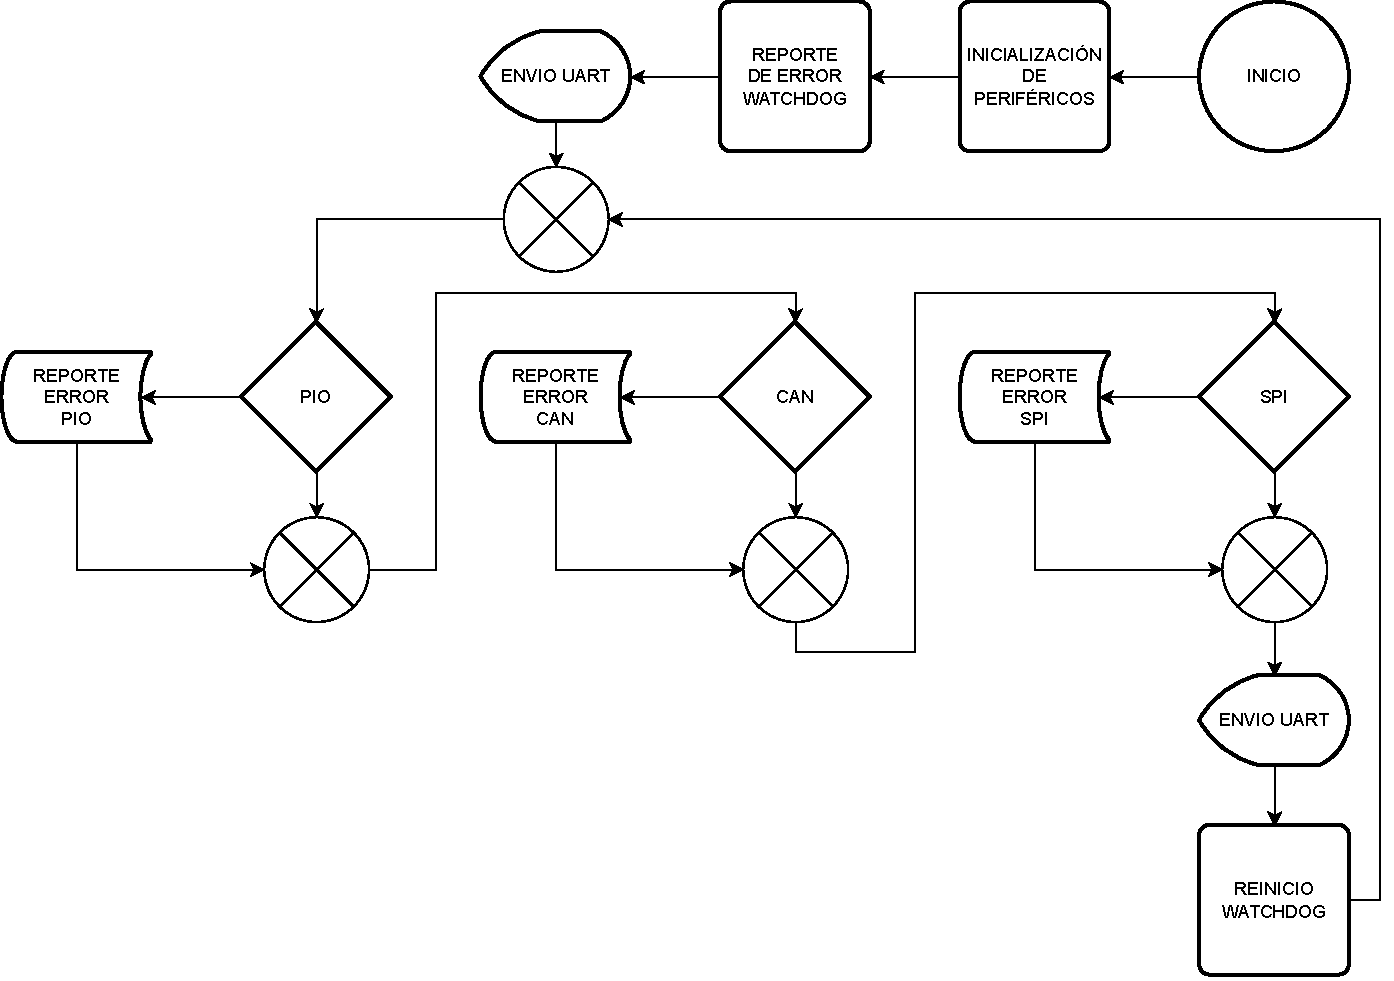
\includegraphics[width=\textwidth]{./Figures/firmwareflow.pdf}
    \caption{Flujo del \emph{firmware} de autoevaluación.}
	\label{fig:firmwareflow}
\end{figure}

\newpage

\section{Interfaz de programación de aplicaciones}
\label{sec:api}

% técnica RAII
% conexión como recurso
La interfaz de programación de aplicaciones tiene la función de abstraer al inyector de errores del servidor \emph{OCD}.
Esto se logró con los siguientes paradigmas y patrones de diseño:

\begin{itemize}
    \item Programación orientada a objetos \emph{(OOP)}: este paradigma de diseño se basa en agrupar en una unidad lógica las funcionalidades y estados que tengan un alto grado de acoplamiento.
        Esto significa que la funciones que tienen efectos colaterales junto a los datos mutados se encapsulan dentro de una construcción denominada objeto.
        Entonces, el principal objetivo de un objeto es contener dentro suyo los efectos colaterales.
        Además, el lenguaje de programación \emph{Python 3} permite, a través de una \emph{class}, modelar un tipo de dato para instanciar a un objeto.
        Finalmente, este patrón se utilizó para contener las funciones de lectura y escritura de registros y memorias.
    \item \emph{Resource Acquisition Is Initialization (RAII)}: este patrón de diseño consiste en modelar el ciclo de vida de un recurso con la implementación de un objeto.
        Un recurso es todo aquello que requiera mantenimiento luego de su uso, como por ejemplo: liberar memoria, cerrar una conexión o unir dos hilos de un programa.
        Esto se logra al adquirir un recurso cuando se invoca el constructor de una \emph{class}, por ejemplo, la conexión con la sonda de depuración se realiza durante la instanciación de un objeto llamado conexión.
        Luego, cuando se desea cerrar la conexión se invoca al destructor del objeto.
        Dentro de esta función se encuentra el código para cerrar de forma ordenada la conexión con la sonda y el dispositivo bajo prueba.
        Finalmente, este patrón de diseño hace que el programa maneje de forma robusta los recursos ya que está garantizada la ejecución de los destructores.
\end{itemize}

En el código \ref{cod:halted} se puede observar un ejemplo de \emph{RAII} donde se maneja como recurso la detención del núcleo del dispositivo bajo prueba.
Esto permite que frente a una excepción del proceso que esté utilizando la interfaz de programación de aplicaciones, el núcleo pueda continuar operando.
Finalmente, se posibilita recuperar el proceso sin tener que reiniciar el dispositivo bajo prueba.

\begin{lstlisting}[language=Python,label=cod:halted,caption=Ejemplo de \emph{Resource Acquisition Is Initialization (RAII)}.]  % Start your code-block

class Halted():
    def __init__(self, target):
        self.target = target

    def __enter__(self):
        self.target.halt()

    def __exit__(self, exc_type, exc_val, traceback):
        self.target.resume()

\end{lstlisting}

Los patrones de diseño utilizados permiten escribir funciones expresivas y robustas.
Como se puede ver en el código \ref{cod:haltedexample}, es fácil comprender lo que sucede.
En la línea 2 se detiene el núcleo y en la línea 3 se lee una posición de memoria.
Luego, en la línea 4 el núcleo reanuda su funcionamiento y finalmente, se retorna el valor leído.

\newpage

\begin{lstlisting}[language=Python,label=cod:haltedexample,caption=Ejemplo de uso de \emph{RAII}.]  % Start your code-block

def readMemory(self, addr: int):
    with Halted(self.target):
        val = self.target.read_memory(addr)
    return val

\end{lstlisting}

En la tabla \ref{tab:funcionalidades} se puede observar un resumen de las funcionalidades y sus estrategias de abstracción.

\begin{table}[h]
	\centering
	\caption[Funcionalidades abstraidas]{Funcionalidades abstraídas}

	\begin{tabular}{l c c}    
		\toprule
        \textbf{Funcionalidad}     & \textbf{Patrón de diseño} & \textbf{Acceso}\\
		\midrule
		Conexión al integrado      & RAII                      & Público\\		
		Detener el núcleo          & RAII                      & Privado\\
		Registros CORE: read/write & OOP                       & Público\\
		Memoria SDRAM: read/write  & OOP                       & Público\\
		\bottomrule
		\hline
	\end{tabular}
	\label{tab:funcionalidades}
\end{table}

Finalmente, se logró abstraer el ciclo de vida de la sesión de depuración que se muestra en la figura \ref{fig:debugsession}.

\begin{figure}[htbp]
	\centering
	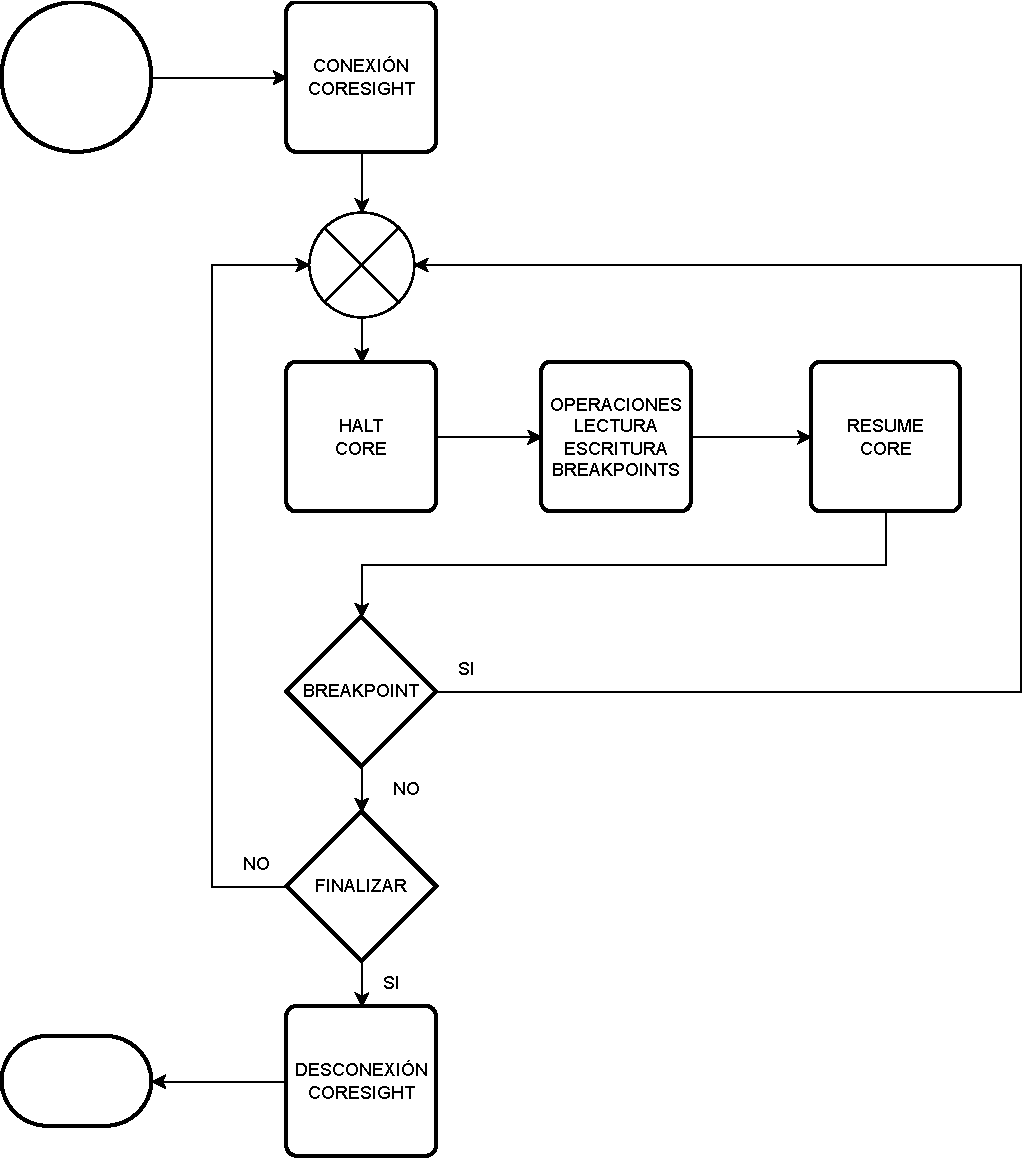
\includegraphics[width=0.9\textwidth]{./Figures/debugsession.pdf}
    \caption{Flujo de una sesión de depuración.}
	\label{fig:debugsession}
\end{figure}

\section{Sistema de inyección de \emph{soft-errors}}
\label{sec:sise}

Una vez lograda la interfaz de programación de aplicaciones explicada en la sección \ref{sec:api}, se pudo construir el inyector por consola de comandos que se muestra en la figura \ref{fig:siseblocks}.
Para lograr que el usuario utilice el programa se creó un sistema de archivo de configuración y un cliente de terminal en texto plano.
El archivo de configuración se genera en formato \emph{YAML} y se encarga de:

\begin{itemize}
    \item Definir si el controlador de ensayos debe recoger los reportes del dispositivo bajo prueba.
    \item Configurar el puerto serie del ordenador.
    \item Definir la simulación:
        \begin{itemize}
            \item El tipo de distribución para usar en el planificador de ensayos.
            \item La tasa de inyección de errores.
            \item La duración del tiempo de exposición en un registro o posición de memoria.
            \item La secuencia de exposición de los registros.
        \end{itemize}
\end{itemize}

% Configuración

En el código \ref{cod:yaml} se puede observar un archivo de configuración.
En particular, la configuración que el sistema ofrece como ejemplo al usuario.
Es importante notar que no se hace referencia a la sesión de depuración.
Finalmente, el ensayo se expresa en términos de parámetros de radiación.

Para facilitar la tarea del usuario, una vez instalado el sistema no es necesario trabajar en una carpeta en particular.
El inyector se puede invocar desde cualquier sitio donde el intérprete de Python 3 tenga permisos de ejecución.
El operador puede entonces crear una carpeta del ensayo.
Luego, crear un archivo de configuración y lanzar desde allí mismo la secuencia de inyecciones.
Finalmente, el sistema genera el reporte correspondiente en esa ruta.

\begin{lstlisting}[language=Python,label=cod:yaml,caption=Ejemplo de configuración de ensayo.]  % Start your code-block

# Perfil determina el tipo de ensayo a realizar
# 'simulador' solo genera inyecciones mientras
# que 'evaluador' recoge y procesa los
# reportes del DUT.
Perfil: 'simulador'

# Interfaz define el puerto serie donde se
# conecto el DUT.
Interfaz:
  puerto: '/dev/ttyACM0'
  baudios: 9600

# Simulacion define la forma de inyectar errores
Simulacion:
  distribucion: 'Poisson'
  tasa: 0.5
  duracion: 5
  registros: 'secuencial'

\end{lstlisting}

% Consola

La interfaz por consola se logró al utilizar el \emph{standar input} y el \emph{standar output} del proceso padre.
En el caso de una sesión iniciada por un humano, el emulador de terminal del sistema.
En una primera iteración de la consola se realizó una interfaz ASCII con la biblioteca \emph{curses}.
Sin embargo, el cliente prefirió una interfaz por texto plano para facilitar el \emph{parsing} de un sistema de integración continua.
En particular, el módulo de \emph{CI/CD} de \emph{Gitlab}.

El usuario invoca el programa al ejecutar el comando \texttt{sise}.
Luego la consola responde con la leyenda \texttt{Ingrese el archivo de configuración > }.
Se escribe la ruta y nombre del archivo a utilizar y el sistema lanza el ensayo.
El reporte generado se persiste en la carpeta donde se inició el programa.

% Planificador de ensayos

Con la información suministrada por el archivo de configuración y la consola, se puede iniciar el planificador de ensayos.
Este módulo tiene la función de generar una variable aleatoria que genera tiempos entre inyecciones de errores.
La variable aleatoria se construye con los datos de distribución y tasa de error.
El proceso aleatorio se repite hasta que la sumatoria de los tiempos generados sea igual o mayor al tiempo deseado del ensayo.
Luego, se asigna cada tiempo a un registro del núcleo en particular.
Esta asignación se realiza según la configuración del usuario.
Finalmente, se entrega la planificación al controlador de ensayos.

% Controlador de ensayos

El controlador de ensayos es un hilo del programa que tiene la misión de ejecutar una planificación de ensayos.
Su ejecución se basa en la interfaz de abstracción de aplicaciones explicada en la sección \ref{sec:api}.
Luego, tiene la responsabilidad de observar el tiempo de ejecución del dispositivo bajo prueba.
Cuando el momento es adecuado, el controlador invoca una función de \emph{bit flip}.
El bit a invertir se determina en el momento de inyección con una variable aleatoria uniforme.
Finalmente, cuando el controlador consume la totalidad de la planificación, envía una señal para solicitar el \emph{join} con el hilo principal del programa.

% Generador de reportes

El generador de reportes es un hilo que escucha el puerto serie del ordenador.
Mientras dura el ensayo, almacena todos los mensajes entrantes y los acumula junto a un \emph{timestamp}.
De la misma manera, persiste las inyecciones realizadas como tuplas.
Estas tuplas tienen todos los datos relevantes de la inyección junto a un \emph{timestamp}.
Cuando el ensayo finaliza, recibe una señal desde el hilo principal del programa que le ordena hacer un \emph{join}.
Luego, el generador de reportes deja de escuchar el puerto serie y al controlador de ensayos.
Seguidamente, se procede a construir un reporte en formato de tabla de \emph{MS Excel} y \emph{CSV}.
Para lograrlo, se genera una relación de causalidad entre errores inyectados y respuestas del dispositivo bajo prueba.
Finalmente, se generan los archivos en la carpeta donde el comando \texttt{sise} fue lanzado.

% Funcionamiento concurrente

La mayor dificultad del inyector fue el manejo concurrente de los hilos del controlador de ensayo y el generador de reportes.
En particular, porque ambos hilos comparten el uso del puerto serie.
Esta situación genera una condición de carrera que se tuvo que manejar.
Luego, se decidió evitar candados y semáforos al explotar la topología de \emph{bus} en árbol del protocolo \emph{USB}.
De esta manera, la conexión con la UART y el DAP se trató como si estuviesen conectados en puertos físicos diferentes.
Esta decisión de diseño tiene la ventaja de no incrementar el error de las mediciones de tiempo.
Un error en la medición generaría relaciones de causalidad incorrectas y por lo tanto los informes no serían confiables.
Sin embargo, se introdujo un punto de falla al depender de la capacidad de la sonda de depuración y su gestión de su árbol de dispositivos.
Finalmente, en la figura \ref{fig:concurrencia} se puede observar un diagrama con los hilos del programa.

\begin{figure}[htbp]
	\centering
	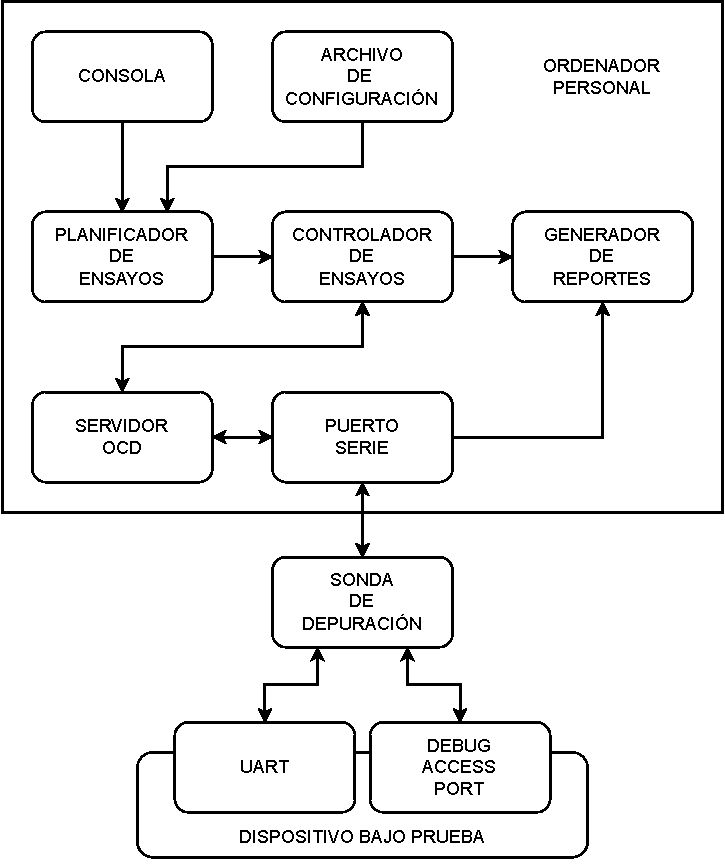
\includegraphics[width=\textwidth]{./Figures/siseblocks.pdf}
    \caption{Diagrama en bloques del sistema de inyección de soft-errors.}
	\label{fig:siseblocks}
\end{figure}

\begin{figure}[htbp]
	\centering
	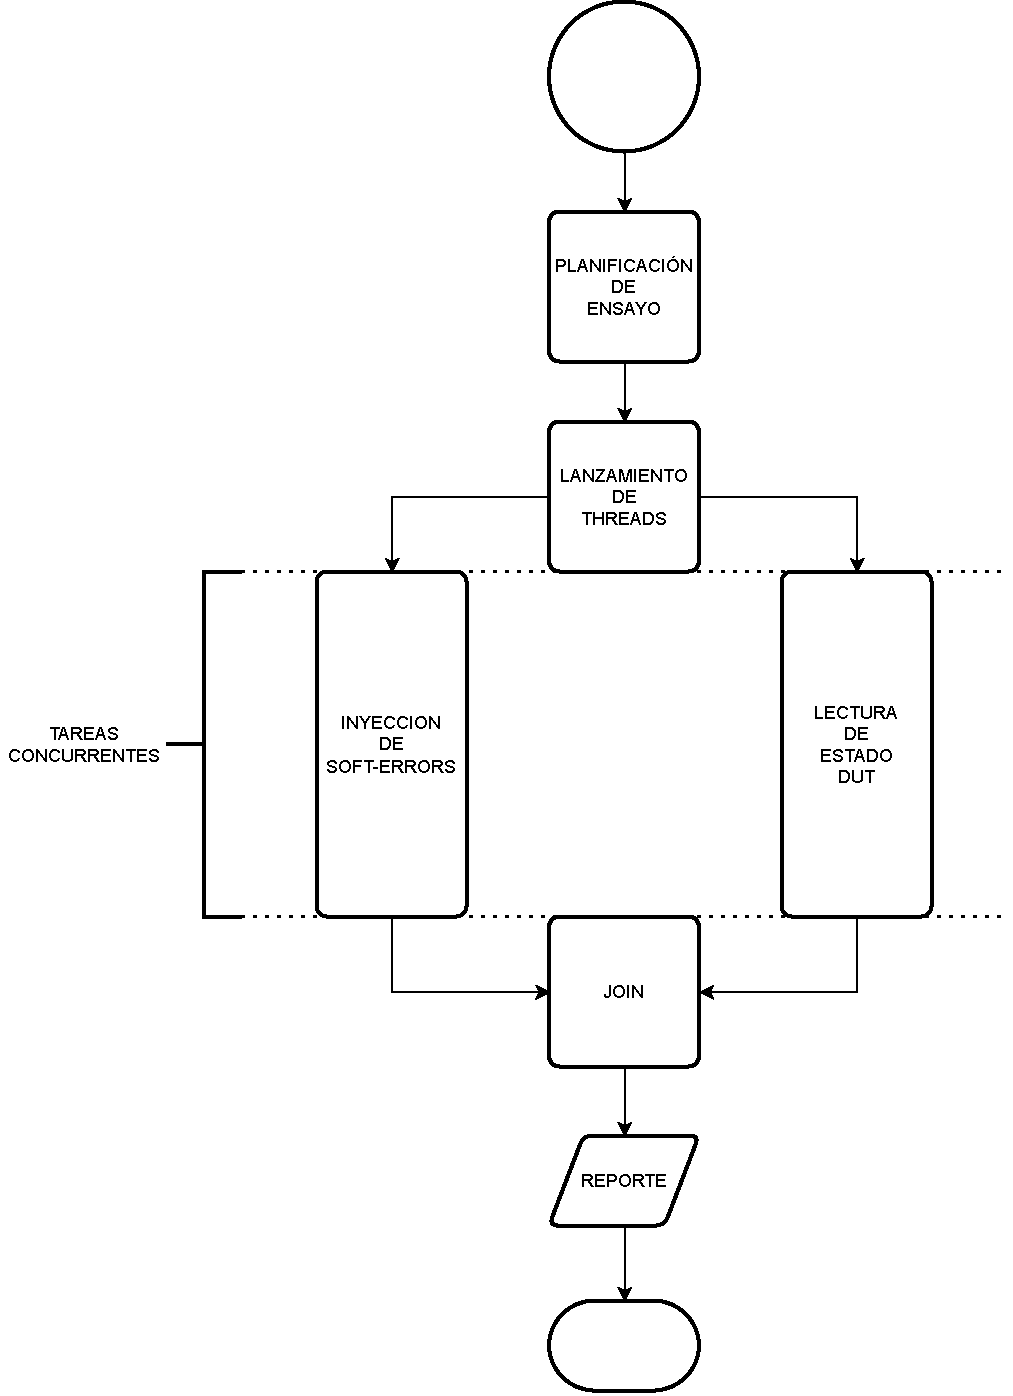
\includegraphics[width=\textwidth]{./Figures/concurrencia.pdf}
    \caption{Flujo de tareas concurrentes.}
	\label{fig:concurrencia}
\end{figure}

\section{Biblioteca para el desarrollo de ensayos}
\label{fig:biblioteca}

Para que el usuario pueda realizar sus propios ensayos, se creó una biblioteca que le provee la funcionalidad necesaria.
Esta biblioteca se divide en dos partes:

\begin{itemize}
    \item Funcionalidades del núcleo.
    \item Funcionalidades de la memoria.
\end{itemize}

Para facilitar la interacción con el núcleo se implementó una lista con los nombres de los registros.
De esta manera, se facilita el uso de las funciones.
En el código \ref{cod:corereg} se puede observar la colección que se le ofrece al diseñador.

\begin{lstlisting}[language=Python,label=cod:corereg,caption=Lista de registros accesibles por el usuario.]  % Start your code-block

CORE_REGISTERS = [
    'lr', 'pc', 'sp', 'xpsr', 'r0', 'r1', 'r2', 'r3',
    'r4', 'r5', 'r6', 'r7', 'r8', 'r9', 'r10', 'r11', 'r12'
]

\end{lstlisting}

Las funcionalidades ofrecidas para manipular el núcleo del integrado se muestran en el código \ref{cod:coreapi}.
Los detalles son los siguientes:

\begin{itemize}
    \item En la línea 6 se muestra el uso de la función de lectura de registros.
        Se invoca a partir del objeto de conexión y su argumento es el nombre del registro a leer.
    \item En la línea 10 se puede observar el uso del método de escritura de registros.
        Necesita como argumento el nombre del registro y el valor a escribir.
        Luego, la función retorna una tupla con los valores previos y posteriores a la escritura.
    \item En la línea 15 se ve una llamada a la función de \emph{bit flip} del registro del núcleo.
        Se debe indicar el nombre del registro y la posición del bit a invertir.
        Finalmente, se retorna el valor previo y posterior al llamado del método.
\end{itemize}

\newpage

\begin{lstlisting}[language=Python,label=cod:coreapi,caption=Ejemplo de uso en registros del núcleo.]  % Start your code-block

import sise.library as sise

dut = sise.Connection()

# Lectura del registro del CORE
rreg = dut.readRegister('pc')
print("PC:", rreg)

# Escritura del registro del CORE
wreg = writeRegister('r0', 0xffffffff)
print("(old, new):", wreg)

# Bit-flip en registro del CORE
bit = 2
bfreg = bitFlipRegister('r1', bit)
print("(old, new):", bfreg)

del(dut)

\end{lstlisting}

Para interactuar con la memoria se dispone de las funciones demostradas en el código \ref{cod:menapi}.
Los métodos se detallan a continuación:
\begin{itemize}
    \item Línea 7: el método permite realizar una lectura del dato en una posición de memoria.
        El argumento es una dirección alineada de la memoria y el retorno es el valor de una palabra de 32 bits.
    \item Línea 12: esta función se utiliza para escribir una posición alineada de memoria.
        Se necesita pasarle una dirección y un valor a escribir.
        Finalmente, retorna una tupla con el dato previo y posterior a la ejecución del método.
    \item Línea 18: la subrutina posibilita hacer un \emph{bit flip} en una posición de memoria.
        El método toma como argumento una posición alineada de memoria y el bit a invertir.
        Luego de su ejecución, se retorna el valor previo y posterior a la inversión.
\end{itemize}

\begin{lstlisting}[language=Python,label=cod:menapi,caption=Ejemplo de uso en memoria.]  % Start your code-block

import sise.library as sise

dut = sise.Connection()

# Lectura de memoria
addr = 0x20400004
rmen = readMemory(addr)
print("men:", rmen)

# Escritura de memoria
addr = 0x20400008
wmen = writeMemory(addr, 0xfafafafa):
print("(old, new):", wmen)

# Bit-flip en memoria
addr = 0x20400000
bit = 0
bfmen = dut.bitFlipMemory(addr, bit)
print("(old, new):", bfmen)

del(dut)

\end{lstlisting}

% Chapter Template

\chapter{Ensayos y resultados} % Main chapter title

\label{Chapter4} % Change X to a consecutive number; for referencing this chapter elsewhere, use \ref{ChapterX}

En este capítulo se describe la estrategia de pruebas adoptada para determinar que el sistema se comporta de forma esperada.

%----------------------------------------------------------------------------------------
%	SECTION 1
%----------------------------------------------------------------------------------------

\section{Laboratorio remoto}
\label{sec:lab}

Durante las primeras etapas del desarrollo no se disponía en Buenos Aires del dispositivo bajo prueba.
Por esta razón, se montó un laboratorio remoto en San Carlos de Bariloche.
Se dispuso una placa de evaluación \emph{SAM V71 Xplained Ultra} conectada a un ordenador dentro de la red de INVAP S.E.
La conexión entre la placa y el ordenador se logró a través de una sonda de depuración \emph{Segger J-32}.

Para poder acceder al laboratorio remoto que se muestra en la figura \ref{fig:remotelab} se necesitó:

\begin{itemize}
    \item Credenciales de acceso y conexión a la VPN de INVAP S.E.
    \item Crear un túnel SSH con el ordenador remoto.
\end{itemize}

El túnel SSH se generó con \emph{X11 forwarding} habilitado.
De esta manera, se pudo generar ventanas gráficas en el ambiente local.
Además, las operaciones de consola se integraron al ordenador personal con una sesión de Tmux.
Finalmente, se logró implementar una interfaz de control del laboratorio remoto con una apariencia idéntica al ambiente local.

\begin{figure}[htbp]
	\centering
	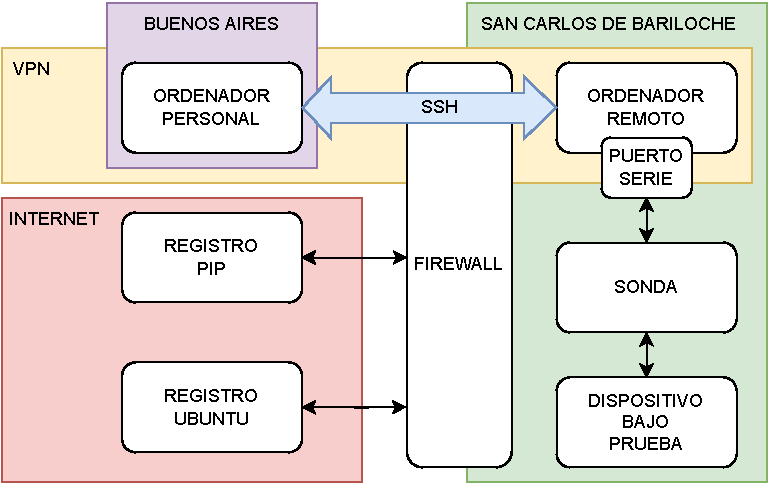
\includegraphics[width=\textwidth]{./Figures/vpn.pdf}
    \caption{Diagrama en bloques del laboratorio remoto.}
	\label{fig:remotelab}
\end{figure}

Para poder instalar las dependencias y los servidores OCD evaluados, se habilitaron los puertos necesarios que permitieron al ordenador remoto conectarse a los recursos en la Internet.
Sin embargo, algunos recursos debieron ser compilados en el \emph{host} y la transferencia de los \emph{tarballs} se realizó por medio de \emph{Secure Copy Files (scp)}.

Con el laboratorio remoto montado, se procedió a realizar las siguientes pruebas:
\begin{itemize}
    \item Pruebas de configuración de sondas de depuración y compatibilidad con servidores OCD.
    \item Pruebas de acceso al dispositivo bajo prueba.
\end{itemize}

Las pruebas referidas a la sonda de depuración arrojaron como resultado lo siguiente:

\begin{itemize}
    \item El modo de \emph{boot} de la sonda determina el nivel de acceso al dispositivo bajo prueba.
    \item Para lograr inyecciones de \emph{soft-errors} la sonda de depuración debe poder iniciar en modo \emph{CMSIS-DAP}.
    \item Si la sonda de depuración no se encuentra en modo \emph{CMSIS-DAP}, \emph{PyOCD} solo puede realizar escritura en la memoria \emph{flash}.
    \item Cambiar de modo una sonda de depuración requiere reiniciarla.
        Por lo tanto, no es factible realizar cambios de configuración luego de iniciado un ensayo.
\end{itemize}

Las pruebas referidas al acceso al dispositivo bajo prueba tuvieron los siguientes resultados:

\begin{itemize}
    \item Si no se dispone de un \emph{Device Family Pack (DFP)}, \emph{PyOCD} se conecta al dispositivo bajo prueba y lo identifica como \emph{Generic Cortex-M}.
    \item Bajo la identificación de \emph{Generic Cortex-M} se puede acceder a todos los registros de núcleo.
    \item Bajo la identificación de \emph{Generic Cortex-M} se puede acceder a la memoria \emph{SDRAM} y reconoce como error una posición desalineada.
    \item Bajo la identificación de \emph{Generic Cortex-M} se puede acceder a otras direcciones del integrado solo en modo lectura.
        Si se intenta ingresar en modo escritura no sucede ningún cambio pero el servidor OCD no responde con un error.
        Su respuesta es de operación exitosa, pero no se manifiestan cambios.
\end{itemize}

PyOCD posee un módulo de búsqueda y descarga de DFP, sin embargo, su funcionamiento no es confiable y genera una excepción durante su ejecución.
Se intentó verificar su funcionamiento en otras plataformas y se pudo observar que su desarrollo fue realizado en el lenguaje de programación \emph{Rust}.
Este módulo hizo imposible instalar el servidor OCD en una \emph{single board computer}.
Dado que, su compilador consume una cantidad de memoria que supera el \emph{hardware} disponible en placas como \emph{Raspberry Pi 4B}.
Se pudo verificar que este es el único módulo escrito en \emph{Rust}, pero no es posible desacoplarlo del servidor OCD.
Finalmente, PyOCD tiene una limitación de plataformas compatibles que podría ser sorteada con \emph{cross} compilación.

La única dificultad en el uso del laboratorio remoto se presentó en las pruebas de la sonda de depuración.
Muchas de las pruebas requirieron reiniciar la sonda y esto solo es posible al desconectar el cable \emph{USB}.
La operación debió ser realizada por el co-director de este trabajo.
En la tabla \ref{tab:funcionalidades}, se puede ver un resumen de las funcionalidades del laboratorio remoto.
Las funcionalidades con tres marcas tienen el mismo nivel de servicio que el laboratorio local, las de dos marcas tienen un nivel algo inferior y las que tienen solo una marca tienen un nivel de servicio bajo.

\begin{table}[h]
	\centering
	\caption[Resumen del laboratorio remoto]{Resumen del laboratorio remoto.}

	\begin{tabular}{l c}    
		\toprule
        \textbf{Funcionalidad}             & \textbf{Nivel de servicio} \\
		\midrule
		Carga de binarios en DUT           & ++  \\		
		Comunicación con registro PIP      & +++ \\
		Comunicación con registro Ubuntu   & +++ \\
		Comunicación con debug access port & +++ \\
		Comunicación con UART              & +   \\
		\bottomrule
		\hline
	\end{tabular}
	\label{tab:funcionalidades}
\end{table}

\section{Ensayos de inyector}
\label{sec:testinyector}

El inyector de \emph{soft-errors} se sometió a ensayos en los siguientes ambientes:

\begin{itemize}
    \item Laboratorio remoto.
    \item Laboratorio local.
    \item Dispositivo alternativo \emph{NUCLEO-F429ZI}.
        Este último ambiente se puede ver en la figura \ref{fig:alternativo} y se utilizó para probar si el inyector es genérico.
        En particular, porque utiliza una sonda de depuración distinta.
\end{itemize}

\begin{figure}[htbp]
	\centering
	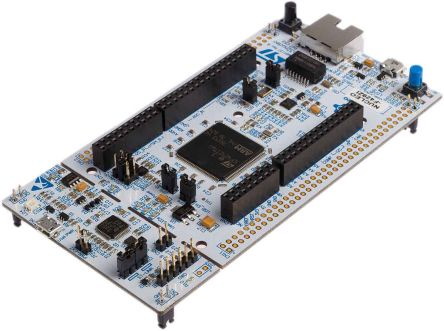
\includegraphics[width=0.8\textwidth]{./Figures/alternativo.jpg}
    \caption{Dispositivo alternativo \emph{NUCLEO-F429ZI}.}
	\label{fig:alternativo}
\end{figure}

Se generaron múltiples archivos de configuración para definir distintos casos de prueba.
Luego, se corrieron los ensayos en los tres ambientes y se compararon los resultados.
Además, se usó una variante adicional en el dispositivo alternativo.
Se probó el comportamiento del inyector sobre un blanco con \emph{mbedOS}.
Finalmente, en la tabla \ref{tab:resensayos} se puede observar un resumen de los resultados obtenidos.
En la tabla se marca con tres cruces los ensayos que arrojaron resultados sobresalientes, con dos cruces los ensayos que mostraron inconvenientes mínimos y con una cruz los ensayos con resultados insatisfactorios.

\begin{table}[h]
	\centering
	\caption[Resumen de ensayos]{Resumen de ensayos}

	\begin{tabular}{l c c c}    
		\toprule
        \textbf{Ensayo}                 & \textbf{Lab. local} & \textbf{Lab. remoto} & \textbf{DUT alterno} \\
		\midrule
		Escritura SDRAM                 & +++                 & +++                  & +++ \\
		Escritura registros CORE        & +++                 & +++                  & +++ \\
		Funcionalidades extras          & ++                  & ++                   & +++ \\
		Halt CORE                       & +++                 & +++                  & +++ \\
		Lectura SDRAM                   & +++                 & +++                  & +++ \\
		Lectura registros CORE          & +++                 & +++                  & +++ \\		
		Uso concurrente de puerto serie & +++                 & +                    & +++ \\
        Resume CORE                     & +++                 & +++                  & +++ \\
		\bottomrule
		\hline
	\end{tabular}
	\label{tab:resensayos}
\end{table}

El dispositivo alternativo arrojó los mejores resultados porque PyOCD tiene el \emph{Device Family Pack}.
Por otro lado, el laboratorio remoto tuvo malos resultados en las pruebas de concurrencia.
Esto fue así ya que se debía pedir ayuda al personal de INVAP S.E. cada vez que la sonda necesitaba ser reiniciada. 

\section{Validación con el cliente}
\label{sec:validacion}

La etapa final del proceso de pruebas fue una serie de demostraciones realizadas al cliente.
Luego de cada demostración se indicaban las correcciones a realizar.
Seguidamente, se mejoraba el código y se repetía la demostración.
Estos ciclos de iteraciones tenían una frecuencia de 15 días.
Finalmente, se llegó al cumplimiento total de los requerimientos como se puede ver en la tabla \ref{tab:validacion}

\begin{table}[h]
	\centering
	\caption[Resumen de la validación con el cliente]{Resumen de la validación con el cliente}

	\begin{tabular}{l c}    
		\toprule
        \textbf{Expectativas}     & \textbf{Cumplimiento} \\
		\midrule
		Acceso a memoria          & +++                   \\
		Acceso al CORE            & +++                   \\
		Biblioteca de ensayos     & +++                   \\		
		Capacidad de bit-flip     & +++                   \\
		Configuración del sistema & +++                   \\
		Distribución de errores   & +++                   \\
		Validación de periféricos & +++                   \\
        Generación de reportes    & +++                   \\
		\bottomrule
		\hline
	\end{tabular}
	\label{tab:validacion}
\end{table}

En la figura \ref{fig:demobitflip} se puede observar una demostración del acceso a memoria SDRAM.
Se puede ver que la terminal está dividida en las siguientes partes:

\begin{itemize}
    \item Sección izquierda: se hizo una demostración paso a paso.
        Primero, se importó la biblioteca dentro del espacio de trabajo.
        Luego, se conectó al dispositivo y se cargó una dirección de memoria y el bit a invertir.
        Seguidamente, se realizó una inversión y se mostró el valor previo y posterior al \emph{bit flip}.
        Finalmente, se cerró la conexión con el dispositivo alternativo.
    \item Sección derecha: se observa el mapa de memoria SDRAM del dispositivo alternativo.
        Se usó para mostrarle al cliente las direcciones de memoria ensayadas.
\end{itemize}

Este ensayo además de demostrar el acceso a memoria SDRAM también ejercita la capacidad de realizar \emph{bit flip}.
Finalmente, el cliente consideró que se habían cumplido todos los requisitos y que el trabajo se encontraba finalizado.

Los ensayos finales se volvieron a reproducir en presencia de un estudiante de la especialización en sistemas embebidos quién actualmente utiliza la herramienta en el marco de su proyecto final.

\begin{figure}[htbp]
	\centering
	\includegraphics[width=\textwidth]{./Figures/demo_bitflip.png}
    \caption{Demostración de acceso a memoria.}
	\label{fig:demobitflip}
\end{figure}
 
\chapter{Conclusiones}
\label{Chapter5}

Este capítulo explica de forma breve el cierre del trabajo realizado, sus logros y futuro.

\section{Resultados obtenidos}
\label{sec:5resultados}

El trabajo logró cumplir las expectativas y requerimientos del cliente.
En particular, los siguientes objetivos:

\begin{itemize}
    \item Creación de un sistema de inyección de \emph{soft-errors} que permita evaluar técnicas de mitigación de errores.
    \item Acceso a la memoria volátil del dispositivo bajo prueba.
    \item Biblioteca para el diseño de ensayos en lenguaje \emph{Python 3}.
\end{itemize}

La recepción de este trabajo fue muy positiva; ya que en la actualidad, INVAP S.E. se encuentra en proceso de integrar la herramienta en su ambiente de desarrollo de satélites.
Además, el sistema realizado se utiliza dentro del marco de un proyecto final en la Especialización en Sistemas Embebidos.

\section{Trabajo futuro}
\label{sec:5futuro}

La investigación realizada durante la producción del trabajo sugiere que es posible agregar las siguientes funcionalidades:

\begin{itemize}
    \item Conexión entre el código fuente del dispositivo bajo prueba y el inyector de \emph{soft-errors}.
    \item Creación de instrucciones específicas para la inyección de \emph{single event functional interrupt}.
\end{itemize}
 

%----------------------------------------------------------------------------------------
%	CONTENIDO DE LA MEMORIA  - APÉNDICES
%----------------------------------------------------------------------------------------

\appendix % indicativo para indicarle a LaTeX los siguientes "capítulos" son apéndices

% Incluir los apéndices de la memoria como archivos separadas desde la carpeta Appendices
% Descomentar las líneas a medida que se escriben los apéndices

%% Appendix A

\chapter{Appendix Title Here} % Main appendix title

\label{AppendixA} % For referencing this appendix elsewhere, use \ref{AppendixA}

Write your Appendix content here.
%\include{Appendices/AppendixB}
%\include{Appendices/AppendixC}

%----------------------------------------------------------------------------------------
%	BIBLIOGRAPHY
%----------------------------------------------------------------------------------------

\Urlmuskip=0mu plus 1mu\relax
\raggedright
\printbibliography[heading=bibintoc]

%----------------------------------------------------------------------------------------

\end{document}  
